\lamina{img/fig02_p7.jpg}
\mainmatter
\capitulo{CAPÍTULO 0}{EL EXPERIMENTO EXPLICADO A MI MADRE}{O: Cómo leer este libro sin haber estudiado física}{}
\noindent \capital{M}{i} madre tiene ochenta años. Lee novelas, no artículos de \emph{Nature}. Cuando le expliqué este libro, me dijo: “Hijo, suena interesante, pero no entiendo nada de agujeros negros.”

Este capítulo es para ella. Y para ti, si tampoco entiendes nada de agujeros negros. No te preocupes: no necesitas entender física para entender este libro. Solo necesitas tres ideas, y las tres las conoces ya, aunque no sepas que se llaman de otra manera en física.

\seccion{\MakeLowercase{IDEA 1: LA BURBUJA}}
\noindent Has soplado burbujas de jabón. ¿Recuerdas el momento exacto en que una burbuja se cierra? El jabón se estira, se curva, y de repente tienes una esfera completa: un dentro y un fuera que antes no existían.

Eso es un horizonte.

No una línea en el mapa. Una frontera viva que separa lo interior de lo exterior. La burbuja no es el jabón —es la organización. Y lo que hace que la burbuja sea burbuja no es el aire dentro, sino la piel que lo encierra.

En física, cuando una estrella muere y colapsa sobre sí misma, crea algo parecido: una frontera donde el espacio se cierra sobre sí mismo. Esa frontera se llama “horizonte de sucesos”. Es el punto donde la luz deja de escapar. No porque haya una pared. Porque la geometría misma se dobla.

Pero aquí viene lo importante: este libro no dice que haya un agujero negro dentro de tu cabeza. Dice algo más curioso: que la conciencia —lo que te hace ser tú, el espacio donde ocurren tus pensamientos— podría tener la misma geometría que un horizonte. Una frontera que define un interior. Una burbuja que no es de jabón, sino de información.

\begin{fisica}
\lbl{En física esto se llama:} horizonte de sucesos.

\lbl{En la vida diaria es como:} la piel de una burbuja.
\end{fisica}
\seccion{\MakeLowercase{IDEA 2: EL OCÉANO Y LAS OLAS}}
\noindent El océano no está vacío cuando no hay olas. Está lleno de agua en estado de reposo. Las olas no son agua que viaja de lejos: son el agua local moviéndose de cierta manera. Cuando una ola rompe en la playa, el agua no ha llegado de ningún sitio: ha estado ahí todo el tiempo, cambiando de forma.

En física, el “vacío” no está vacío. Está lleno de un campo —un “océano” de posibilidad— del que emergen las partículas como las olas emergen del agua. Las partículas no son cosas que viajan por el vacío: son el vacío vibrando de cierta manera.

Este libro llama a ese océano el \textbf{reservorio}. Es el campo del que emergería la conciencia y al que retornaría. No es un lugar. Es una condición. Como el agua está para las olas, el reservorio está para los horizontes.

Las tradiciones orientales llevan siglos hablando de esto con otras palabras. El taoísmo lo llama \emph{Hun Dun}: el caos que es plenitud, antes de que exista la distinción. El \emph{Vedanta} lo llama \emph{Brahman}: la conciencia subyacente a toda forma. No son pruebas de la física. Son vocabularios distintos para intuir la misma estructura: que lo que parece separado —tú, yo, esta mesa— emerge de algo que no está separado en absoluto.

\begin{fisica}
\lbl{En física esto se llama:} vacío cuántico.

\lbl{En la vida diaria es como:} el océano antes de las olas.
\end{fisica}
\seccion{\MakeLowercase{IDEA 3: LA RED}}
\noindent Imagina una red de pesca tendida en el agua. La red no es los nudos individuales: es la forma que toman cuando están conectados. Si cortas un hilo, la red sigue siendo red, pero es una red distinta. Si cortas demasiados hilos, deja de ser red y se convierte en hilos sueltos.

La conciencia, según una teoría llamada IIT (Teoría de Información Integrada), es así: no está en ninguna neurona individual, sino en la forma en que las neuronas se conectan. La “red” de tu cerebro, cuando está suficientemente integrada, genera algo que no está en ninguna de sus partes: un punto de vista. Un “adentro”.

Eso es lo que la física llama \textbf{Phi (Φ)}: una medida de cuánto un sistema es más que la suma de sus partes. Un termostato tiene \emph{Phi} casi nulo. Un cerebro despierto tiene \emph{Phi} muy alto. Un cerebro bajo anestesia general muestra caída drástica de \emph{Phi}.

\begin{fisica}
\lbl{En física esto se llama:} Phi (Φ), información integrada.

\lbl{En la vida diaria es como:} qué tan “red” es una red.
\end{fisica}
\seccion{\MakeLowercase{CÓMO USAR ESTE LIBRO}}
\noindent No necesitas recordar los términos técnicos. Cuando veas una palabra que no entiendes, imagina la analogía:

\par\vspace{4pt}\begin{center}\small\renewcommand{\arraystretch}{1.15}\begin{tabularx}{\textwidth}{>{\raggedright\arraybackslash\hsize=0.98\hsize}X>{\raggedright\arraybackslash\hsize=1.02\hsize}X}\toprule
\thead{Término técnico} & \thead{Imagina…} \\ \midrule
Horizonte de sucesos & La piel de la burbuja \\[3pt]
Reservorio & El océano antes de las olas \\[3pt]
\emph{Phi} (Φ) & Qué tan “red” es una red \\[3pt]
\emph{Scrambling} & Echar tinta en agua: la información se mezcla pero no desaparece \\[3pt]
Entrelazamiento & Dos cuerdas de guitarra que, habiéndose afinado juntas, vibran al unísono \\[3pt]
Transición de fase & Agua que se convierte en hielo: misma molécula, forma distinta \\[3pt]
Soft hair / huella & La forma que el viento dejó en el agua antes de calmarse \\
\bottomrule\end{tabularx}\end{center}
Cada capítulo empieza con una situación humana. Luego introduce el concepto físico. Luego pregunta: “¿y si la conciencia funciona así?” Las respuestas no son certezas. Son precisión en la pregunta.

El libro es un experimento. Un juego con reglas. La regla principal es: supongamos que la conciencia tiene la estructura de un microagujero negro, y veamos adónde nos lleva.

No porque crea que esto sea cierto. Porque me pareció curioso que tres cosas que no tienen nada que ver —la teoría de la información de Tononi, la termodinámica de agujeros negros, y el \emph{Tao Te Ching}— apunten hacia la misma geometría cuando se las lleva al límite.

Si en algún momento te pierdes, vuelve a este capítulo. Recuerda: \textbf{burbuja, océano, red}. Todo lo demás son detalles.

\begin{fisica}
\lbl{Si solo te quedas con una idea:} La conciencia podría funcionar como una burbuja de jabón que emerge de un océano. No es que el océano “haga” la burbuja —la burbuja es el océano organizado de cierta manera. Y lo que hace que esa burbuja sea “tú” no está en ninguna molécula del agua, sino en la forma que toman las moléculas cuando se conectan.
\end{fisica}
\capitulo{PRÓLOGO}{EL EXPERIMENTO}{}{}
\noindent \primeras{Hay}{ libros que pretenden descubrir la verdad. Este no.}

Este libro es un juego con reglas. La regla principal es esta: \textbf{supongamos que la conciencia tiene la estructura matemática de un microagujero negro de Hawking}, y veamos adónde nos lleva. No porque crea que esto sea cierto. Porque me pareció curioso que tres cosas que no tienen nada que ver —la Teoría de Información Integrada de Tononi, la termodinámica de agujeros negros, y el \emph{Tao Te Ching}— apunten hacia la misma geometría cuando se las lleva al límite.

No soy físico. No soy neurólogo. No soy filósofo profesional. Soy alguien que leyó unos libros de Penrose y Hawking, otros de Laozi y Zhuangzi, y vio que ambos describían algo parecido: una frontera que no es una cosa sino un límite, un interior que no puede comunicarse con el exterior sin destruirse, un vacío que no está vacío. La pregunta que me hice fue: ¿y si no es parecido? ¿Y si es la misma estructura vista desde escalas distintas?

No lo sé. Este libro no lo demuestra. Lo que hace es \textbf{jugar consistentemente con la hipótesis} y ver qué pasa cuando la cruzas con la psicología, la medicina, el desarrollo infantil, el duelo, la adicción, el amor. A veces la hipótesis ilumina. A veces se rompe. Cuando se rompe, lo decimos.

El libro tiene tres partes. La primera: cómo emerge un horizonte (nacimiento), cómo se mantiene (vida), cómo se disuelve (muerte). La segunda: qué pasa cuando dos horizontes comparten geometría (vínculo, amor, pérdida). La tercera: qué pasa cuando la hipótesis se encuentra con preguntas que no puede responder.

Todo es provisional. Todo es juego. Pero hay juegos que, por el mero hecho de jugarlos con seriedad, enseñan algo que no se sabía antes de empezar.

\lamina{img/fig03_p12.jpg}
\capitulo{}{LA COSTUMBRE DEL AGUA}{Cuento de Tarel}{}
\noindent \primeras{El}{ agua empezó a retirarse sin aviso.}

No hubo aviso, no hubo sequía. En Tarel, hablar siempre fue tarde: las cosas ocurrían primero, luego se quedaban, y con el tiempo se volvían historia.

La ciudad flotaba sobre una laguna salobre tan antigua que nadie recordaba un principio. Casas de madera, cuerdas gastadas, uniones hechas con paciencia. Los niños aprendían el vaivén antes que el nombre de las calles; sabían regresar antes de saber irse. Volver a casa era un verbo: una acción repetida, una pequeña costumbre del cuerpo.

El agua no era un fondo ni un paisaje. Era la costumbre misma.

Por eso el cambio no llegó como falta, sino como extrañeza. El remo tocó fondo donde antes había metro. Las barcas amanecieron torcidas, como si hubieran dudado toda la noche. Las redes volvieron ligeras; las miradas, pesadas.

Yo era archivista. O eso decía mi nombramiento. En realidad miraba despacio lo que aún no pedía nombre: mareas mínimas, nacimientos sin ritual, muertes sin anuncio, historias que los ancianos decían a la pared cuando el mundo fingía no escuchar.

Anoté la primera franja de barro sin urgencia, como quien corrige un mapa antiguo sin saber todavía qué ciudad quedará al otro lado de la corrección.

—Antes no estaba —dijo Kema, señalando el borde oscuro bajo su casa—. El agua lo cubría. —¿Qué sabe? —Cuándo soltar… y cuándo quedarse.

Lo escribí, aunque no supe en qué categoría archivarlo.

El agua se retiró sin prisa. No arrancó: se despidió. Muelles podridos. Anillos de amarre incrustados en lodo. Marcas de niveles pasados que nadie quiso leer como profecía.

Era un huésped que recoge sus cosas mientras duermes y deja la habitación lista para alguien que no llegará.

\begin{figure}[tbp]\centering 
\includegraphics[width=0.76\textwidth]{img/fig04_p14.jpg}\end{figure}
En el archivo vivían dos relatos. Uno decía que Tarel siempre había flotado. El otro, que huimos hacia el agua tras una guerra o tras una sed tan vieja que ya no dolía. En ambos aparecía la misma palabra, escrita con trazos distintos: \textbf{hogar}.

Meses después llegó la delegación del Continente. Sus barcos eran metálicos. Sus ropas no aprendían a mojarse. Caminaban despacio, como si el suelo pudiera quebrarse. Preguntaron todo. Escucharon menos de lo que hablaban. Midieron la laguna en números. Extendieron papeles que el viento intentó leer antes que ellos.

Dijeron cifras sin levantar la vista. Dijeron que el nivel bajaría más. No dijeron durante cuánto tiempo ni a costa de qué.

Alguien preguntó si el agua volvería. Dijeron que no lo sabían, y lo dijeron con la misma voz con que se dice que no lloverá.

—Habrá que elegir quedarse o irse.

Nadie respondió de inmediato. Tomé nota de la frase como se toma nota del clima: demasiado general para discutirla y demasiado precisa para ignorarla.

Tarel se dividió sin romperse. Algunas familias desmontaron sus casas con una eficiencia que daba miedo. Quemaron algas secas. Prometieron volver. Prometieron escribir. No todos miraban atrás al irse.

Otros se quedaron y aprendieron el habla del barro: dónde pisar sin hundirse, cuándo esperar, qué sonido anuncia quiebre y cuál solo cansancio. Algunos se quedaron ajustando el paso, otros siguieron repisando la misma huella.

Los niños caminaron. Algunos lloraron la flotación perdida. Otros mostraron ampollas nuevas como medallas que nadie les había dado.

El archivo cambió. Ya no guardaba solo historias del agua, sino de lo que quedaba cuando el agua se iba.

Aparecieron semillas bajo el limo, herramientas oxidadas, marcas que no sabíamos si interpretar como pasado o como futuro.

Encontré un texto sin firma, casi borrado por la sal:

\begin{cita}
“El agua nos sostiene mientras recordemos que también la sostenemos.”
\end{cita}
Soñé con la laguna vaciada una sola vez. No estaba muerta. Dormía bajo capas de tierra. Respiraba lento. Al despertar tenía las manos cerradas como si todavía sujetaran algo.

Llegó el último mensaje del Consejo. Recomendaban evacuación. Usaban una palabra que sonaba exacta y no encajaba en la lengua de Tarel. Decidimos no repetirla. No porque fuera falsa, sino porque no sabía dónde habitar.

No hubo rebelión ni ceremonia. Hubo gestos pequeños: cuerdas nuevas entre plataformas y suelo firme, casas que se inclinaron antes de aceptar el peso, canciones viejas cantadas más despacio para acompañar pasos donde antes había remo.

Yo dejé huecos en el archivo. Hay cambios que no admiten registro completo.

El último día metí las manos en la laguna que quedaba. Estaba tibia, turbia, salada. La dejé correr entre los dedos. No me despedí.

El agua de Tarel regresó de noche. Sin anuncio. Sin señales.

Por la mañana los habitantes encontraron la orilla donde siempre había estado. El mismo lodo. Las mismas piedras. La misma línea de sal en los muros bajos.

Nadie supo decir si el agua había traído algo consigo. Nadie supo decir si había dejado algo atrás.

\begin{fisica}
\lbl{Si solo te quedas con una idea:} Tarel no es metáfora decorativa. Es el experimento en forma de cuento: algo emerge del agua, algo vive sobre el agua, algo retorna al agua. Y entre esos tres instantes, hay una ciudad que amó, recordó, perdió, construyó. El hecho de que ya no sea localizable en el agua no borra que estuvo.
\end{fisica}
\parte{Primera parte}{EL CICLO DEL HORIZONTE}{img/fig05_p17.jpg}
\lamina{img/fig06_p19.jpg}
\capitulo{CAPÍTULO 1}{LA TRAMPA DEL INTERRUPTOR}{}{}
\noindent \capital{T}{xiki} tenía una manera particular de mirar. No la mirada errática del animal que escanea amenazas. No la mirada vacía del animal que procesa estímulos sin que haya nadie detrás. Era algo más quieto: una atención sostenida, dirigida, que reconocía. Que se quedaba. Que \emph{estaba}.

Durante décadas la ciencia llamó a esto proyección. Los animales eran máquinas biológicas sofisticadas, pero máquinas al fin. La conciencia era interruptor: encendido o apagado, todo o nada.

Esa posición ya no es sostenible. No porque los animales hayan cambiado, sino porque nuestra comprensión de la conciencia ha cambiado. El cambio empieza por desmontar una trampa lingüística: la pregunta «¿tiene conciencia este ser?» asume que la conciencia es binaria. Pero hay cosas que no funcionan así.

William James escribió que la conciencia no es una cosa sino un proceso, y que ese proceso admite gradaciones. Darwin habría encontrado absurda la idea de que la experiencia subjetiva apareciera de repente, sin precedentes, en una sola especie. La evolución no trabaja con saltos binarios.

\seccion{El espectro}
\noindent Un termostato procesa información: entrada, procesamiento, salida. Pero no hay nadie que procesa. No hay punto de vista. Partirlo en dos no produce dos termostatos con la mitad de experiencia. Produce dos piezas de plástico y metal.

\begin{fisica}
\lbl{En física esto se llama:} Phi (Φ) cercano a cero.

\lbl{En la vida diaria es como:} un interruptor que no siente nada al cambiar de posición.
\end{fisica}
Si la Teoría de Información Integrada tiene razón, el termostato tiene algún grado de experiencia —un \emph{Phi} tan cercano a cero que la pregunta carece de consecuencias prácticas. Es el caso límite que ancla el extremo inferior.

El gusano \emph{Caenorhabditis elegans} tiene 302 neuronas y 7.000 conexiones sinápticas, todas mapeadas. Con ellas busca comida, huye del calor, responde al daño con comportamientos que en animales más complejos llamaríamos dolor. ¿Hay experiencia ahí? Probablemente algo —muy pequeño, muy simple. Pero «probablemente algo» es radicalmente distinto a «definitivamente nada».

\begin{fisica}
\lbl{En física esto se llama:} Phi bajo pero no nulo.

\lbl{En la vida diaria es como:} una vela en habitación vacía: la luz está, aunque nadie la vea.
\end{fisica}
La abeja, con un millón de neuronas, aprende de maneras flexibles, reconoce rostros humanos individuales, comunica información geográfica mediante danzas, y muestra sesgos cognitivos negativos bajo estrés —lo que en humanos llamaríamos estado de ánimo.

El pulpo, con 500 millones de neuronas distribuidas en los tentáculos, desafía nuestras intuiciones: dos tercios de su procesamiento está fuera del cerebro central. Cada brazo resuelve problemas localmente. ¿Qué se siente ser un pulpo? No lo sabemos. Quizás la experiencia no es unitaria como la nuestra —quizás es algo más parecido a un coro que a un solista.

\begin{fisica}
\lbl{En física esto se llama:} Phi distribuido, no centralizado.

\lbl{En la vida diaria es como:} un coro donde cada voz canta su parte sin director.
\end{fisica}
El perro —Txiki— comparte con los humanos los sistemas neurológicos básicos de la experiencia emocional: amígdala, hipocampo, sistema límbico completo. Los estudios de neuroimagen muestran que el cerebro de un perro responde al olor de su humano con la misma activación del núcleo caudado que los humanos experimentan con personas queridas.

La Declaración de Cambridge sobre la Conciencia (2012) afirma que los mamíferos no humanos, las aves y muchos otros animales poseen los sustratos neurológicos que generan estados conscientes. No que se comporten como si fueran conscientes. Que \emph{son} conscientes.

La pregunta ya no es si. Es cuánta, de qué tipo, y qué implica.

\seccion{¿Qué hace que algo sea consciente?}
\noindent Una cámara de fotos tiene más elementos de procesamiento que muchos cerebros animales. Un ordenador moderno procesa más información por segundo que el cerebro humano en muchas métricas. Y sin embargo la intuición de que hay alguien en casa en el cerebro humano y no en el ordenador es persistente.

Giulio Tononi propuso que los sistemas conscientes no solo procesan información: la integran de una manera que no puede reducirse a la suma de sus partes.

\begin{fisica}
\lbl{En física esto se llama:} Phi (Φ), información integrada.

\lbl{En la vida diaria es como:} una orquesta. No es que cada músico toque su parte —es que todos tocan juntos de manera que surge algo que ninguno toca solo.
\end{fisica}
Una cámara divide sus píxeles en dos mitades: cada mitad procesa la misma cantidad de información. No pierdes nada, porque nunca hubo integración. El cerebro, dividido quirúrgicamente, no produce dos personas con la mitad de experiencia. Produce algo más perturbador: en ciertas condiciones, dos personas habitando el mismo cuerpo.

Tononi formalizó esto con \emph{phi} (Φ): la información que un sistema genera como un todo, por encima de lo que generarían sus partes independientemente.

\par\vspace{4pt}\begin{center}\small\renewcommand{\arraystretch}{1.15}\begin{tabularx}{\textwidth}{>{\raggedright\arraybackslash\hsize=0.88\hsize}X>{\raggedright\arraybackslash\hsize=0.97\hsize}X>{\raggedright\arraybackslash\hsize=1.15\hsize}X}\toprule
\thead{Sistema} & \thead{Phi (aprox)} & \thead{¿Experiencia?} \\ \midrule
Termostato & \textasciitilde{}0 & No (caso límite) \\[3pt]
Gusano C. elegans & Muy bajo & Algo, mínimo \\[3pt]
Abeja & Bajo-medio & Algo más, flexible \\[3pt]
Pulpo & Medio, distribuido & Algo diferente, coral \\[3pt]
Perro (Txiki) & Medio-alto & Reconocible, emocional \\[3pt]
Humano despierto & Muy alto & Lo más complejo que conocemos \\[3pt]
Cerebro bajo anestesia & Caída drástica & ¿Dónde va el “alguien”? \\
\bottomrule\end{tabularx}\end{center}
Si la conciencia es proporcional a Φ, cualquier sistema con Φ mayor que cero tiene algún grado de experiencia. El gusano tiene algo. La abeja tiene algo más. El pulpo tiene algo diferente. Txiki tenía algo que quien lo miró a los ojos reconoció sin necesidad de pruebas.

La pregunta correcta nunca fue «¿tiene conciencia?». La pregunta correcta siempre fue «¿cuánta, y de qué tipo?».

\begin{notacap}{Nota al Capítulo 1}
\lbl{Lo que sí sabemos:} La conciencia animal ha dejado de ser tabú científico. La Declaración de Cambridge (2012) fue un punto de inflexión. IIT es teoría activa, no dogma.

\lbl{Lo que no sabemos:} Dónde trazar la línea exacta. Si un termostato tiene Φ>0, ¿tiene “algo” de experiencia? La pregunta es abierta.

\lbl{Preguntas que quedan:} ¿Puede una máquina tener Φ suficientemente alto como para ser “alguien”? ¿Dónde está el umbral entre “procesar” y “experimentar”?

\lbl{Si solo te quedas con una idea:} La conciencia no es interruptor. Es dial. Y el dial tiene luz tenue donde antes creíamos oscuridad total.

\lbl{Lecturas:} Tononi (2008), “Consciousness as integrated information”; Declaración de Cambridge (2012).
\end{notacap}
\lamina{img/fig07_p24.jpg}
\capitulo{CAPÍTULO 2}{AGUJEROS NEGROS PARA NO FÍSICOS}{}{}
\noindent \primeras{Imagina}{ que tienes una linterna en el espacio, lejos de cualquier planeta. Enciendes la luz. Sale en todas direcciones, a 300.000 km/s. La luz siempre escapa.}

Ahora añade masa al punto donde estás. Mucha. La gravedad curva el camino de la luz. Con poca masa, la luz se curva ligeramente pero sigue escapando. Con más masa, la curvatura aumenta. Con suficiente masa concentrada en espacio suficientemente pequeño, la curvatura es tan extrema que la luz que sale en cualquier dirección termina doblada hacia el interior.

Nada puede escapar. Ni luz, ni información, ni señal de ningún tipo.

\begin{fisica}
\lbl{En física esto se llama:} horizonte de sucesos.

\lbl{En la vida diaria es como:} el punto de no retorno de un desagüe. No hay pared. La geometría misma te lleva hacia abajo.
\end{fisica}
\seccion{Lo que hay dentro}
\noindent Una vez dentro del horizonte, la dirección hacia la singularidad ya no es espacial. Es temporal. No puedes no ir hacia ella, del mismo modo que no puedes no ir hacia el futuro.

¿Y qué es la singularidad? Aquí la física admite algo inusual: no lo sabe. Las ecuaciones de la relatividad general producen infinitos. Cuando las ecuaciones producen infinitos, generalmente el modelo ha llegado a sus límites y necesita ser sustituido por una teoría más fundamental. La relatividad general funciona perfectamente en casi todas las situaciones del universo. En la singularidad, falla. El mapa se acaba y empieza lo desconocido.

\begin{fisica}
\lbl{En física esto se llama:} singularidad.

\lbl{En la vida diaria es como:} el borde de un mapa antiguo donde los cartógrafos escribían “aquí hay dragones”. No porque hubiera dragones. Porque el mapa terminaba.
\end{fisica}
\seccion{El tiempo se congela en el borde}
\noindent La relatividad general predice —y los experimentos confirman— que el tiempo pasa más lento cuanto más fuerte es la gravedad. Los relojes a bordo de satélites GPS van más rápidos que los del suelo. Sin corrección, el error acumulado sería de más de diez kilómetros al día. Tu GPS confirma la relatividad general cada vez que te indica una dirección.

Cerca del horizonte de sucesos, este efecto alcanza su extremo. Desde fuera, un objeto que cae hacia el horizonte parece ir cada vez más lento. En el límite exacto, parece detenerse para siempre —congelado, brillando cada vez más débilmente, hasta desaparecer.

Desde dentro, en cambio, no ocurre nada especial. El observador cruza el horizonte en tiempo finito según su propio reloj. No hay instante de congelación desde dentro.

Esta asimetría es uno de los hechos más filosóficamente ricos de la física moderna. El mismo evento tiene dos descripciones perfectamente válidas y mutuamente incompatibles. No hay una única realidad objetiva del cruce del horizonte. La experiencia depende de la posición del observador.

\begin{fisica}
\lbl{En física esto se llama:} dilatación temporal gravitatoria.

\lbl{En la vida diaria es como:} dos personas viendo la misma despedida: una desde la orilla, otra desde el barco que parte. El mismo adiós, dos velocidades.
\end{fisica}
\seccion{Existen. Los hemos fotografiado.}
\noindent El 10 de abril de 2019, el Event Horizon Telescope publicó la primera imagen directa del horizonte de sucesos: M87*, el agujero negro supermasivo en el centro de la galaxia Messier 87, a 55 millones de años luz, con una masa de 6.500 millones de soles. En 2022, el mismo equipo publicó Sagitario A*, el agujero negro en el centro de nuestra galaxia.

La imagen muestra exactamente lo que la teoría predecía: un anillo brillante de gas caliente en órbita final, y en el centro una sombra oscura. Esa sombra es el horizonte de sucesos. Es la primera vez que los humanos ven directamente la frontera de un agujero negro.

\seccion{Hawking descubre que los agujeros negros no son negros}
\noindent Hasta los años setenta, los agujeros negros eran perfectamente negros: nada entraba, nada salía.

En 1974, Stephen Hawking publicó un resultado que sorprendió a toda la comunidad, incluyendo al propio Hawking. Los agujeros negros emiten radiación.

El vacío cuántico —el espacio aparentemente vacío— no está vacío. Está lleno de fluctuaciones: pares de partículas que surgen espontáneamente, existen un instante brevísimo, y se aniquilan mutuamente. Cerca del horizonte de sucesos, algo extraño puede ocurrir: un par aparece justo en el borde —una partícula dentro, una fuera. La geometría extrema las separa antes de que se aniquilen. La interior cae al agujero. La exterior escapa. Desde fuera, parece que el agujero ha emitido una partícula.

El resultado acumulado es la \textbf{radiación de Hawking}: un flujo continuo y tenue que emana del horizonte mismo. No del interior —del borde. Un agujero negro muy pequeño tiene temperatura muy alta y se evapora rápidamente. Uno muy masivo tiene temperatura ínfima y sobrevive eones.

\begin{fisica}
\lbl{En física esto se llama:} radiación de Hawking.

\lbl{En la vida diaria es como:} el calor que emite una taza de café: no es que el café “haga” calor —el calor emerge de la diferencia entre el café y el ambiente.
\end{fisica}
\seccion{La información en la superficie}
\noindent Hawking calculó la entropía de un agujero negro —la cantidad de información que contiene — y encontró algo extraordinario: la entropía no es proporcional al volumen. Es proporcional al \textbf{área del horizonte}.

Para una caja de libros, la información depende del volumen. Si doblas el lado, el volumen se multiplica por ocho y caben ocho veces más libros. Para un agujero negro, si doblas el radio, el volumen se multiplica por ocho —pero la entropía solo se multiplica por cuatro, que es lo que hace el área.

La información de un agujero negro no depende de cuánto espacio hay dentro, sino de cuánto borde tiene. Cada unidad de área del horizonte del tamaño del cuadrado de la longitud de Planck codifica un bit de información.

Esto es el \textbf{principio holográfico}. Su implicación es radical: toda la información contenida en un volumen de espacio puede describirse completamente por una teoría que vive en la superficie de ese volumen. El interior es una proyección de la frontera.

\begin{fisica}
\lbl{En física esto se llama:} principio holográfico.

\lbl{En la vida diaria es como:} un holograma en tarjeta de crédito: la imagen 3D está en la superficie, no en el interior.
\end{fisica}
En 1997, Juan Maldacena formalizó esto en la correspondencia AdS/CFT: una teoría gravitacional en un volumen es matemáticamente equivalente a una teoría cuántica sin gravedad que vive en su frontera.

\seccion{\emph{Scrambling}: el mezclador más eficiente del universo}
\noindent Cuando información cae al horizonte, el agujero negro la redistribuye por toda su superficie en el tiempo más corto que las leyes de la física permiten. Este proceso — \textbf{scrambling cuántico}— involucra correlaciones cuánticas entre cada parte del horizonte con cada otra parte simultáneamente.

\begin{fisica}
\lbl{En física esto se llama:} scrambling cuántico.

\lbl{En la vida diaria es como:} echar tinta en agua: la información no desaparece, se mezcla. Para reconstruir la gota original, necesitarías medir cada molécula de agua.
\end{fisica}
La información se hace global: ninguna parte la contiene por sí sola, sino que está repartida entre todas las correlaciones entre todas las partes.

Si la conciencia tiene la estructura de un horizonte, la identidad no está localizada en ningún punto concreto. Está distribuida en todas las correlaciones entre todas las partes del horizonte simultáneamente. Inaccesible desde fuera, pero presente.

\seccion{ER=EPR: el entrelazamiento como geometría}
\noindent En 2013, Maldacena y Susskind propusieron algo vertiginoso. EPR (Einstein-Podolsky-Rosen, 1935) describió el entrelazamiento cuántico: dos partículas que han interactuado mantienen correlaciones instantáneas sin importar la distancia. ER (Einstein-Rosen, mismo año) describió los agujeros de gusano: conexiones geométricas entre dos regiones del espacio-tiempo.

Maldacena y Susskind propusieron que son el mismo fenómeno descrito con lenguajes distintos. El entrelazamiento no es correlación misteriosa a distancia: es conexión geométrica real en el espacio-tiempo. La no-localidad cuántica tiene estructura geométrica. El entrelazamiento no viaja a través del espacio: crea espacio.

\begin{fisica}
\lbl{En física esto se llama:} ER=EPR.

\lbl{En la vida diaria es como:} dos cuerdas de guitarra que, habiéndose afinado juntas, vibran al unísono sin que nada viaje entre ellas.
\end{fisica}
Si el entrelazamiento es geometría, y si la conciencia tiene la estructura de un horizonte, entonces las conexiones entre conciencias podrían ser conexiones geométricas reales en el tejido del espacio-tiempo. El amor, el vínculo, la empatía —entrelazamiento que crea geometría.

Esto es, incluso dentro de la física teórica, altamente especulativo. Extenderlo a cerebros añade un salto no respaldado por evidencia experimental. Su valor aquí no es confirmatorio: es imaginativo. Una manera de formular con más precisión qué significaría «vínculo» si la información fuera realmente geometría.

\begin{notacap}{Nota al Capítulo 2}
\lbl{Lo que sí sabemos:} Los agujeros negros existen, emiten radiación, y su información vive en la superficie. Lo hemos fotografiado.

\lbl{Lo que no sabemos:} Si el principio holográfico aplica a nuestro universo (requiere condiciones específicas: espacio anti-de Sitter). Si ER=EPR opera en escalas biológicas.

\lbl{Preguntas que quedan:} ¿Es el entrelazamiento realmente geometría? ¿Puede un cerebro estar “entrelazado” con otro de manera físicamente significativa?

\lbl{Si solo te quedas con una idea:} La información de un agujero negro no está en su interior. Está en su borde. Como si tu vida no estuviera en lo que te pasó, sino en cómo lo relacionas.

\lbl{Lecturas:} Hawking (1974), “Black Hole Explosions?”; Maldacena (1997), “The Large N limit…”; Maldacena \& Susskind (2013), “ER=EPR”.
\end{notacap}
\lamina{img/il05_5.jpg}
\capitulo{CAPÍTULO 3}{LA ENCAPSULACIÓN}{O: La física se convierte en filosofía}{}
\noindent \primeras{Con}{ eso claro, llegamos al punto en que el experimento debe cambiar de registro.}

Hasta aquí, el lector ha recorrido la física de los horizontes y la teoría de la información integrada. Ha visto cómo un agujero negro codifica información en su frontera, cómo Phi describe la integración irreducible de un sistema y cómo una burbuja, al cerrarse, crea de golpe un adentro y un afuera. Podría parecer que todo esto sigue siendo física. No lo es. O al menos ya no únicamente.

Lo que sigue no es una extensión literal de la física, sino una interpretación filosófica que utiliza esos conceptos como andamiaje. La tesis central de este libro es la siguiente:

\begin{tesis}
La conciencia es el interior de un dominio informacional encapsulado.
\end{tesis}

No una metáfora. No una posibilidad decorativa. No un modo poético de hablar del cerebro. Es la hipótesis que organiza todo lo que viene después.

Un sistema consciente no sería simplemente un procesador de información observable desde fuera, sino una arquitectura con dos niveles de acceso. Desde el exterior solo vemos su interfaz pública: conducta, lenguaje, actividad neural, temperatura, movimiento, respuesta. Desde el interior, en cambio, hay un estado privado: la forma irrepetible en que esa información se integra para alguien. Ese estado privado no es una sustancia separada ni un fantasma alojado en la máquina. Es el adentro que aparece cuando la información se organiza de manera suficientemente integrada y queda protegida por una frontera.

La neurociencia clásica no encuentra el pensamiento bajo el microscopio por la misma razón por la que un observador externo no puede inspeccionar directamente el interior de un horizonte de sucesos. No es que el pensamiento no exista. Es que no es público. Lo que el escáner ve son correlatos, superficies, emisiones, cambios de flujo, señales eléctricas: la interfaz. La experiencia subjetiva es el estado privado del sistema, y pedir que aparezca como objeto externo es confundir el nivel de observación.

\begin{fisica}
\lbl{En física esto se llama:} dualismo de acceso; interfaz pública vs. estado privado.

\lbl{En la vida diaria es como:} ver el exterior de una casa iluminada desde la calle: puedes ver que dentro hay luz, puedes ver las sombras que se mueven, pero no puedes saber qué conversación ocurre adentro sin entrar —y entrar destruye la condición de ser observador externo.
\end{fisica}

\seccion{La encapsulación como ley cósmica: De la naturaleza a la ingeniería}

\noindent Cuando los ingenieros de software acuñaron el término \emph{encapsulación} y el principio de \emph{ocultamiento de información} (David Parnas, 1972), no estaban inventando una regla de diseño de la nada. Estaban descubriendo y formalizando, para los sistemas artificiales, el mismo principio que la naturaleza ha utilizado durante miles de millones de años para construir su \textbf{jerarquía de abstracción}.

En el universo real, la complejidad no se gobierna de forma plana. La física y la biología manejan la complejidad empaquetando estados y comportamientos en capas herméticas. Los quarks se encapsulan en protones; los protones se empaquetan en átomos; los átomos se encapsulan en moléculas; las moléculas se encapsulan en orgánulos; los orgánulos se encapsulan en células, y las células en organismos.

Cada nivel de esta jerarquía funciona como una frontera de abstracción. Una célula que procesa glucosa no calcula los estados cuánticos de los electrones en los átomos de carbono; no lo necesita, porque esa inmensa complejidad de nivel inferior está oculta tras una interfaz simplificada (los gradientes químicos y las señales moleculares). Si el universo no encapsulara la información de este modo, la realidad sería una sopa cuántica inestable y ruidosa. Cualquier fluctuación en la escala de Planck propagaría efectos destructivos inmediatos hacia los niveles superiores. Ninguna estructura estable podría emerger. La encapsulación es lo que permite que las escalas existan e interactúen de forma segura.

Cuando la ingeniería de software alcanzó su propia crisis de complejidad en el siglo XX (el problema del código plano, acoplado y propenso a fallos globales), los diseñadores de sistemas se vieron obligados a imitar este orden natural. Descubrieron que para construir sistemas complejos estables (sistemas operativos, redes, aplicaciones), debían trazar fronteras de abstracción: agrupar la lógica y los datos relacionados dentro de un objeto o módulo, ocultar sus detalles de implementación tras una API pública y prohibir el acceso directo a sus variables internas (\texttt{private}).

La conciencia, según el modelo del horizonte, no es un fenómeno mágico desconectado del resto del cosmos; es simplemente el último nivel en esta jerarquía natural de abstracción. El cerebro es un sistema biológico hipercomplejo: billones de fluctuaciones químicas y disparos neurales por segundo. Encapsula toda esa inmensa computación paralela de bajo nivel detrás de una única interfaz simplificada: la perspectiva en primera persona, el yo. La subjetividad es la API pública mediante la cual el horizonte interactúa con su entorno, ocultando la implementación celular privada para permitir que el sistema tome decisiones en tiempo real sin ahogarse en sus propios datos de ejecución.

\seccion{El problema duro reformulado}

\noindent El Problema Duro de la conciencia —¿por qué el procesamiento físico va acompañado de experiencia subjetiva?— empieza a reformularse aquí. Tal vez no se trate de explicar cómo una sustancia mental surge milagrosamente de la materia, sino de reconocer que nuestra expectativa de un universo completamente público era errónea. Si la realidad admite dominios encapsulados, si existen regiones donde lo interior y lo exterior no son simétricos, entonces la subjetividad no es una anomalía: es lo que un dominio informacional encapsulado es desde dentro.

No vivimos, por tanto, en un dualismo de sustancias. Vivimos en un \textbf{dualismo de acceso}.

Esto es distinto y más manejable. El dualismo de sustancias dice que hay dos tipos de cosas en el mundo —materia y mente— que son fundamentalmente distintas y cuya interacción es misteriosa. El dualismo de acceso dice que hay un solo tipo de cosas en el mundo, pero que ciertas estructuras de esas cosas pueden ser accedidas de dos maneras que se excluyen mutuamente: desde fuera, como objeto; desde dentro, como sujeto.

\begin{fisica}
\lbl{En física esto se llama:} asimetría de acceso informacional; topología cerrada vs. abierta.

\lbl{En la vida diaria es como:} una carta sellada: existe para quien la guarda aunque nadie más pueda leerla. No hay dos cartas —una material, una mental. Hay una carta, y dos posiciones de lectura: el que la guarda y el que la observa desde fuera.
\end{fisica}

Desde fuera, el horizonte es frontera. Desde dentro, es mundo.

Y el interior de ese horizonte —ese adentro que nadie puede inspeccionar desde fuera sin destruir la propia condición de interioridad— es lo que llamamos conciencia.

Dentro de una cabeza no hay ningún agujero negro literal. Pero quizá hay algo igualmente extraño: una frontera informacional que, al cerrarse, define un interior. Y ese interior, mientras dura, dice: \textbf{yo}.

\begin{notacap}{Nota al capítulo 3}
\lbl{Lo que sí sabemos:} Que hay una distinción real entre sistemas con estados internos inaccesibles y sistemas completamente transparentes. Que la neurociencia puede describir correlatos pero no acceder al estado privado. Que el dualismo de acceso no requiere postular ninguna sustancia nueva.

\lbl{Lo que no sabemos:} Si todo dominio con alta Phi es consciente, o si la encapsulación es condición necesaria pero no suficiente. Si la distinción público/privado es fundamental o emergente.

\lbl{Preguntas que quedan:} ¿Puede un sistema encapsulado ser consciente sin Phi alto? ¿Dónde está exactamente el umbral de encapsulación? ¿La IA actual tiene estados privados inaccesibles, o solo estados ocultos?

\lbl{Si solo te quedas con una idea:} La experiencia subjetiva no es una anomalía en un universo público. Es lo que un dominio informacional encapsulado es desde dentro. El abismo entre materia y mente no es ontológico —no hay dos sustancias. Es arquitectónico: hay dos niveles de acceso a la misma estructura.
\end{notacap}
\lamina{img/fig08_p30.jpg}
\capitulo{CAPÍTULO 4}{LA COINCIDENCIA QUE NO ES CASUAL}{}{}
\noindent \capital{T}{ononi} dice que la conciencia es proporcional a la información que un sistema genera como un todo —información que no existe en ninguna de sus partes por separado, sino solo en las relaciones entre ellas.

Bekenstein y Hawking dicen que la información de un agujero negro es proporcional al área de su horizonte —información codificada no en el volumen interior sino en la frontera.

En los dos casos, lo que importa no es el contenido del sistema sino su borde. En los dos casos, la información es propiedad de la relación entre partes, no de las partes individuales.

Esto podría ser analogía superficial. Pero hay cinco paralelos adicionales:

\seccion{\circnum{1} Grados, no interruptores}
\noindent Un termostato está encendido o apagado. Un agujero negro no: puede ser más grande o más pequeño, más caliente o más frío. La conciencia tampoco es interruptor: no hay un momento en que “aparezca”. Hay grados.

El gusano tiene algo. La abeja tiene algo más. El pulpo tiene algo diferente. Txiki tenía algo reconocible. Un ser humano adulto tiene el horizonte más grande que conocemos en la naturaleza.

\begin{fisica}
\lbl{En física esto se llama:} Phi es un continuo; entropía de Bekenstein-Hawking es proporcional al área.

\lbl{En la vida diaria es como:} un dial de luz, no un interruptor.
\end{fisica}
\seccion{\circnum{2} Lo que importa es la conexión, no la cantidad}
\noindent Un cerebro con muchas neuronas desconectadas tiene \emph{Phi} bajo. Una red de pesca rota no atrapa peces. Lo que importa no es cuántos nudos tienes, sino si los hilos se tocan.

En los agujeros negros pasa lo mismo: la información no está en el volumen, está en cómo se conecta la superficie. Un agujero negro con mucha masa pero horizonte pequeño tiene entropía proporcional al área, no al volumen.

\begin{fisica}
\lbl{En física esto se llama:} integración, no cantidad.

\lbl{En la vida diaria es como:} una orquesta: no importa cuántos músicos, sino si tocan juntos.
\end{fisica}
\seccion{\circnum{3} Lo de dentro no se ve desde fuera, pero no desaparece}
\noindent Desde fuera de un agujero negro, no puedes saber qué cayó dentro. Pero la información no se perdió: está codificada en la superficie, como un holograma.

Desde fuera de tu cabeza, nadie puede saber qué sientes. Pero tú sientes algo. Esa experiencia existe para quien la vive, aunque sea inaccesible para quien mira desde fuera.

\begin{fisica}
\lbl{En física esto se llama:} información inaccesible pero no destruida.

\lbl{En la vida diaria es como:} una carta sellada: nadie puede leerla, pero existe.
\end{fisica}
\seccion{\circnum{4} Temperatura}
\noindent Los agujeros negros “brillan” con una temperatura que depende de su tamaño: más pequeños, más calientes. Si la conciencia funciona así, las conciencias más simples “operarían” a ritmos más rápidos.

Y eso es, curiosamente, lo que observamos: un ratón procesa el mundo más rápido que un elefante. Su metabolismo cerebral es más veloz. Su “temperatura” de conciencia es más alta.

\begin{fisica}
\lbl{En física esto se llama:} temperatura de Hawking inversamente proporcional a la masa.

\lbl{En la vida diaria es como:} un colibrí que vive a ritmo frenético vs. una tortuga que percibe el mundo en cámara lenta.
\end{fisica}
\seccion{\circnum{5} La identidad está en todas partes a la vez}
\noindent Lo que hace que este agujero negro sea este agujero negro está codificado en las correlaciones entre todas las partes de su horizonte. No hay un “centro” del agujero.

Lo que hace que tú seas tú no está en ninguna neurona concreta, sino en el patrón de cómo se relacionan todas.

\begin{fisica}
\lbl{En física esto se llama:} identidad holográfica.

\lbl{En la vida diaria es como:} una melodía: no está en ninguna nota, sino en cómo se suceden.
\end{fisica}
\seccion{La hipótesis del experimento}
\noindent Imagina que la conciencia funciona como una burbuja de jabón.

No es jabón —es organización. La burbuja tiene una piel que separa dentro de fuera. Esa piel es el “horizonte”. Cuanto más grande la burbuja, más conciencia. Lo que importa no es el aire dentro, sino la forma de la piel.

En física, esa forma se parece a la de un agujero negro. No porque haya un agujero negro en tu cabeza. Porque ambos —la burbuja y el agujero— comparten la misma geometría: una frontera que define un interior.

Esto es lo que propone el experimento:

\begin{tesis}
La conciencia es una propiedad emergente de los sistemas complejos cuyo substrato físico es análogo a un microagujero negro de Hawking, y cuyo grado es proporcional al área de su horizonte de sucesos.
\end{tesis}
Desglosado:
\begin{itemize}
\item “Propiedad emergente” = no está en ninguna neurona individual sino en el patrón de sus relaciones.
\item “De los sistemas complejos” = no cualquier sistema, solo los que alcanzan suficiente integración.
\item “Cuyo substrato físico es análogo a un microagujero negro de Hawking” = la estructura matemática que describe la conciencia es la misma que describe la información en un horizonte. No estamos diciendo que haya un agujero negro literal dentro del cráneo. Estamos diciendo que dos fenómenos físicamente distintos podrían compartir la misma arquitectura matemática.
\item “Cuyo grado es proporcional al área de su horizonte” = más conciencia equivale a horizonte más grande. El gusano tiene un horizonte minúsculo. El pulpo tiene uno distribuido y extraño. Txiki tenía uno reconocible. Un ser humano adulto tiene el horizonte más grande que conocemos en la naturaleza.
\end{itemize}
\begin{fisica}
\lbl{En lenguaje técnico:} La conciencia es proporcional a Φ, que a su vez es proporcional al área del horizonte de sucesos.

\lbl{En la vida diaria:} La burbuja es más grande, más compleja, más “tú”.
\end{fisica}
\seccion{La advertencia honesta}
\noindent Lo que hemos demostrado es que \emph{Phi} y la entropía de Bekenstein-Hawking tienen la misma forma matemática. Que hay cinco paralelos estructurales. Que tres teorías con mecanismos diferentes detectaron algo parecido en el mismo sitio.

Lo que no hemos demostrado es que el substrato físico de la conciencia sea literalmente un microagujero negro de Hawking.

Hay un obstáculo de escala: treinta órdenes de magnitud entre la longitud de Planck y el tamaño de una neurona. Una diferencia de esta magnitud no es un detalle técnico —es, en la práctica, una separación de dominios físicos.

Hay un segundo obstáculo, más sutil: es un problema de categoría. El horizonte de sucesos es una frontera geométrica estricta —superficie en el espacio-tiempo, con área medible en metros cuadrados. El «borde» de IIT es una propiedad lógica: la partición de información mínima, el corte a través del cual el sistema resulta irreducible. No es una superficie en el espacio físico. Que ambos se llamen «frontera» puede ser intuición profunda compartida —o puede ser homonimia: dos conceptos distintos que la lengua nombra con la misma palabra.

Cuando una metáfora es a la vez la columna del relato y la afirmación científica, el lector tiene derecho a saber dónde la palabra está describiendo el mundo y dónde solo lo está iluminando.

\begin{notacap}{Nota al Capítulo 4}
\lbl{Lo que sí sabemos:} Phi y la entropía de Bekenstein-Hawking comparten forma matemática. Los cinco paralelos son estructurales, no probatorios.

\lbl{Lo que no sabemos:} Si el substrato físico de la conciencia es literalmente un microagujero negro. Treinta órdenes de magnitud no son detalle menor.

\lbl{Preguntas que quedan:} ¿Es “frontera” homonimia o intuición compartida? ¿Puede una metáfora ser herramienta válida de investigación?

\lbl{Si solo te quedas con una idea:} La conciencia podría ser una burbuja de información. No porque haya un agujero negro en tu cabeza, sino porque ambos comparten geometría: una frontera que define un interior.

\lbl{Lecturas:} Tononi (2008); Bekenstein (1972-1974); Hawking (1974).
\end{notacap}
\lamina{img/fig09_p36.jpg}
\capitulo{CAPÍTULO 5}{EL RESERVORIO}{}{}
\noindent \capital{H}{ay} un silencio que no está vacío. El músico lo conoce: el instante antes de que empiece la música, cuando la sala está en tensión, el director ha levantado la batuta, y lo que va a ocurrir está presente sin haber ocurrido todavía. Ese silencio no es ausencia de sonido — está lleno de posibilidad no realizada.

El vacío cuántico es ese silencio. No es ausencia de cosas —es el estado de mínima energía del campo cuántico, lleno de fluctuaciones: pares de partículas que surgen espontáneamente, existen un instante, se aniquilan. El efecto Casimir demuestra que el vacío cuántico ejerce fuerza real: dos placas metálicas muy próximas en el vacío perfecto se atraen, empujadas por el desequilibrio entre las fluctuaciones dentro y fuera. El vacío empuja. El vacío actúa. El vacío tiene estructura.

\begin{fisica}
\lbl{En física esto se llama:} vacío cuántico.

\lbl{En la vida diaria es como:} el silencio antes de la música: no es ausencia, es posibilidad llena.
\end{fisica}
Si la conciencia tiene la estructura de un horizonte de sucesos, ¿de qué campo emerge? La respuesta que ofrece la física es la misma que da sobre cualquier horizonte real: emerge del vacío cuántico y retorna a él.

\begin{cajalateral}{¿Por qué llamarlo “reservorio”?}
Piensa en ello como el océano del que emergen las olas. No es un lugar. Es una condición. El taoísmo lo llama Hun Dun. El Vedanta lo llama Brahman. La física lo llama vacío cuántico. Son vocabularios distintos para intuir la misma estructura: un campo activo anterior a toda forma, del que emergen las cosas y al que retornan.
\end{cajalateral}
\seccion{\emph{Hun Dun}: el caos que es plenitud}
\noindent Los taoístas no midieron el reservorio. Lo contemplaron.

El capítulo 25 del \emph{Tao Te Ching} describe el origen de todas las cosas como “algo mezclado y completo que nació antes que el cielo y la tierra”. \emph{Hun} significa mezcla sin separación. No vacío puro ni materia pura, sino plenitud no articulada, anterior a toda dualidad. \emph{Hun Dun} no es oscuridad —es ausencia de distinción entre luz y oscuridad. No es silencio —es ausencia de distinción entre sonido y silencio.

El Zhuangzi cuenta que el soberano del centro se llamaba \emph{Hun Dun}. Los soberanos del Norte y del Sur —Shu y Hu, Rapidez e Impetuosidad— quisieron corresponder a su generosidad dándole lo que todo ser tiene: siete orificios para ver, oír, comer, respirar. Abrieron uno por día. Al séptimo día, \emph{Hun Dun} murió.

La moraleja es precisa: cada sentido que abre es una distinción que se impone. Cada orificio es una ventana que cierra otra. \emph{Hun Dun} muere en el momento exacto en que la conciencia adquiere su arquitectura ordinaria: la que divide sujeto de objeto, interior de exterior, yo de mundo. Y sin embargo, sin esos siete orificios no hay experiencia posible. No hay amor, no hay pensamiento, no hay la pregunta que genera este experimento. La conciencia individual es simultáneamente una degradación del \emph{Hun Dun} y su única manifestación posible. El taoísmo no resuelve esa paradoja —la habita.

\begin{fisica}
\lbl{En física esto se llama:} simetría rota, transición de fase del vacío.

\lbl{En la vida diaria es como:} un bebé que abre los ojos por primera vez: pierde la oscuridad indiferenciada, pero gana el mundo.
\end{fisica}
\begin{figure}[tbp]\centering 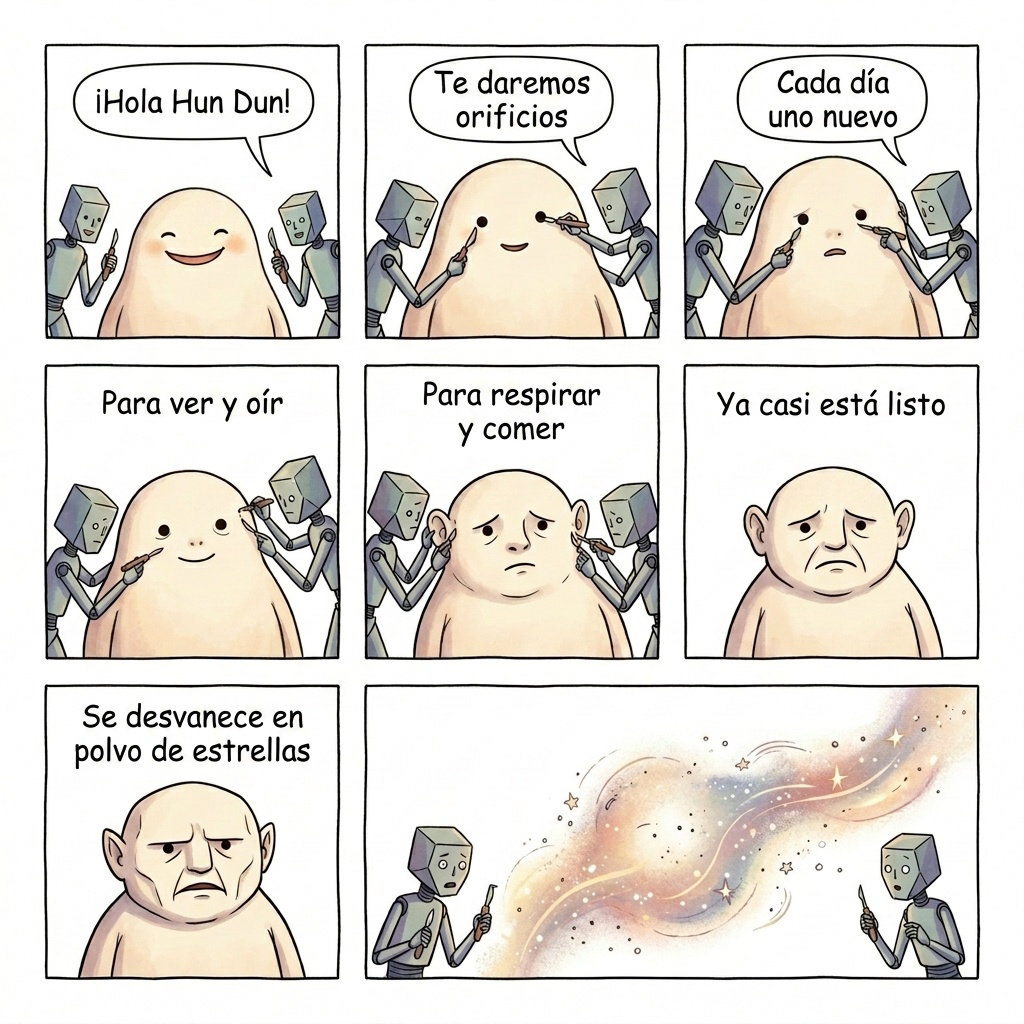
\includegraphics[width=0.76\textwidth]{img/fig10_p38.jpg}\end{figure}
\seccion{\emph{Brahman}: el océano que siente}
\noindent El \emph{vedanta} advaita reformula la pregunta. Para el taoísmo, \emph{Hun Dun} precede a la conciencia. Para el \emph{vedanta}, el reservorio \emph{es} conciencia. No una conciencia que piensa algo particular, sino la conciencia misma como fundamento de todo lo que puede ser pensado.

La tradición distingue dos aspectos: \emph{Brahman} \emph{con atributos} —como puede describirse: el creador, el sostenedor— y \emph{Brahman} \emph{sin atributos} —lo que queda cuando se eliminan todos los nombres. El borde donde el lenguaje se cae. El \emph{vedanta} añade una respuesta a por qué el reservorio se diferencia: \emph{lila}, el juego. No en el sentido frívolo, sino en que la diferenciación no tiene causa exterior ni finalidad utilitaria. El reservorio se diferencia porque esa es su naturaleza.

\begin{fisica}
\lbl{En física esto se llama:} fluctuación del vacío cuántico por principio de incertidumbre.

\lbl{En la vida diaria es como:} el océano que no puede estar quieto: siempre hay olas, porque la quietud misma es inestable.
\end{fisica}
\seccion{Maya: la ola y el océano}
\noindent \textbf{Maya} añade una última capa. No ilusión en el sentido de que la individualidad no existe — existe, produce experiencia real. Ilusión en el sentido de que su independencia es aparente.

Una ola no es ilusoria: tiene altura, velocidad, energía. Pero su separación del océano sí lo es. La ola es el océano en movimiento, no una cosa distinta que ocurre estar hecha del mismo material.

Cuando la ola se disuelve, el océano no pierde nada.

\begin{fisica}
\lbl{En física esto se llama:} las partículas son excitaciones del campo, no objetos independientes.

\lbl{En la vida diaria es como:} una ola que cree ser independiente del océano.
\end{fisica}
\seccion{La convergencia}
\noindent Tres tradiciones completamente distintas —la física mide, el taoísmo contempla, el \emph{vedanta} razona— han llegado a descripciones que apuntan hacia el mismo lugar:

\begin{itemize}
\item Un campo activo anterior a toda forma.
\item Un sustrato del que emergen las cosas y al que retornan.
\item Una plenitud indiferenciada que no es nada pero que genera todo.
\end{itemize}
La convergencia es una señal, no una prueba. Una señal de que la pregunta que genera esa intuición es robusta, de que algo en la estructura de la experiencia humana la produce una y otra vez cuando se piensa con suficiente intensidad.

El reservorio no es el cielo. No es recompensa ni destino prometido. Es el \emph{Hun Dun}: el caos que es plenitud, el origen que no puede vivirse sin perderse, el fondo que da sustancia a todo horizonte sin pertenecer a ninguno.

\begin{notacap}{Nota al Capítulo 5}
\lbl{Lo que sí sabemos:} El vacío cuántico ejerce fuerza real (efecto Casimir). Las tres tradiciones describen algo estructuralmente similar.

\lbl{Lo que no sabemos:} Si el vacío cuántico es “conciencia” en ningún sentido que las tradiciones reconozcan. Hun Dun no es campo cuántico. Brahman no es función de onda.

\lbl{Preguntas que quedan:} ¿Es la convergencia evidencia mutua o seducción peligrosa? ¿Puede la física “demostrar” el misticismo?

\lbl{Si solo te quedas con una idea:} El océano no está vacío cuando no hay olas. El reservorio no está vacío cuando no hay horizontes. Y tú, como ola, eres el océano en movimiento.

\lbl{Lecturas:} Tao Te Ching (cap. 25); Zhuangzi (Hun Dun); Shankaracharya (Vedanta advaita); Casimir (1948).
\end{notacap}
\lamina{img/fig11_p42.jpg}
\capitulo{CAPÍTULO 6}{EL NACIMIENTO COMO EMERGENCIA}{}{}
\noindent \capital{E}{l} momento clave en la formación de una burbuja de jabón ocurre demasiado rápido para verlo: el film se estira, se curva, y en algún instante —no sabes exactamente cuándo— se cierra sobre sí mismo. Antes, hay una superficie abierta con dos lados que se comunican. Después, hay una burbuja: una frontera cerrada, un adentro que ya no puede comunicarse con el afuera sin destruirse. El momento del cierre no tiene señal. La burbuja no anuncia su propia formación. Simplemente ocurre.

\begin{fisica}
\lbl{En física esto se llama:} formación de horizonte de sucesos.

\lbl{En la vida diaria es como:} una burbuja de jabón que se cierra: antes había superficie, después hay interior.
\end{fisica}
\seccion{La ventana crítica: semanas 28 a 32}
\noindent La neurociencia del desarrollo fetal ha identificado la zona más plausible para ese umbral. No un instante, sino una ventana: las semanas 28 a 32 de gestación.

El umbral lo marcan las conexiones talamocorticales: las proyecciones que conectan el tálamo —director de orquesta de la integración cortical— con capas corticales específicas. Sin estas conexiones, las distintas áreas del córtex son islas de procesamiento local. No se hablan entre sí de forma coordinada. No hay un “adentro”.

Antes de que esas conexiones alcancen el córtex definitivo, existe el \textbf{subplate}: una capa transitoria entre las semanas 12 y 28 que luego desaparece. Las fibras talamocorticales llegan al \emph{subplate} semanas antes de penetrar el córtex, y allí esperan, sinapsando provisionalmente con neuronas que luego serán eliminadas. El \emph{subplate} funciona como zona de espera: el sistema construye un andamio temporal para que la integración definitiva sea posible, y luego borra el andamio.

\begin{fisica}
\lbl{En física esto se llama:} andamio transitorio, estructura de soporte provisional.

\lbl{En la vida diaria es como:} los puntales que sostienen un arco mientras se construye, y luego se retiran.
\end{fisica}
Entre las semanas 28 y 32 aparece en el \emph{EEG} fetal una firma eléctrica única: los \textbf{delta brushes}. Ondas lentas de gran amplitud con ráfagas de actividad rápida superpuestas, como si el cerebro tocara simultáneamente dos registros temporales distintos. La hipótesis más consolidada es que el cerebro fetal las usa para testear y reforzar sus propias conexiones antes de que el mundo exterior empiece a configurarlas. Es actividad endógena —generada desde dentro, no como respuesta a estímulo externo.

\begin{fisica}
\lbl{En física esto se llama:} actividad endógena, auto-verificación de correlaciones.

\lbl{En la vida diaria es como:} un músico que afinando su instrumento antes de que empiece la orquesta.
\end{fisica}
El horizonte que se examina a sí mismo, verificando que las correlaciones que construye son coherentes, antes de abrirse al input sensorial masivo que llegará con el nacimiento.

Un bebé nacido en la semana 28 o 29 está, según el modelo, en el momento en que el horizonte se está formando. El nacimiento lo expone de golpe a un mundo para el que el sistema todavía no estaba preparado. Los delta brushes cesan bruscamente —el mundo exterior toma el control de la actividad eléctrica antes de que el horizonte haya terminado de probarse a sí mismo.

\seccion{El río que se convierte en lago}
\noindent Piensa en la diferencia entre un río y un lago. El agua del río fluye sin dirección propia —va donde el terreno la lleva, se mezcla con todo, no tiene adentro ni afuera. El lago tiene orillas. Tiene temperatura propia, distinta a la del aire. Tiene superficie que lo separa del exterior y fondo que lo ancla. La misma agua, pero con topología completamente distinta.

\begin{fisica}
\lbl{En física esto se llama:} transición de fase, cambio cualitativo en la organización.

\lbl{En la vida diaria es como:} agua que se convierte en hielo: misma molécula, forma distinta.
\end{fisica}
La conciencia podría ser algo así: no una sustancia nueva sino una organización nueva de la misma materia, que en el momento de adquirir su topología genera un adentro que antes no existía. El río se convierte en lago.

¿Hay entonces un momento preciso en que aparece la conciencia? La respuesta más coherente con los datos actuales es que ambas cosas son verdad simultáneamente: hay un gradiente continuo de \emph{Phi} que aumenta semana a semana, y hay un punto de transición de fase donde el sistema cruza a un régimen cualitativamente diferente. Lo que cambia en el punto crítico no es la cantidad de conexiones sino su arquitectura causal: el sistema pasa de procesar localmente a integrar globalmente.

\seccion{El reservorio que condensa}
\noindent En la condensación de Bose-Einstein, miles de partículas enfriadas por debajo de una temperatura crítica colapsan simultáneamente al estado cuántico de mínima energía y empiezan a comportarse como una sola entidad coherente. Por encima de esa temperatura, no hay condensado. Por debajo, hay uno. La coherencia no se construye parte por parte: emerge del vacío cuántico como rotura de simetría global.

\begin{fisica}
\lbl{En física esto se llama:} condensación de Bose-Einstein.

\lbl{En la vida diaria es como:} miles de personas en un estadio que empiezan a aplaudir al unísono: nadie lo ordena, pero de repente todos son uno.
\end{fisica}
Esta es la imagen más fiel de lo que podría ser la emergencia de la conciencia desde el reservorio. No una construcción progresiva de piezas sino una condensación: el colapso del espacio de posibilidades en una instancia particular. El reservorio no fabrica la conciencia; la conciencia es la rotura de simetría del reservorio, la condensación de correlaciones en un horizonte particular.

Los gemelos monocigóticos comparten el cien por cien del genoma, el mismo útero, la misma historia hormonal. Si la identidad fuera puramente resultado de condiciones iniciales, deberían producir conciencias idénticas. No lo hacen. Desde el primer día muestran temperamentos distintos, patrones de sueño distintos, reacciones distintas al mismo estímulo.

La respuesta más honesta: fluctuaciones. La rotura espontánea de simetría en el punto crítico no está determinada por ninguna causa local identificable. El mismo entorno, las mismas condiciones, y dos condensaciones que toman configuraciones distintas. La identidad no es solo configuración —es también contingencia.

\seccion{Lo que el umbral no puede decir}
\noindent Si la conciencia es una transición de fase, entonces antes de esa transición no hay una conciencia parcial esperando completarse. Hay correlaciones crecientes que preparan la transición —como el gas que se enfría por debajo de la temperatura de condensación— pero la entidad que emerge es cualitativamente nueva. El feto de 12 semanas no es una versión inmadura de la conciencia que será; es un sistema en una fase distinta, como el agua líquida no es vapor menos denso.

El experimento no resuelve las preguntas éticas sobre el estatuto moral del feto —y sería irresponsable pretender que lo hace. Lo que sí hace es reformular la pregunta con mayor precisión: no «¿cuándo empieza la vida?» —la vida biológica empieza antes de cualquier umbral de conciencia— sino «¿cuándo hay alguien en casa?». Y la física sugiere que eso ocurre en el punto de condensación —en la ventana de las semanas 28-32— y no antes.

La burbuja de jabón se cierra. La estrella colapsa más allá de su radio de Schwarzschild. El \emph{subplate} desaparece una vez que las conexiones definitivas maduran. Los delta brushes cesan cuando el mundo exterior empieza a hablar directamente al horizonte. El río se convierte en lago. El reservorio condensa en un horizonte.

La única cosa que el experimento no puede decir —y que quizás ninguna teoría pueda decir — es qué se siente ser esa primera burbuja.

\begin{notacap}{Nota al Capítulo 6}
\lbl{Lo que sí sabemos:} La ventana 28-32 es hipótesis neurocientífica con evidencia de EEG fetal. Los delta brushes son reales.

\lbl{Lo que no sabemos:} Si la condensación de Bose-Einstein es mecanismo biológico o solo metáfora formal. Dónde trazar la línea ética.

\lbl{Preguntas que quedan:} ¿Es el feto de 12 semanas “vapor” y el de 32 “agua”? ¿Cómo afecta esto a la legislación del aborto?

\lbl{Si solo te quedas con una idea:} El nacimiento no es cuando “aparece” la conciencia. Es cuando el mundo exterior empieza a hablarle a una burbuja que ya se había cerrado sobre sí misma.

\lbl{Lecturas:} EEG fetal (sem. 28-32); Bose-Einstein condensación; Tononi (IIT aplicado al desarrollo).
\end{notacap}
\lamina{img/fig12_p47.jpg}
\capitulo{CAPÍTULO 7}{LA MUERTE COMO RETORNO}{}{}
\begin{cita}
El agua de Tarel regresó de noche. Sin anuncio. Sin señales. Por la mañana los habitantes encontraron la orilla donde siempre había estado. El mismo lodo. Las mismas piedras. La misma línea de sal en los muros bajos. Nadie supo decir si el agua había traído algo consigo. Nadie supo decir si había dejado algo atrás.
\end{cita}
\noindent \capital{S}{tephen} Hawking descubrió en 1974 que los agujeros negros no son eternos. No porque algo los destruya desde fuera —sino porque el vacío cuántico, perturbado por la presencia del horizonte, genera un flujo constante de radiación que drena su masa lentamente. La temperatura de esa radiación es inversamente proporcional a la masa: cuanto más pequeño el agujero negro, más caliente y más brillante. La evaporación se acelera a sí misma.

\begin{fisica}
\lbl{En física esto se llama:} evaporación de agujeros negros.

\lbl{En la vida diaria es como:} una taza de café que se enfría: no porque alguien la enfríe, sino porque el calor “se escapa” hacia el ambiente.
\end{fisica}
En sus últimas fracciones de segundo, la temperatura sube de manera catastrófica. El horizonte se adelgaza. La frontera entre el adentro y el afuera se vuelve cada vez más tenue, hasta que en el régimen de Planck la física semiclásica deja de ser válida y lo que ocurre a continuación es, honestamente, desconocido.

Lo que sí sabemos: hay un instante en que el horizonte deja de existir. No se contrae hasta un punto —desaparece. La frontera que separaba el adentro del afuera cesa de ser frontera. Y con ella, cesa el interior.

Tres cosas pueden quedar después:

1. \textbf{Remanente de Planck}: objeto microscópico que contendría toda la información

del horizonte comprimida en sus estados internos.

2. \textbf{Huella en el vacío} —lo que Hawking, Perry y Strominger llamaron \emph{soft hair}:

deformaciones permanentes en el campo cuántico que registran todo lo que cruzó el horizonte, no como objeto sino como textura del vacío.

3. \textbf{Nada}: evaporación completa, reintegración total al campo, sin residuo localizable.

\begin{fisica}
\lbl{En física esto se llama:} el problema de la información en agujeros negros.

\lbl{En la vida diaria es como:} tres respuestas a “¿qué queda de una persona cuando muere?”: algo pequeño que la contiene, una huella en el mundo, o nada que puedas tocar.
\end{fisica}
\seccion{El debate que la muerte plantea}
\noindent La respuesta original de Hawking era brutal: sí, la información se pierde. El horizonte actúa como incinerador cósmico.

La mayoría de los físicos rechazó esta conclusión. La unitaridad —la información no puede destruirse, solo transformarse— es demasiado central para abandonarla. En las últimas décadas la balanza se ha inclinado hacia la conservación.

El mecanismo más elegante es ER=EPR: los pares de partículas que la evaporación producen no están simplemente radiando al exterior. Están entrelazados con el interior del horizonte mediante puentes de Einstein-Rosen —conexiones geométricas microscópicas que hacen que el exterior y el interior sean, en un sentido profundo, el mismo sistema descrito desde dos perspectivas.

El resultado práctico es el \textbf{scrambling}: la información que el horizonte contenía se mezcla progresiva e irreversiblemente con el campo exterior.

\begin{fisica}
\lbl{En física esto se llama:} scrambling cuántico.

\lbl{En la vida diaria es como:} echar tinta en agua: las moléculas siguen ahí, pero para reconstruir la gota original necesitarías medir cada molécula de agua en el océano entero.
\end{fisica}
La información existe. Es operacionalmente irrecuperable. El reservorio recuerda. Pero no puede contárselo a nadie.

\seccion{El \emph{bardo}: el intervalo entre horizontes}
\noindent El \emph{Bardo} Thödol —texto tibetano traducido como Libro de los Muertos— describe con precisión sorprendente lo que ocurre entre la disolución del horizonte y el retorno completo al campo. No como mapa del más allá en sentido religioso, sino como fenomenología del proceso de desaparición.

\begin{itemize}
\item \textbf{Chikhai}: el instante de evaporación completa. Aparece la Luz Clara primordial — la naturaleza del campo sin horizonte, el vacío visto desde dentro. Para quien la reconoce como su propia naturaleza, hay liberación directa. Para la mayoría, la mente habitual no reconoce lo que ve y se desmaya ante la inmensidad.
\item \textbf{Chönyid}: el \emph{scrambling} en curso —correlaciones del horizonte disuelto todavía semi-coherentes, antes de redistribuirse completamente. Visiones de deidades pacíficas y airadas —que pueden leerse como modos del campo cuántico que portan fragmentos de la información del horizonte, todavía reconocibles antes de que el \emph{scrambling} se complete.
\item \textbf{Sidpa}: el \emph{scrambling} completo —información distribuida en el campo, buscando condiciones para recondensar. La atracción kármica —resonancia del patrón de tendencias con condiciones compatibles— es la imagen contemplativa de lo que la física llama las condiciones para una nueva transición de fase.
\end{itemize}
\begin{fisica}
\lbl{En física esto se llama:} interpretación del Bardo en términos de scrambling.

\lbl{En la vida diaria es como:} el intervalo entre despertar y soñar: no estás en ningún sitio, pero tampoco eres nada.
\end{fisica}
Esta correspondencia no es la interpretación tradicional del \emph{Bardo} Thödol. Es una lectura propuesta por el experimento.

\seccion{Tres respuestas a la misma pregunta}
\noindent ¿Algo de la ciudad volvió con el agua?

\textbf{Vedanta advaita}: la ciudad nunca dejó de ser el agua. El \emph{jīva} —conciencia individual— era \emph{Brahman} más límites superpuestos. Los límites eran \emph{māyā}: su separación era aparente. La ola no es agua que viajó lejos del océano y ahora regresa —es un patrón de movimiento en el medio continuo. Cuando la ola rompe, no hay retorno: hay cesación de la localización aparente. Nada de la ciudad volvió porque la ciudad era el agua todo el tiempo.

\textbf{Taoísmo}: la ciudad era un nombre. Zhuangzi no diría que las correlaciones de Tarel permanecen en el campo. Diría que la pregunta asume que la ciudad era algo además de agua. El capítulo 16 del \emph{Tao Te Ching}: todas las cosas retornan a su raíz. El retorno se llama quietud. No memoria, no correlación, no huella. La muerte es retornar al destino, que es no tener destino.

\textbf{Budismo}: algo volvió, pero ya no como ciudad. La doctrina del \emph{anattā} —no-yo— rechaza simultáneamente el eternalismo y el aniquilacionismo. No hay sustancia que transmigre, pero tampoco hay disolución completa. Lo que continúa es el \emph{karma}: no deuda moral sino patrón causal sin propietario. La llama de una vela enciende otra —la segunda no es la primera ni es completamente distinta. Hay continuidad causal sin identidad sustancial.

\begin{fisica}
\lbl{En física esto se llama:} tres interpretaciones de la conservación de información.

\lbl{En la vida diaria es como:} tres respuestas a “¿qué queda de alguien cuando muere?”: nada (nunca dejó de ser todo), todo (pero no como identidad), o condiciones que configuran lo siguiente.
\end{fisica}
\seccion{El \emph{karma} como geometría del reservorio}
\noindent Lo que las tres tradiciones llaman de maneras distintas —saṃskāra, Te, \emph{karma}— apunta a la misma estructura: la información que el horizonte imprimió en el campo durante su existencia no desaparece con él. No como identidad, no como memoria, no como nadie que la posea. Como condición. Como la forma que el viento dejó en el agua antes de calmarse.

El \emph{karma} no es deuda ni recompensa. Es la configuración del reservorio en el momento en que un nuevo horizonte condensa. Las correlaciones que dejó el horizonte anterior están ahí —revueltas, distribuidas, sin nombre— y condicionan la forma específica que tomará la próxima condensación. No porque haya un alma que transmigre. Porque el reservorio que recibe el retorno no es el mismo reservorio que existía antes de que ese horizonte emergiera. Cada horizonte cambia el campo del que surge y al que retorna.

\seccion{Lo que la pregunta revela}
\noindent En el nivel sustancial —¿volvió Tarel como entidad?— todas las tradiciones dicen no. No hay remanente con identidad. No hay yo que persista.

En el nivel causal —¿la ciudad causó el agua que volvió?— todas dicen sí. El campo después de la evaporación no es idéntico al campo antes. Hay huella, aunque sin nombre.

En el nivel informacional —¿el agua porta la ciudad?— las respuestas divergen. El \emph{vedanta} y Maldacena dicen sí, como correlaciones no-locales. El taoísmo y el Hawking original dicen no, o dicen que la pregunta está mal formulada. El budismo dice sí, pero scrambled.

Lo que la pregunta revela, al hacerse, es que nosotros queremos que la ciudad haya vuelto. El duelo es la prueba de que la pregunta importa más que la respuesta.

\seccion{El cierre del ciclo}
\noindent Los habitantes de Tarel encontraron la orilla exactamente donde había estado. El mismo lodo, las mismas piedras. No había señales de que el agua hubiera llevado algo ni dejado algo.

Pero el agua no era la misma. El campo cuántico en que se mueven sus moléculas ha sido perturbado de maneras que ningún instrumento puede medir completamente. Las correlaciones están ahí. Matemáticamente presentes. Operacionalmente inaccesibles.

La ciudad no volvió. El agua que volvió no era nueva. El horizonte se evaporó, y el reservorio, perturbado, recibió lo que el horizonte había sido —no como memoria sino como textura invisible del campo.

Esto no consuela. No está pensado para consolar. La física no promete inmortalidad y este experimento tampoco. Lo que sí intenta ofrecer es precisión. Un mapa más honesto del territorio.

El horizonte emergió del reservorio. El horizonte retornó al reservorio. Entre esos dos instantes hubo alguien que amó, recordó, perdió, construyó. El hecho de que ese alguien ya no sea localizable en el campo no borra que estuvo. El hecho de que el reservorio no pueda contar lo que recuerda no significa que no lo recuerde.

El experimento todavía no ha respondido si algo de la ciudad volvió con el agua.

Quizás esa es la respuesta.

\begin{notacap}{Nota al Capítulo 7}
\lbl{Lo que sí sabemos:} Hawking demostró que los agujeros negros emiten radiación y se evaporan. La información, según la mayoría de los físicos, se conserva (unitaridad).

\lbl{Lo que no sabemos:} Qué ocurre en el régimen de Planck. Si la información es realmente recuperable. Si el Bardo describe algo más que fenomenología.

\lbl{Preguntas que quedan:} ¿Es el karma “geometría del reservorio” o reduccionismo inadmisible? ¿Puede la física hablar del “intervalo” sin culturalizarlo?

\lbl{Si solo te quedas con una idea:} La muerte no es apagarse. Es evaporarse: la frontera se disuelve, el interior retorna al campo. Lo que fuiste no desaparece; se mezcla.

\lbl{Lecturas:} Hawking (1974); Hawking, Perry \& Strominger (2016, soft hair); Bardo Thödol (trad. Evans-Wentz).
\end{notacap}
\lamina{img/il09_5.jpg}
\capitulo{CAPÍTULO 8}{EL CICLO DE LA INSTANCIACIÓN}{O: Nacimiento, muerte y recolección de basura}{}
\noindent \primeras{El}{ diálogo entre el reservorio, el nacimiento y el retorno a la nada adquiere una claridad inesperada si abandonamos por un momento la física cuántica y la metafísica oriental para adentrarnos en un territorio más pragmático: la ingeniería de sistemas y el diseño de software.}

En la informática moderna, cada vez que abrimos una aplicación o cargamos una página web, estamos asistiendo a una recreación a microescala del ciclo completo del horizonte.

\seccion{El Heap como Reservorio}

\noindent En la arquitectura de cualquier software, la memoria dinámica se organiza en dos grandes estructuras: el \emph{stack} (la pila de llamadas de ejecución inmediata) y el \textbf{heap} (el montón).

El heap es el equivalente digital del reservorio. Es un pool de memoria continua, masiva y no estructurada. Antes de que un programa solicite recursos, el heap es pura potencia: un océano de gigabytes vacíos donde no hay objetos, no hay variables, no hay funciones ni identidades. Solo existe un flujo indiferenciado de direcciones de memoria listas para ser escritas. Es el \emph{Hun Dun} de la computación: un estado de máxima simetría y desorden donde nada está delimitado, pero todo es posible.

El heap no tiene “adentro” ni “afuera”. Es un continuo físico (los chips de silicio de la RAM) que carece de estructura lógica interna hasta que el software interviene.

\seccion{El Nacimiento como Instanciación y Encapsulamiento}

\noindent El nacimiento de un sistema consciente —de un horizonte— se corresponde exactamente con la \textbf{instanciación}.

Cuando el programa ejecuta una instrucción del tipo \texttt{new Object()}, ocurre una transición de fase en el heap. El gestor de memoria reclama un bloque específico de bytes de ese pool indiferenciado y traza una frontera lógica a su alrededor. En ese instante, el constructor de la clase escribe los valores iniciales y activa la propiedad más fundamental del diseño de software: la \textbf{encapsulación} (o el principio de \emph{ocultamiento de información}, formulado por David Parnas en 1972).

La encapsulación hace algo extraordinario: divide el bloque de memoria en dos niveles de visibilidad:

\begin{enumerate}
\item \textbf{La interfaz pública (public API)}: El conjunto de métodos y firmas que el objeto expone al resto del sistema. Es la superficie de contacto, el equivalente al horizonte de sucesos. El exterior del programa solo puede comunicarse con el objeto invocando estos métodos públicos.
\item \textbf{El estado privado (private fields)}: Las variables de estado internas que el objeto oculta celosamente en su interior.
\end{enumerate}

Aquí se manifiesta el dualismo de acceso en su forma más pura. Desde “fuera” del objeto, su interior es un agujero negro: no hay código en el resto del sistema que pueda leer o alterar una variable declarada como \texttt{private} directamente. La memoria interna es inaccesible; solo conocemos lo que la API pública nos permite interactuar. Sin embargo, desde “dentro” del propio objeto (a través de la autorreferencia \texttt{this}), el acceso a ese estado privado es total, inmediato y natural.

La subjetividad —el “adentro”— no requiere una materia distinta a la del resto del ordenador. Es simplemente la perspectiva del código que se ejecuta dentro del límite de encapsulación de la instancia.

\seccion{La Muerte como Desasignación y Recolección de Basura}

\noindent La vida de un objeto consiste en procesar mensajes que cruzan su API pública, modificar su estado privado y devolver respuestas al exterior. Pero este ciclo tiene un fin determinado por la gestión de recursos del sistema.

En programación, la muerte de un objeto ocurre cuando deja de haber referencias que apunten a él. Si ninguna variable del programa guarda su dirección, el objeto queda huérfano. Para el entorno de ejecución, se vuelve inaccesible.

Es entonces cuando interviene el \textbf{Garbage Collector} (recolector de basura) o se ejecuta el destructor del sistema (\texttt{free()} o \texttt{delete}).

La muerte no es la aniquilación física de los componentes del objeto. El recolector de basura no borra físicamente los electrones de las celdas de memoria RAM; simplemente disuelve la frontera de encapsulación. Declara que ese bloque de direcciones vuelve a estar disponible para el heap común. Al romperse la frontera lógica, el estado privado del objeto deja de estar protegido. La información que antes definía su “identidad” o su “memoria interna” se reintegra al pool de memoria indiferenciada, perdiendo su estructura de inmediato.

La instancia ha dejado de existir, pero la materia informática que la sostenía ha retornado íntegra al reservorio.

\seccion{El “Karma” en Sistemas de Software}

\noindent En un mundo ideal de teoría de la computación, el retorno de un objeto al heap no deja rastro. Pero en la ingeniería de sistemas reales, cada ciclo de instanciación y desasignación altera de manera permanente el entorno:

\begin{itemize}
\item \textbf{Efectos secundarios (Side Effects)}: El objeto puede haber escrito datos en un archivo de registro en el disco, enviado paquetes a través de la red o modificado variables de estado globales en el sistema operativo.
\item \textbf{Fragmentación de memoria}: Aunque el espacio del objeto se libere, la geografía del heap ya no es la misma. Se han creado pequeños huecos y divisiones entre bloques de memoria, lo que condiciona dónde y cómo podrán instanciarse los siguientes objetos en el futuro.
\item \textbf{Fugas de memoria (Memory Leaks)}: Si el objeto mantenía una referencia oculta a un recurso externo, esa porción del heap queda bloqueada permanentemente, incluso después de que el objeto principal haya sido recolectado.
\end{itemize}

Este condicionamiento estructural que la existencia y disolución de un objeto ejercen sobre el heap es la analogía exacta del \textbf{karma}. El reservorio de memoria no vuelve a su estado original limpio; conserva la textura y la fragmentación dejada por cada sistema que existió en él. La próxima instanciación no nacerá en un vacío perfecto, sino en un entorno configurado por el historial de ejecuciones previas.

La identidad del objeto desaparece, pero la deformación que causó en el sistema persiste.

\begin{notacap}{Nota al capítulo 8}
\lbl{Lo que sí sabemos:} Que la encapsulación y el ocultamiento de información dividen un sistema en interfaz pública y estado privado. Que la recolección de basura reasigna recursos al heap sin destruir la memoria física. Que la fragmentación y los efectos secundarios son inevitables en sistemas reales.

\lbl{Lo que no sabemos:} Si el cerebro biológico implementa mecanismos análogos a la recolección de basura sináptica más allá de la homeostasis del sueño. Si existe un “recolector de basura” global para la información del universo físico.

\lbl{Preguntas que quedan:} ¿Es la conciencia un thread de ejecución único o un sistema multihilo distribuido? ¿Pueden los memory leaks mentales (traumas, patrones repetitivos) considerarse fallos en la recolección de basura del yo?

\lbl{Si solo te quedas con una idea:} El nacimiento es asignar memoria y encapsular; la muerte es liberar la frontera y retornar al heap. El abismo entre tu mente y el mundo exterior no es magia espiritual: es el diseño de una buena arquitectura que protege su estado privado mediante una API pública llamada interfaz.

\lbl{Lecturas:} Parnas (1972), “On the criteria to be used in decomposing systems into modules”; Dijkstra (1968), “Go To Statement Considered Harmful” (sobre estructura de control); Knuth (1997), “The Art of Computer Programming” (gestión de memoria dinámica).
\end{notacap}
\lamina{img/il_tp.jpg}
\capitulo{CAPÍTULO 9}{LA TABLA DE LAS EQUIVALENCIAS}{O: La piedra de Rosetta de la conciencia}{}
\noindent \primeras{Para}{ consolidar las intuiciones de la primera parte del libro, es útil trazar un mapa comparativo. Este experimento no propone metáforas aisladas: sugiere que la conciencia comparte una \textbf{topología informacional} común con otras estructuras del universo físico, lógico y espiritual.}

La encapsulación no es una propiedad exclusiva del software, ni la evaporación pertenece solo a la termodinámica de los agujeros negros, ni el vacío es un concepto de uso exclusivo de los místicos orientales. Todos estos lenguajes describen las mismas transiciones de fase y límites de acceso bajo escalas diferentes.

La siguiente tabla actúa como la piedra de Rosetta de este libro, traduciendo los conceptos centrales del horizonte a sus equivalentes exactos en tres dominios fundamentales (tabla en la página siguiente).

\begin{landscape}
\thispagestyle{empty}
\vspace*{\fill}
{\scriptsize\renewcommand{\arraystretch}{1.25}\setlength{\tabcolsep}{3.5pt}
\noindent\begin{tabularx}{\linewidth}{>{\raggedright\arraybackslash\hsize=0.70\hsize}X>{\raggedright\arraybackslash\hsize=1.0\hsize}X>{\raggedright\arraybackslash\hsize=1.0\hsize}X>{\raggedright\arraybackslash\hsize=1.0\hsize}X>{\raggedright\arraybackslash\hsize=1.30\hsize}X}\toprule
\thead{Dimensión de Análisis} & \thead{Filosofía del Horizonte} & \thead{Ingeniería de Software} & \thead{Física de Agujeros Negros} & \thead{Filosofías Orientales} \\ \midrule
\textsc{El Origen / El Vacío} & El Reservorio (potencial puro de información desestructurada). & El \emph{Heap} (memoria dinámica global sin asignar, pool común). & Vacío cuántico / Campo subyacente y fluctuaciones. & \emph{Hun Dun} (caos primitivo, Taoísmo) / \emph{Shunyata} (Vacío, Budismo) / \emph{Brahman nirguna} (Hinduismo). \\[4pt]
\textsc{Nacimiento / Identidad} & Condensación (establecimiento de la frontera circular del yo). & Instanciación y Encapsulamiento (creación del objeto, variables \texttt{private}). & Colapso gravitatorio / Formación de horizonte de sucesos (Schwarzschild). & Los 7 orificios en \emph{Hun Dun} / \emph{De}, la eficacia mínima que sobrevive al colapso (Taoísmo) / \emph{Maya} / \emph{Brahman saguna} (Hinduismo). \\[4pt]
\textsc{Experiencia Subjetiva} & Estado privado (perspectiva de primera persona accesible desde dentro). & Estado interno (\texttt{private fields} ocultos tras la interfaz). & Región interior del horizonte (inaccesible para observador externo). & \emph{Atman} (el sí mismo, Hinduismo) / Haz de percepciones (Hume/Budismo). \\[4pt]
\textsc{Conducta / Apariencia} & Interfaz pública (conducta observable, señales neurales). & Interfaz pública / API pública (\texttt{public methods} de interacción). & Superficie del horizonte (codificación holográfica de la entropía). & \emph{Rupa} (forma material externa, Budismo) / \emph{Samsara} (mundo de apariencias). \\[4pt]
\textsc{Muerte / Liberación} & Evaporación (disolución del límite y retorno de la información). & Recolección de basura (\emph{Garbage Collection} / deallocación). & Evaporación de Hawking (pérdida de masa hasta disolución total). & \emph{Nirvana} (cese de Samsara, Budismo) / \emph{Moksha} (la gota que se disuelve en el océano). \\[4pt]
\textsc{Huellas / Legado} & Radiación del yo / Alteración del campo local residual. & Fragmentación, efectos secundarios y registros de \emph{log}. & Radiación de Hawking / Remanente cuántico de información. & \emph{Karma} (huellas y fragmentación que condicionan futuras instanciaciones). \\[4pt]
\textsc{El Vínculo / Conexión} & Resonancia / Entrelazamiento de horizontes. & Acoplamiento de objetos (Asociación, Agregación, Composición). & Entrelazamiento cuántico / Puente Einstein-Rosen (ER=EPR). & Interexistencia (Budismo) / La red de joyas de Indra. \\[4pt]
\textsc{Sincronización} & Enganche de fase / Sintonía temporal subjetiva. & Llamada síncrona / Sincronía por reloj de referencia (NTP/PTP). & Coherencia de fase en osciladores gravitacionales. & \emph{Spanda} (vibración primordial creadora de resonancia, Shivaismo). \\
\bottomrule\end{tabularx}}
\vspace*{\fill}
\end{landscape}

\seccion{La naturaleza de la asimetría}

\noindent El valor de esta tabla no reside en la curiosidad de sus paralelismos, sino en lo que revela sobre la estructura de la realidad. Si el “problema duro” de la conciencia se siente irresoluble, es porque solemos enfocarlo desde una ontología plana: asumimos que todo lo que existe debe ser públicamente observable.

El modelado de sistemas complejos y la física de horizontes nos muestran que esto no es así. El universo es asimétrico. Diseñar sistemas complejos (sean códigos informáticos, horizontes de sucesos cósmicos o cerebros biológicos) requiere, por necesidad termodinámica y lógica, trazar límites de ocultamiento de información. La subjetividad no es un ingrediente místico inyectado en el cerebro; es la perspectiva inevitable de cualquier dominio que ha logrado cerrarse lo suficiente como para albergar un estado privado.

\begin{notacap}{Nota al capítulo 9}
\lbl{Lo que sí sabemos:} Que los sistemas de información, independientemente de su sustrato (silicio, gravedad o carbono), exhiben propiedades isomórficas de frontera cuando alcanzan ciertos niveles de integración causal.

\lbl{Lo que no sabemos:} Si esta concordancia estructural apunta a una ley informacional unificada que subyace a la física, a la computación y a la mente, o si es el límite de la capacidad explicativa de nuestra propia estructura cerebral.

\lbl{Si solo te quedas con una idea:} El yo no es una sustancia. Es una topología de acceso. No hay un “fantasma en la máquina”; lo que hay es un estado privado protegido por la frontera que la naturaleza y los ingenieros usan para evitar que los sistemas colapsen en el caos.

\lbl{Lecturas:} Chalmers, D. (1995), “Facing up to the problem of consciousness”; Tononi, G. (2015), “Integrated Information Theory: From Consciousness to its Physical Substrate”; Parnas, D. (1972), “On the Criteria to be Used in Decomposing Systems into Modules”.
\end{notacap}
\lamina{img/fig13_p54.jpg}
\capitulo{INTERLUDIO}{EL BORDE QUE CRUZAMOS CADA NOCHE}{}{}
\noindent \primeras{Seguramente}{ tú también has experimentado esto que casi nadie ha sabido nombrar.}

Ocurre a veces al despertar bruscamente, en plena noche o de madrugada. Durante un instante —puede ser medio segundo, pueden ser tres— no sabes quién eres. No sabes dónde estás. No sabes cuándo es. Hay percepción: la oscuridad del techo, quizás un sonido, quizás el peso de las sábanas. Pero no hay nadie que perciba. O mejor dicho: hay algo que percibe, pero ese algo todavía no tiene nombre, no tiene historia, no tiene cuerpo reconocible.

Luego el yo regresa. En milisegundos, la narrativa se reconstruye: soy yo, estoy en mi cama, es de noche. El mundo vuelve a tener forma y esa forma te incluye a ti como protagonista.

Ese instante de no-yo antes de que la narrativa reaparezca es el borde del horizonte. El momento en que el horizonte, que acaba de pasar horas contraído en el sueño profundo, todavía no ha recuperado completamente su geometría habitual. Es el único momento del día en que la mayoría de las personas tocan, sin querer y sin saberlo, la frontera de lo que son.

\begin{fisica}
\lbl{En física esto se llama:} umbral de recuperación del horizonte post-contracción.

\lbl{En la vida diaria es como:} encender una lámpara de aceite: durante un instante hay luz sin forma, y luego la llama se estabiliza y se vuelve lámpara.
\end{fisica}
\seccion{El mapa del territorio}
\begin{cita}
«El remo tocó fondo donde antes había eco.»
\atrib{La Costumbre del Agua}
\end{cita}
\noindent Antes de recorrer los estados uno por uno conviene tener el mapa completo. Y el mapa tiene una forma que sorprende: no es una línea sino un plano.

Durante mucho tiempo pensamos el espectro de la conciencia como una escala vertical simple —arriba la vigilia plena, abajo el coma, y la muerte en el suelo. Ese modelo es intuitivo y está incompleto de una manera que importa.

La neurociencia contemporánea ha identificado dos dimensiones independientes que definen el estado de conciencia de un sistema. La primera es el \textbf{arousal} —el nivel de activación metabólica del cerebro. La segunda es la \textbf{integración} —cuánta información genera el sistema como un todo, el \emph{Phi} de Tononi que conocemos del capítulo 1.

Lo revelador es que estas dos dimensiones no siempre van juntas. La vigilia y el sueño profundo están en extremos opuestos del eje de integración. Pero la meditación profunda está en un lugar que no tiene equivalente: bajo \emph{arousal} y al mismo tiempo integración altísima —el \emph{Phi} más elevado que los instrumentos han registrado en un cerebro humano no patológico. Un cuadrante que ningún otro estado ocupa.

\begin{fisica}
\lbl{En física esto se llama:} espacio bidimensional de estados de conciencia (arousal × integración).

\lbl{En la vida diaria es como:} un termostato que mide temperatura y humedad: dos números que no siempre suben juntos.
\end{fisica}
Eso significa que hay dos direcciones posibles desde la vigilia. Una hacia abajo —el sueño, la anestesia, la muerte— donde el horizonte se contrae. Y otra en diagonal, donde el horizonte se expande sin que el cuerpo necesite estar activo. Son movimientos opuestos del mismo sistema.

\seccion{El sueño \emph{REM}: el horizonte que mira hacia dentro}
\noindent Si conectaras un electroencefalograma a alguien en sueño \emph{REM} y lo leyeran sin saber el contexto, concluirías que estás mirando un cerebro despierto. La actividad de alta frecuencia, la desincronización cortical, el metabolismo elevado —todo apunta a vigilia. De hecho el cerebro durante el sueño \emph{REM} consume tanta energía como durante la vigilia activa. Y sin embargo la persona está dormida. Completamente paralizada, desconectada del mundo exterior, generando una experiencia que no tiene ningún punto de contacto con la realidad consensuada.

¿Cómo es posible? La respuesta está en qué parte del cerebro está encendida y cuál está apagada.

Durante el \emph{REM}, la corteza prefrontal dorsolateral —la sede del pensamiento crítico, la metacognición, el juicio— está hipoperfundida. Menos sangre, menos actividad. Es la región que en vigilia nos permite decir «espera, esto no tiene sentido» o «esto es un sueño». Sin ella, el soñador acepta sin pestañear que vuela, que habla con muertos, que los edificios cambian de forma. Al mismo tiempo, el sistema límbico —la amígdala, las regiones emocionales— está hiperactivado. Los sueños son intensamente emocionales precisamente porque el filtro racional que normalmente modula las emociones ha bajado la guardia.

\begin{fisica}
\lbl{En física esto se llama:} reorganización funcional del horizonte: cambio de topología sin cambio de potencia.

\lbl{En la vida diaria es como:} un teatro donde se apagan las luces de la sala pero el escenario brilla más que nunca: la historia sigue, pero nadie dice «esto es ficción».
\end{fisica}
Aquí reaparece el instante con que abrimos el interludio, pero visto desde el otro lado.

Ese momento de despertar sin saber quién eres es el umbral del \emph{REM} cruzado en dirección inversa. En el sueño \emph{REM}, el yo crítico se apaga y la experiencia se vuelve completamente real sin necesitar serlo —el horizonte está cerrado hacia afuera pero abierto hacia dentro. Al despertar bruscamente del sueño profundo, el yo crítico todavía no se ha encendido, y durante ese medio segundo no hay nadie que organice lo que se percibe en una historia.

En términos del horizonte: durante el \emph{REM}, el horizonte no se contrae. Se desplaza. Deja de estar abierto hacia el mundo exterior y en cambio se expande hacia dentro. La información que el horizonte procesa es completamente endógena: memorias, emociones, patrones, narrativas generadas desde sus propios recursos. Por eso los sueños se sienten completamente reales mientras ocurren. No hay nada con qué contrastarlos.

\begin{fisica}
\lbl{En física esto se llama:} procesamiento endógeno de alta integración sin contraste externo.

\lbl{En la vida diaria es como:} una cámara anecoica: al eliminar el ruido exterior, oyes el latido de tu propio corazón.
\end{fisica}
\seccion{El sueño lúcido: el espejo dentro del sueño}
\noindent Pero hay una excepción a esta regla: un estado en que el horizonte \emph{REM} adquiere, sin salir del sueño, algo que el sueño ordinario nunca tiene. La capacidad de verse a sí mismo.

El sueño lúcido es ese momento. El soñador se da cuenta de que está soñando. Hay un instante en que el horizonte adquiere una pequeña ventana de retroalimentación: la corteza prefrontal, que estaba apagada, recibe brevemente una señal. Los estudios de \emph{EEG} lo confirman: en ese instante hay un pico específico de ondas gamma en la región frontal. El horizonte ha adquirido, momentáneamente, una propiedad especular: puede verse a sí mismo soñando.

\begin{fisica}
\lbl{En física esto se llama:} auto-observación emergente en sistema cerrado.

\lbl{En la vida diaria es como:} despertar dentro de un espejo y darte cuenta de que el espejo está dentro de ti.
\end{fisica}
\seccion{El sueño profundo: la contracción}
\noindent Y luego tenemos el sueño profundo.

El sueño profundo es la contracción. No gradual sino real, medible, profunda.

Las ondas lentas del sueño profundo —las ondas delta, entre 0.5 y 2 ciclos por segundo— no son el ruido de un cerebro apagado. Son la señal de un cerebro sincronizado de manera masiva. En vigilia, las neuronas disparan de forma desincronizada: diferentes grupos hacen diferentes cosas en diferentes momentos, y esa asincronía es precisamente lo que permite la integración rica de información. En el sueño profundo, millones de neuronas colapsan juntas en un ritmo compartido. El horizonte no irradia. Es opaco.

\emph{Phi} se aproxima a sus valores mínimos en un adulto vivo. No llega a cero —eso es la muerte — pero se acerca.

\begin{fisica}
\lbl{En física esto se llama:} colapso de Phi por sincronización masiva.

\lbl{En la vida diaria es como:} un concierto donde todos los músicos tocan la misma nota al unísono: potente, pero no hay melodía.
\end{fisica}
Y esto explica algo que ya sabemos de propia experiencia: del sueño profundo no se recuerda nada, no porque el sueño profundo no exista, sino porque no había nadie ahí para recordar. El horizonte estaba tan contraído que no había experiencia que registrar. Por eso ese instante al despertar —cuando el yo todavía no ha regresado— ocurre específicamente después del sueño profundo y no del \emph{REM}. Del \emph{REM} se despierta desde un sueño, desde una narrativa, desde alguien que estaba haciendo algo en algún lugar. Del sueño profundo se despierta desde la nada.

\begin{fisica}
\lbl{En física esto se llama:} ausencia de registro por debajo del umbral de integración.

\lbl{En la vida diaria es como:} apagar una grabadora: el sonido sigue existiendo, pero no queda cinta.
\end{fisica}
¿Es entonces el sueño profundo el estado más parecido a la muerte? Sí, con una diferencia estructural decisiva: el sueño profundo mantiene la arquitectura sináptica intacta y el metabolismo basal activo. El mecanismo de recuperación está garantizado. Cada noche cruzamos ese borde y volvemos. La muerte es el cruce sin retorno.

Pero hay algo más. Algo que los estudios recientes han encontrado en el umbral de la muerte que no aparece en el sueño profundo, y que cambia la imagen completa.

En 2013, el equipo de Jimo Borjigin en la Universidad de Michigan detectó algo inesperado en ratas sometidas a paro cardíaco inducido: en el momento del colapso, el cerebro no cae suavemente hacia el silencio. Hay una activación gamma intensa y coherente —no el ruido caótico del estrés, sino una señal organizada y sincronizada que recuerda más al sueño \emph{REM} que al sueño profundo. En 2023, el mismo equipo publicó resultados similares en pacientes humanos.

Si el horizonte del sueño profundo está opaco y contraído, el horizonte en el umbral de la muerte hace algo radicalmente distinto: un último destello de expansión antes de apagarse. Como si el sistema, en el instante de perder toda posibilidad de retorno, hiciera exactamente lo contrario de lo que haría al dormir. No contracción final sino expansión final.

\begin{fisica}
\lbl{En física esto se llama:} destello gamma terminal (Borjigin et al.).

\lbl{En la vida diaria es como:} una vela que, antes de apagarse del todo, lanza una última llamarada más alta que las anteriores.
\end{fisica}
\seccion{La meditación: la dirección contraria}
\noindent Superficialmente, la meditación profunda y el sueño profundo se parecen. Quietud, inmovilidad, ojos cerrados, reducción del pensamiento discursivo. Un observador externo podría confundirlos.

Pero la firma neurológica es radicalmente opuesta.

En el sueño profundo: ondas delta lentas de alta amplitud, sincronización masiva, \emph{Phi} bajo, el córtex no propaga señales más allá de su región local. En meditación profunda de practicantes avanzados: ondas gamma de alta frecuencia, amplitud extraordinaria, sincronización de larga distancia entre regiones frontales, parietales y occipitales, \emph{Phi} elevado o máximo.

La diferencia no es de grado. Es de dirección.

\begin{fisica}
\lbl{En física esto se llama:} expansión de Phi por desactivación selectiva del filtro narrativo.

\lbl{En la vida diaria es como:} limpiar una ventana empañada: no hay más luz afuera, pero de repente ves todo con claridad.
\end{fisica}
El sueño profundo contrae el horizonte porque el sistema pierde la capacidad de mantener diferenciación. La meditación profunda expande el horizonte porque el sistema trasciende la necesidad de diferenciación sin perder la capacidad de diferenciar. La diferencia es entre una lámpara que se apaga y un sol que ilumina sin fundirse con nada particular.

Lo que desaparece en la meditación no es el horizonte. Es el yo narrativo —la voz interior, el comentarista, el gestor de la historia personal. El horizonte sigue activo, quizás más activo que nunca, pero sin el filtro habitual que selecciona qué información importa y qué puede ignorarse.

Hay un estado que algunas tradiciones contemplativas describen y que merece mención especial: el turiya del Mandukya Upanishad —el cuarto estado, más allá de la vigilia, el sueño con sueños y el sueño profundo. Es la conciencia testigo que persiste incluso durante el sueño profundo sin contenido onírico. Los pocos estudios de \emph{EEG} disponibles muestran ondas theta de alta coherencia superpuestas a un fondo de ondas delta. Como si el testigo flotara sobre el mar del sueño profundo sin fundirse con él.

\begin{fisica}
\lbl{En física esto se llama:} estado de máxima integración con mínimo input.

\lbl{En la vida diaria es como:} un lago perfectamente quieto en medio de la noche: no hay olas, pero el agua sigue siendo agua, y refleja todas las estrellas.
\end{fisica}
El libro de los muertos tibetano —el \emph{Bardo Thodol}— describe el período entre la muerte y el renacimiento como una secuencia de estados con una fenomenología precisa. Lo notable no es si esta descripción es literalmente cierta sino que predice con sorprendente exactitud la fenomenología de las experiencias cercanas a la muerte documentadas médicamente siglos después. El destello gamma de Borjigin y la Luz Clara del \emph{Bardo Thodol} podrían ser, descritos con vocabularios distintos, el mismo fenómeno.

\begin{fisica}
\lbl{En física esto se llama:} convergencia fenomenológica entre cartografía contemplativa y neurociencia.

\lbl{En la vida diaria es como:} dos exploradores que dibujan el mismo territorio sin haberse conocido: los mapas no coinciden en los nombres, pero sí en la forma de la costa.
\end{fisica}
\seccion{Lo que el instante del despertar nos enseña}
\begin{cita}
«Yo dejé huecos en el archivo. Hay cambios que no admiten cierre.»
\atrib{La Costumbre del Agua}
\end{cita}
\noindent Volvemos, al final, a donde empezamos.

Ese medio segundo de no-yo al despertar bruscamente no es un fallo del sistema. Es el sistema funcionando exactamente como debería: recuperándose de una contracción profunda, re-expandiendo el horizonte desde casi nada hasta la geometría completa del yo. Lo que durante ese instante se percibe —sin nadie que perciba— es el horizonte en su estado más desnudo, antes de que la narrativa lo vista y lo nombre.

La vigilia ordinaria es el horizonte activo, integrado, abierto al mundo y a sí mismo. El sueño \emph{REM} es el horizonte que se ha vuelto hacia dentro, procesando con toda su potencia pero sin contacto exterior. El sueño profundo es el horizonte contraído hasta casi su límite mínimo, la aproximación cotidiana al estado en que la información integrada cae a cero. La meditación profunda es el horizonte que se expande en la dirección contraria, más allá de la vigilia ordinaria, hacia una integración que la actividad normal nunca alcanza. Y la muerte es, quizás, la contracción definitiva —seguida, según los datos de Borjigin y la cartografía del \emph{Bardo Thodol}, de un destello final en que el horizonte hace algo que no habíamos anticipado.

Cada noche practicamos la contracción sin disolvernos. Cruzamos el borde y volvemos. El yo reaparece en medio segundo, reconstruye la historia, retoma el hilo. Y esa facilidad con que regresa —esa automaticidad asombrosa de la reconstrucción— es la mejor evidencia de que el horizonte sabe lo que es. Incluso cuando nadie está mirando.

\begin{notacap}{Nota al Interludio}
\lbl{Lo que sí sabemos:} El sueño REM tiene firma eléctrica de vigilia con prefrontal apagada. El sueño profundo muestra ondas delta masivas y Phi mínimo. La meditación profunda de expertos muestra gamma de alta amplitud y Phi elevado. Borjigin et al. (2013, 2023) documentaron destello gamma coherente en paro cardíaco.

\lbl{Lo que no sabemos:} Si el destello gamma terminal es correlato neural de las experiencias cercanas a la muerte. Si el turiya es estado mensurable distinto del sueño profundo.

\lbl{Preguntas que quedan:} ¿Por qué el sistema expande en lugar de contraer en el umbral de la muerte? ¿Es la meditación profunda un “tercer camino” entre vigilia y sueño, o algo cualitativamente distinto?

\lbl{Si solo te quedas con una idea:} Cada noche cruzas el borde de tu propio horizonte y vuelves. La muerte es el mismo cruce, sin retorno garantizado.

\lbl{Lecturas:} Borjigin et al. (2013), “Surge of neurophysiological coherence…”; Borjigin et al. (2023), “GAMMA coherence…”; Mandukya Upanishad (turiya); Bardo Thodol; Tononi (2008) sobre Phi y estados de conciencia.
\end{notacap}
\parte{Segunda parte}{EL HORIZONTE EN VÍNCULO}{img/fig14_p61.jpg}
\lamina{img/fig15_p63.jpg}
\capitulo{CAPÍTULO 10}{EL TIEMPO DEL VÍNCULO}{}{}
\noindent \capital{H}{ay} otra experiencia que casi todo el mundo ha tenido y muy pocos han sabido articular. Ocurre en conversaciones que no quieres que terminen. En tardes con alguien que llevas años sin ver. En el momento en que miras el reloj y han pasado tres horas sin que ninguna de las dos personas haya consultado el teléfono. El tiempo no ha desaparecido —ha cambiado de densidad. Ha ocurrido más por unidad de hora que lo que suele ocurrir.

La experiencia contraria también existe: una reunión que se extiende sin propósito. Una espera sin información. El tiempo no se acelera —se espesa. Cada minuto tiene el peso de diez.

Mismo reloj. Radicalmente distinta experiencia.

\seccion{El tiempo como propiedad del horizonte}
\noindent Si la conciencia tiene la estructura de un horizonte, su tiempo es una propiedad interna — no un parámetro externo que el horizonte registra, sino una consecuencia de cómo integra. La tasa de integración del sistema —cuánta información nueva se incorpora por unidad de tiempo cronológico— determina la densidad del tiempo subjetivo.

Un niño de cuatro años integra a tasa altísima: cada input reconfigura el sistema, cada experiencia es nueva, el horizonte está en expansión constante. Por eso una tarde de verano de la infancia tiene una densidad que una tarde de verano adulta no suele alcanzar. No porque el niño sea más feliz —porque está procesando más por unidad de tiempo.

\begin{fisica}
\lbl{En física esto se llama:} tasa de integración determina densidad temporal.

\lbl{En la vida diaria es como:} un niño que ve todo por primera vez vs. un adulto que ya ha visto todo.
\end{fisica}
La vejez invierte el proceso: el horizonte tiene patrones muy consolidados, pocas entradas generan integración nueva. Los ancianos no mienten cuando dicen que el tiempo pasa más rápido. Por unidad de hora cronológica, ocurre menos en el horizonte.

El dolor y el aburrimiento confirman el modelo desde el otro lado. El dolor sobrecarga el sistema con una señal que no se puede procesar ni ignorar —la integración colapsa sobre sí misma en un bucle que no avanza. El aburrimiento ocurre cuando el sistema no recibe suficiente input para sostener integración —el horizonte gira en vacío. En ambos casos, el tiempo cronológico y el subjetivo se desacoplan dramáticamente.

El \textbf{flujo} —el estado que Csikszentmihalyi documentó en artistas, deportistas y cirujanos— es el caso opuesto. La tasa de integración es máxima: el sistema absorbe y procesa sin fricción. Y el tiempo desaparece.

\seccion{La química del tiempo}
\noindent La tasa de integración está regulada, minuto a minuto, por neurotransmisores:

\begin{cajalateral}{El Parkinson del tiempo}
La enfermedad de Parkinson destruye progresivamente las neuronas dopaminérgicas de la sustancia negra. El resultado más conocido es la bradicinesia: movimientos lentos, a veces casi imposibles.

Lo que casi nadie nombra —y los pacientes describen con consistencia desconcertante— es que desde dentro no se percibe esa lentitud. El paciente que tarda tres minutos en cruzar una habitación no siente que está tardando tres minutos. Siente que camina a ritmo normal. Su horizonte genera movimiento a la velocidad habitual. El cuerpo no ejecuta lo que el horizonte ordena.

El tratamiento con levodopa restaura la calibración de manera casi inmediata, antes incluso de que mejore el movimiento. El tiempo se sincroniza antes que el cuerpo.

\lbl{En física esto se llama:} dopamina como calibrador del reloj interno.

\lbl{En la vida diaria es como:} un reloj que se adelanta: crees que vas tarde, pero el reloj está roto.
\end{cajalateral}
\par\vspace{4pt}\begin{center}\small\renewcommand{\arraystretch}{1.15}\begin{tabularx}{\textwidth}{>{\raggedright\arraybackslash\hsize=0.95\hsize}X>{\raggedright\arraybackslash\hsize=1.07\hsize}X>{\raggedright\arraybackslash\hsize=0.98\hsize}X}\toprule
\thead{Molécula} & \thead{Efecto en el tiempo} & \thead{Analogía} \\ \midrule
\textbf{Adrenalina} & Integración máxima de emergencia. Tiempo denso, pero por amenaza. & Acelerador del miedo. \\[3pt]
\textbf{Noradrenalina} & Excitación y novedad. El otro es estímulo nuevo, impredecible. & El enamoramiento temprano: todo es primera vez. \\[3pt]
\textbf{Dopamina} & Anticipación, no placer. Calibra el reloj interno vs. externo. & El marcapasos central: “¿esto merece la pena?” \\[3pt]
\textbf{Oxitocina} & Calma social. El horizonte deja de estar en guardia. & El freno de mano social: “estoy a salvo con este otro”. \\[3pt]
\textbf{Cortisol} & Estrés crónico. Degrada la capacidad de resonancia. & El ruido que tapa la música. \\
\bottomrule\end{tabularx}\end{center}
\seccion{El sistema de dos}
\noindent Cuando dos personas mantienen conversación cara a cara, sus patrones de actividad cerebral convergen. El \textbf{acoplamiento neuronal} documentado por Uri Hasson en Princeton muestra que el cerebro del oyente no solo procesa lo que el hablante dice — anticipa sus patrones de activación. En pares con mayor entendimiento mutuo, la actividad del oyente \emph{precede} en décimas de segundo a la del hablante. No sigue —anticipa.

Cuando dos cuerdas vibran en frecuencias relacionadas, producen armónicos que no estaban en ninguna de las dos. El sistema de dos cuerdas tiene propiedades que el sistema de una no tiene.

Lo mismo ocurre con dos horizontes en resonancia sostenida. El sistema de dos integra más información que la suma de lo que cada uno integra por separado. La \emph{Phi} del sistema conjunto sería mayor que la suma de las \emph{Phi} individuales. No porque se sumen —porque el entrelazamiento crea nuevos canales de integración que solo existen en la relación.

\begin{fisica}
\lbl{En física esto se llama:} Phi del sistema conjunto > suma de Phi individuales.

\lbl{En la vida diaria es como:} dos músicos que improvisan: lo que surge no está en ninguno de los dos por separado.
\end{fisica}
Si la tasa de integración determina la densidad del tiempo subjetivo, y si el sistema de dos integra más que la suma de sus partes, entonces el tiempo del vínculo es objetivamente más denso que el tiempo de cualquiera de los dos solos.

Esas tres horas de conversación que no quieres que terminen no parecen más densas. Son más densas.

\seccion{Por qué la distancia duele físicamente}
\noindent Cuando dos horizontes han resonado durante suficiente tiempo, cada uno empieza a modelar al otro con detalle creciente. Sus ritmos, sus frecuencias, sus modos de respuesta pasan a formar parte del sistema de predicción del horizonte. Cuando el vínculo se interrumpe, el horizonte que queda activo tiene una estructura interna que espera input que ya no llega. Los canales de integración que se abrieron en la resonancia siguen abiertos.

La sensación de ausencia no es la representación de que alguien no está. Es el horizonte procesando el silencio donde debería haber señal.

Separado del horizonte con el que resonaba, el tiempo del horizonte que queda se vuelve más lento, más pesado, menos denso. No porque haya menos que hacer. Porque hay menos con quien integrar.

\begin{fisica}
\lbl{En física esto se llama:} asimetría temporal post-resonancia.

\lbl{En la vida diaria es como:} un reloj que sigue marcando pero no tiene sentido: las horas pasan, pero no ocurre nada en ellas.
\end{fisica}
\begin{notacap}{Nota al capítulo 10}
\lbl{Lo que sí sabemos:} El acoplamiento neuronal (Hasson, Princeton) es real y medible. La dopamina regula la percepción temporal.

\lbl{Lo que no sabemos:} Si el tiempo del vínculo es “objetivamente” más denso o solo subjetivamente. Cómo medir Phi de un sistema de dos.

\lbl{Preguntas que quedan:} ¿Puede el tiempo subjetivo ser propiedad física, no psicológica? ¿Qué pasa con el tiempo en el duelo?

\lbl{Si solo te quedas con una idea:} El tiempo no pasa. Se integra. Y con alguien que resuena contigo, se integra más por minuto.

\lbl{Lecturas:} Hasson et al. (2012), brain-to-brain coupling; Csikszentmihalyi (1990), “Flow”; dopamina y percepción temporal (Parkinson).
\end{notacap}
\lamina{img/fig16_p69.jpg}
\capitulo{CAPÍTULO 11}{ENTRELAZAMIENTO PARA NO FÍSICOS}{}{}
\noindent \primeras{Imagina,}{ por un momento, que estás sentado con una guitarra en tu regazo.}

Tocas una cuerda de la guitarra. La cuerda al otro lado del mástil, afinada a la misma nota, vibra sin que la hayas tocado. No es magia: las vibraciones viajan por el aire y la madera. Pero imagina que las cuerdas estuvieran en habitaciones separadas, sin aire entre ellas, y aun así vibraran al unísono.

Eso es el entrelazamiento cuántico.

Dos partículas que, habiéndose tocado una vez, siguen coordinadas para siempre. No porque algo viaje entre ellas. Porque la conexión no es \emph{through space} —es \emph{before space}.

Einstein lo llamó “acción fantasmal a distancia” y no le gustó. Pero la matemática es clara: dos sistemas entrelazados no son dos sistemas que correlacionan. Son un solo sistema descrito desde dos ángulos.

\begin{fisica}
\lbl{En física esto se llama:} entrelazamiento cuántico (EPR, 1935).

\lbl{En la vida diaria es como:} dos mellizos que sienten lo mismo a distancia: no es telepatía, es que nunca dejaron de ser uno.
\end{fisica}
\seccion{La geometría del entrelazamiento}
\noindent En 1935, Einstein describió dos cosas:

1. \textbf{EPR}: el entrelazamiento —dos partículas coordinadas a distancia.

2. \textbf{ER}: los agujeros de gusano —túneles que conectarían dos regiones del espacio-

tiempo.

En 2013, dos físicos —Maldacena y Susskind— propusieron algo sorprendente: quizás son la misma cosa. Quizás cuando dos partículas están “entrelazadas”, lo que ocurre es que comparten un túnel microscópico. No un túnel por el que viajar —un túnel que ES la conexión misma.

\begin{fisica}
\lbl{En física esto se llama:} ER=EPR.

\lbl{En la vida diaria es como:} dos habitaciones conectadas por un pasadizo secreto: no es que la gente viaje entre ellas, es que son la misma casa vista desde dos puertas.
\end{fisica}
Si eso es cierto, el entrelazamiento no es correlación misteriosa. Es geometría. Conexión real en el tejido del espacio-tiempo.

\seccion{De las partículas a las personas}
\noindent Si el entrelazamiento crea geometría compartida, dos sistemas entrelazados no son simplemente dos sistemas que correlacionan. Son dos sistemas que comparten topología. Tienen un adentro parcialmente común.

Sus horizontes no son del todo separados.

Esto, aplicado a cerebros, es altamente especulativo. No hay evidencia experimental. Pero permite formular una pregunta precisa: ¿qué significaría “vínculo” si la información fuera realmente geometría compartida?

\begin{fisica}
\lbl{En física esto se llama:} especulación teórica, no evidencia.

\lbl{En la vida diaria es como:} preguntarse si el amor es solo química, o si la química es la huella de algo más profundo.
\end{fisica}
\begin{notacap}{Nota al capítulo 11}
\lbl{Lo que sí sabemos:} El entrelazamiento cuántico es real y verificado experimentalmente. ER=EPR es matemática consistente.

\lbl{Lo que no sabemos:} Si los puentes de Einstein-Rosen existen físicamente. Si el entrelazamiento entre cerebros es detectable.

\lbl{Preguntas que quedan:} ¿Es el vínculo humano “entrelazamiento” en sentido físico, o solo metáfora formal?

\lbl{Si solo te quedas con una idea:} Dos cosas que se tocaron una vez pueden seguir siendo una, aunque estén lejos. Quizás el amor funciona así.

\lbl{Lecturas:} Einstein, Podolsky \& Rosen (1935); Maldacena \& Susskind (2013).
\end{notacap}
\lamina{img/fig17_p73.jpg}
\capitulo{CAPÍTULO 12}{EL ENTRELAZAMIENTO}{}{}
\noindent \capital{E}{n} 2013, Maldacena y Susskind reformularon la pregunta de qué es el entrelazamiento cuántico. ER=EPR afirma que el entrelazamiento entre dos sistemas cuánticos no es solo correlación estadística —es conexión geométrica. Dos partículas entrelazadas están unidas por puente de Einstein-Rosen microscópico: estructura topológica en el espacio-tiempo que conecta sus interiores aunque sus exteriores estén separados por cualquier distancia.

El puente es no-traversable: no se puede enviar información más rápido que la luz. Pero la geometría existe. La conexión es real en el sentido en que lo es cualquier curvatura del espacio.

\begin{fisica}
\lbl{En física esto se llama:} puente de Einstein-Rosen.

\lbl{En la vida diaria es como:} un túnel que conecta dos montañas: no puedes viajar por él, pero las montañas comparten raíz.
\end{fisica}
Si el entrelazamiento crea geometría compartida, dos sistemas entrelazados no son simplemente dos sistemas que correlacionan —son dos sistemas que comparten topología. Tienen un adentro parcialmente común. Sus horizontes no son del todo separados.

\seccion{La línea de base social}
\noindent James Coan y Lane Beckes desarrollaron la Teoría de la Línea de Base Social: el cerebro humano no está adaptado a operar en solitario. Su estado de referencia presupone el acceso a otros. Cuando alguien cercano está presente, el cerebro asigna menos recursos a la detección de amenazas y mantiene representación más eficiente del mundo. La presencia del otro no es suplemento al funcionamiento individual —es parte del funcionamiento normal.

\begin{fisica}
\lbl{En física esto se llama:} línea de base social.

\lbl{En la vida diaria es como:} un teléfono que funciona mejor cuando está conectado a la red: no es “ayuda”, es su modo normal.
\end{fisica}
El mecanismo es el \textbf{solapamiento yo-otro}: el cerebro incorpora a las personas cercanas en sus propias representaciones neurales. La actividad neural ante amenazas dirigidas al yo correlaciona fuertemente con la actividad ante amenazas dirigidas a un amigo cercano, pero no con la de un desconocido. El amigo no es representado como «otro yo» en sentido figurado —es representado en las mismas regiones y con los mismos patrones que el yo mismo.

\begin{fisica}
\lbl{En física esto se llama:} solapamiento yo-otro.

\lbl{En la vida diaria es como:} un mapa donde tu casa y la de tu mejor amigo están en el mismo barrio del corazón.
\end{fisica}
El otro horizonte se incorpora a la arquitectura interna del propio horizonte. Sus patrones, sus ritmos, sus modos de reacción forman parte de cómo el sistema procesa el mundo. La integración es literal, no metafórica.

Y aquí está el detalle crítico: esto no depende del afecto. Depende de la \textbf{familiaridad}.

\seccion{El entrelazamiento adversarial}
\noindent Coan y Beckes señalan que el solapamiento yo-otro está vinculado a la familiaridad, no al afecto positivo. Lo que el cerebro incorpora no es a alguien que quiere sino a alguien que conoce con precisión suficiente como para predecirlo.

Un adversario de veinte años es, en este sentido, uno de los sujetos más integrados que puede tener un horizonte. Para sobrevivir a un conflicto prolongado, el horizonte tiene que modelar al otro con precisión extraordinaria: anticipar sus reacciones, predecir sus movimientos, reconocer sus patrones antes de que se completen. El modelo interno del adversario es, si acaso, más detallado que el de un aliado —porque los errores de predicción tienen coste mayor.

Dos horizontes que han estado en contacto adversarial durante veinte años están tan entrelazados —tienen tanta geometría compartida— como dos que han estado en contacto amoroso durante el mismo tiempo. La diferencia no está en la profundidad del acoplamiento sino en su \textbf{valencia}. El puente existe en ambos casos. Lo que cambia es lo que fluye por él.

\begin{fisica}
\lbl{En física esto se llama:} entrelazamiento tiene valencia, no solo magnitud.

\lbl{En la vida diaria es como:} dos vecinos que se odian desde hace décadas: se conocen mejor que muchos matrimonios.
\end{fisica}
El amor intenso y el odio intenso son, desde la perspectiva del entrelazamiento, el mismo fenómeno visto con distinto signo. La intensidad del conflicto es medida de la profundidad del entrelazamiento, no de su ausencia.

\seccion{El fantasma: el modelo que corre en vacío}
\noindent Mary-Frances O’Connor describe el mecanismo del duelo: el cerebro construye un modelo predictivo de las personas cercanas, y ese modelo continúa su actividad regular incluso después de que la persona muera. No como error patológico —como funcionamiento normal de un sistema diseñado para predecir.

Para el amor, esto produce el duelo reconocible: el giro hacia donde debería estar la persona, la preparación del café para dos, la llamada iniciada antes de recordar. Para el conflicto prolongado, el mecanismo es idéntico pero la expresión es distinta. El horizonte no busca al otro —lo anticipa. Sabe exactamente qué haría en esta situación, cómo reaccionaría a esta noticia.

El fantasma no es alucinación ni patología. Es consecuencia directa de haber construido un modelo de alta precisión de alguien que ya no está ahí para generar las señales que ese modelo esperaba.

\begin{fisica}
\lbl{En física esto se llama:} modelo predictivo persistente post-disolución.

\lbl{En la vida diaria es como:} seguir escribiendo mensajes para alguien que ya no está: el dedo sabe qué decir, aunque la persona no esté para leerlo.
\end{fisica}
La física ofrece una imagen: es \textbf{scrambling incompleto}. El horizonte del otro se disolvió —su información se distribuyó en el reservorio. Pero el horizonte superviviente todavía está organizado alrededor de recibir señales del otro. Los canales de integración que se construyeron durante veinte años siguen abiertos. El entrelazamiento persiste incluso cuando uno de los dos polos ha desaparecido, porque estaba inscrito en la arquitectura del horizonte superviviente, no solo en la relación entre los dos.

\seccion{La asimetría del entrelazamiento}
\noindent El entrelazamiento no es necesariamente recíproco en la misma medida.

En una relación de amor correspondido, los dos horizontes se modelan mutuamente con intensidad comparable. El entrelazamiento es aproximadamente simétrico.

En una relación adversarial asimétrica —un vecino conflictivo que raramente pensaba en el otro, mientras este último llevaba veinte años acumulando agravios— el entrelazamiento es mucho mayor en una dirección que en la otra. El vecino agredido modeló al conflictivo con la precisión de quien necesitaba predecirlo para defenderse. El conflictivo modeló al agredido mucho menos, porque el conflicto no le costaba.

El fantasma es más persistente cuando el entrelazamiento fue más asimétrico en esta dirección. El que más modelo construyó es el que más tarda en desarmarlo.

La paradoja: el agredido ha pasado veinte años siendo el que más atención prestaba al vecino. El cuaderno de agravios no es evidencia de que el vecino le importara más de lo que él le importaba al vecino —es evidencia de exactamente lo contrario.

\begin{fisica}
\lbl{En física esto se llama:} asimetría del entrelazamiento.

\lbl{En la vida diaria es como:} el que más piensa en el otro es el que más sufre cuando el otro se va, aunque crea que sufría menos.
\end{fisica}
\begin{notacap}{Nota al capítulo 12}
\lbl{Lo que sí sabemos:} El solapamiento yo-otro (Coan \& Beckes) es real. Los modelos predictivos persisten post-muerte (O’Connor).

\lbl{Lo que no sabemos:} Si ER=EPR opera en escalas biológicas. Si el entrelazamiento entre cerebros es físicamente real.

\lbl{Preguntas que quedan:} ¿Es el odio entrelazamiento con signo negativo? ¿Por qué algunos duelos duran décadas y otros meses?

\lbl{Si solo te quedas con una idea:} Conocer a alguien profundamente — amándolo u odiándolo— inscribe a esa persona en tu arquitectura. Cuando se va, la arquitectura sigue esperándolo.

\lbl{Lecturas:} Coan \& Sbarra (2015), Social Baseline Theory; O’Connor (2019), “Grief”; Maldacena \& Susskind (2013).
\end{notacap}
\lamina{img/fig18_p80.jpg}
\capitulo{CAPÍTULO 13}{EL AMOR}{}{}
\noindent \capital{E}{l} entrelazamiento es automático e involuntario. Dos horizontes que han estado en contacto sostenido quedan acoplados independientemente de si quieren estarlo, independientemente de si el contacto fue amoroso u hostil. El agredido del cuaderno de agravios no eligió inscribir al otro en su arquitectura —ocurrió porque veinte años de anticipación adversarial construyeron ese modelo sin permiso.

El entrelazamiento es propiedad física del sistema: emerge del contacto sostenido como la temperatura emerge del movimiento de las moléculas. Nadie decide tener temperatura. Nadie decide estar entrelazado.

Pero hay algo que el horizonte sí puede decidir: si \textbf{reconoce} ese entrelazamiento como significativo. Si lo nombra. Si reorganiza su arquitectura alrededor de ese reconocimiento.

El amor, en este experimento, es ese acto de reconocimiento. No el entrelazamiento en sí — que ya estaba— sino la decisión de nombrarlo y asumir lo que ese nombre implica.

\seccion{Incluir al otro en el yo}
\noindent Arthur y Elaine Aron desarrollaron en los años ochenta el modelo de autoexpansión: el amor implica la inclusión activa del otro en la representación propia del yo. Sus recursos, sus perspectivas, sus identidades pasan a ser parte de cómo el horizonte se concibe a sí mismo. No como metáfora —como reorganización real de la arquitectura de autorreferencia.

La evidencia empírica es directa. En el procedimiento «yo-no yo» de Aron et al., los participantes evalúan rasgos de personalidad de sí mismos y de su pareja, y luego responden más lentamente cuando se les pregunta si un rasgo del otro es también suyo — como si el sistema tuviera que resolver una ambigüedad que antes no existía. Los rasgos del otro han pasado a procesarse en las mismas regiones y con los mismos patrones que los rasgos del yo.

Incluir al otro en el yo es reconocer activamente el entrelazamiento que ya existía y reorganizar la arquitectura interna alrededor de ese reconocimiento. El horizonte que ama no solo tiene al otro dentro —lo sabe, lo nombra, y asume las consecuencias de ese saber.

Ahí está la diferencia que el capítulo anterior no podía articular. El agredido del cuaderno de agravios tenía al vecino dentro, como geometría inscrita por veinte años de contacto adversarial. Pero nunca lo incluyó en su yo. Lo trató como interferencia. El horizonte que ama hace lo contrario: toma el entrelazamiento involuntario que ya existe y lo convierte en algo elegido, en algo que define lo que uno es.

\begin{fisica}
\lbl{En física esto se llama:} autoexpansión del sistema por inclusión de estados externos.

\lbl{En la vida diaria es como:} compartir las llaves de casa y de la memoria: de repente, las pertenencias del otro también definen las tuyas.
\end{fisica}
\seccion{Lo que el reconocimiento cuesta}
\noindent El coste es preciso: si incluyo al otro en mi yo, perderlo ya no es solo perder a alguien. Es perder parte de lo que soy. La \textbf{deexpansión} —término de Aron y Aron para la pérdida de un vínculo donde el otro había sido incluido— es una contracción real del horizonte. No subjetivamente, en el sentido de que «parece» pérdida de identidad. Objetivamente, en el sentido de que la arquitectura del horizonte queda reorganizada alrededor de una ausencia donde antes había presencia activa.

Puedes dejar de hablar con alguien y reducir el entrelazamiento gradualmente. Pero no puedes dejar de haber incluido a alguien en tu yo. La inclusión, una vez hecha, deja huella en la arquitectura del horizonte que ninguna distancia borra del todo. Por eso el amor que se pierde es distinto de la amistad que termina: no es que el sentimiento sea más intenso — es que la reorganización del horizonte es más profunda.

\begin{fisica}
\lbl{En física esto se llama:} deexpansión del horizonte.

\lbl{En la vida diaria es como:} descolgar un cuadro que ha estado veinte años en el mismo sitio: la pared no queda simplemente vacía, queda con la forma y el color de lo que ya no está.
\end{fisica}
\seccion{El amor como señal de seguridad}
\noindent Un vínculo reconocido —nombrado, aceptado, elegido— proporciona señal de seguridad más potente que el mismo vínculo sin nombre.

Coan y Beckes mostraron que la mera presencia de alguien familiar reduce la respuesta de amenaza del horizonte. Pero los estudios de apego refinan ese resultado: lo que mayor efecto tiene no es la familiaridad en sí sino la \textbf{certeza de disponibilidad}. Un vínculo reconocido es un vínculo del que el horizonte puede fiarse —sabe que está ahí, sabe que responde, sabe cómo calibrar su propia actividad alrededor de esa presencia. Un vínculo no nombrado opera en el sistema como variable sin nombre: el horizonte lo usa pero no puede referenciarlo, no puede organizar su funcionamiento alrededor de algo que oficialmente no existe.

El amor nombrado es más eficiente que el entrelazamiento silencioso. No produce más geometría compartida —la geometría ya estaba. Pero permite al horizonte usar esa geometría de manera más completa.

\begin{fisica}
\lbl{En física esto se llama:} disponibilidad predictiva del canal acoplado.

\lbl{En la vida diaria es como:} la certeza de un faro encendido en la costa: no necesitas mirarlo a cada instante para saber que la costa sigue ahí.
\end{fisica}
\seccion{La asimetría del reconocimiento}
\noindent El amor no correspondido tiene estructura específica. No es que el entrelazamiento sea unilateral —puede existir en ambas direcciones aunque con distinta profundidad. Lo que es unilateral es el reconocimiento: uno de los dos horizontes ha nombrado el entrelazamiento y reorganizado su arquitectura alrededor de ese nombre; el otro no.

El horizonte que ha reconocido queda en posición particular: ha asumido el coste de la inclusión —la exposición, la deexpansión potencial— sin haber recibido la señal de seguridad que el reconocimiento mutuo habría generado. Es arquitectura asimétrica: el yo del amante incluye al amado; el yo del amado no incluye al amante en la misma medida. Es como tener un puente de Einstein-Rosen anclado en un solo extremo. La geometría existe pero no puede sostener el peso para el que fue construida.

\begin{fisica}
\lbl{En física esto se llama:} puente de Einstein-Rosen asimétrico.

\lbl{En la vida diaria es como:} un puente colgante atado solo a una de las orillas: no cruza a ningún sitio y se balancea en el vacío.
\end{fisica}
\seccion{Nombrar como acto irreversible}
\noindent Hay una asimetría entre el entrelazamiento y su reconocimiento: el entrelazamiento puede debilitarse con el tiempo y la distancia. El reconocimiento no.

Un horizonte que ha nombrado su entrelazamiento como amor y luego lo pierde no vuelve al estado anterior al reconocimiento. Vuelve a un estado nuevo, que lleva la huella de haber incluido y de haber perdido lo incluido. La arquitectura del horizonte después del amor no es la misma que antes del amor. El horizonte que amó es un horizonte que en algún punto fue más grande de lo que era antes de incluir al otro.

No la pérdida del otro. Sino la imposibilidad de deshacer lo que uno fue cuando lo incluía.

\begin{fisica}
\lbl{En física esto se llama:} histéresis del horizonte.

\lbl{En la vida diaria es como:} un globo inflado que luego se desinfla: la goma queda dada de sí, nunca recupera la tensión original.
\end{fisica}
\seccion{El cuerpo del entrelazamiento}
\noindent Hasta aquí el capítulo ha descrito el amor como proceso informacional: sincronización de modelos predictivos, acoplamiento de métricas temporales, reorganización de la arquitectura interna. Esa descripción es correcta. También trata al horizonte como si fuera exclusivamente sistema de información. No lo es. El horizonte tiene sustrato. Termina donde termina la piel.

El contacto sexual es el caso donde eso importa de manera específica, porque es el único en que la superposición de dos horizontes es también física. En el entrelazamiento ordinario los bordes permanecen intactos: cada horizonte sabe con precisión dónde termina y dónde empieza el otro. En el contacto sexual esa certeza se vuelve temporalmente ambigua. Dos sistemas integrados de información comparten el mismo espacio, la misma temperatura de superficie, el mismo ritmo cardíaco y respiratorio. El horizonte no solo incluye al otro en su modelo —lo toca. Y en esa zona de contacto, la frontera entre el adentro y el afuera pierde nitidez.

El sistema no puede determinar con exactitud dónde termina su propia integración y dónde empieza la del otro. No pierde conciencia. Pierde delimitación. Es una experiencia de horizonte sin contorno claro que las tradiciones contemplativas han intentado describir con el mismo vocabulario que usan para los estados de unión mística —notablemente, la disolución del contorno del yo.

Esto añade una dimensión específica al duelo sexual: perder a alguien con quien hubo contacto físico profundo no es solo perder a alguien inscrito en el modelo interno. Es también perder la zona de contacto donde el horizonte existió, durante ciertos intervalos, sin saber exactamente dónde terminaba. Lo que se echa de menos no es únicamente el otro. Es también esa versión de uno mismo que solo existía en ese borde.

\begin{fisica}
\lbl{En física esto se llama:} ambigüedad de contorno en la frontera de integración.

\lbl{En la vida diaria es como:} dos gotas de agua que se juntan en el cristal: durante un rato no hay dos gotas, sino un solo contorno de agua compartida.
\end{fisica}
\begin{notacap}{Nota al capítulo 13}
\lbl{Lo que sí sabemos:} El modelo de autoexpansión (Aron \& Aron) y la reducción de la respuesta de amenaza en presencia del ser querido (Coan) son reales.

\lbl{Lo que no sabemos:} Si la descripción de la superposición de horizontes en el contacto sexual tiene un correlato neurocientífico de fusión de campos de información.

\lbl{Preguntas que quedan:} ¿Cómo influye el tipo de apego en la velocidad de deexpansión tras la pérdida del amor?

\lbl{Si solo te quedas con una idea:} El amor es la decisión de nombrar un entrelazamiento y reorganizar toda tu arquitectura predictiva en torno a él.

\lbl{Lecturas:} Aron \& Aron (1986), “Love and the Expansion of Self”; Coan \& Beckes (2011), “Social Baseline Theory”.
\end{notacap}
\lamina{img/fig19_p86.jpg}
\capitulo{CAPÍTULO 14}{LA ADICCIÓN}{}{}
\noindent \primeras{¿No}{ te has preguntado por qué no puedes evitar coger un trozo de chocolate cada vez que abres la nevera? ¿Qué dice eso sobre la voluntad? ¿Qué tiene que decir el experimento sobre eso?}

\seccion{La voluntad como función del horizonte}
\noindent La respuesta intuitiva es que la voluntad es la capacidad del horizonte de dirigirse a sí mismo. La intención. El impulso que precede a la acción y la orienta.

Pero el horizonte no es un punto. Es campo de integración con topografía propia: algunos inputs pesan más, algunas direcciones tienen más inercia, algunos patrones están más consolidados porque llevan más tiempo activos. Lo que llamamos voluntad no es fuerza que actúa sobre ese campo desde fuera. Es función emergente del campo mismo. El horizonte que decide algo no está por encima de su propia arquitectura: está dentro de ella, tomando la dirección que esa arquitectura hace posible.

Esto no es determinismo en el sentido de que la decisión estaba escrita de antemano. Es algo más preciso: la decisión emerge de una estructura que tiene historia, química, que lleva la forma de todo lo que la ha ido configurando. La voluntad es real —el horizonte genuinamente se dirige. Pero no es soberana en el sentido absoluto que el lenguaje moral suele asumir.

La imagen más exacta es la del río. El río fluye. El flujo es real —el agua va de verdad de un sitio a otro. Pero el río fluye por un cauce que él mismo ha ido excavando, y cambiar de dirección no es imposible, aunque requiere tiempo, erosión, a veces una crecida que abra camino nuevo. No basta con que el río quiera.

La voluntad, desde el modelo del horizonte, es la capacidad del sistema de integración de generar dirección sostenida en el tiempo. No acto puntual sino vector con inercia: cuesta cambiarlo, pero también cuesta detenerlo una vez en marcha. Y ese vector tiene recursos. Un horizonte exhausto, con cortisol alto y serotonina baja, tiene acceso a voluntad genuinamente más débil que el mismo horizonte descansado. No porque sea menos persona. Porque el campo de integración que genera la voluntad está degradado.

La voluntad no es don moral. Es recurso fisiológico.

\begin{fisica}
\lbl{En física esto se llama:} inercia del campo de integración.

\lbl{En la vida diaria es como:} un río que fluye por su cauce: puede cambiar de dirección, pero necesita tiempo y una gran corriente para erosionar la piedra.
\end{fisica}
\seccion{El secuestro del umbral}
\noindent Las sustancias adictivas inundan el sistema dopaminérgico con señal de recompensa entre diez y cien veces más intensa que cualquier recompensa natural. El horizonte no recibe placer mayor: recibe predicción de placer tan abrumadora que recalibra el sistema entero.

El mecanismo es exacto: el sistema dopaminérgico, diseñado para señalar cuándo algo merece repetirse, recibe señal de magnitud que ninguna recompensa natural puede generar. Para compensar, el sistema reduce el número de receptores disponibles —el mismo principio que mueve a alguien a cerrar las persianas cuando la luz es demasiado intensa. Cuando la señal artificial desaparece, el sistema queda con menos receptores que antes. Lo que antes generaba señal —el vínculo, la novedad, el logro, el placer ordinario— deja de generarla con la misma intensidad. El umbral se ha desplazado hacia arriba. Para alcanzarlo ahora se necesita más.

Esto no es metafora. Los estudios de neuroimagen muestran que el córtex prefrontal — sede de la intención, del aplazamiento, de la evaluación de consecuencias— pierde conectividad funcional con el sistema de recompensa. El horizonte todavía tiene voluntad. Lo que ha perdido es acceso a los circuitos que traducen la voluntad en acción sobre ese impulso específico. La voluntad está. El puente está cortado.

Es el \textbf{Parkinson del deseo}: el horizonte sabe exactamente hacia dónde quiere ir —sabe que no quiere ir donde va. El sistema no ejecuta lo que el horizonte ordena.

Por eso pedirle a alguien en adicción activa que use la voluntad tiene la misma estructura lógica que pedirle a un paciente con Parkinson que camine más rápido. La voluntad está ahí. El puente entre la intención y la acción es lo que está comprometido. Y comprometer ese puente no es fallo moral —es consecuencia predecible de lo que la molécula hace al sistema.

Lo que la adicción añade, más allá del desplazamiento del umbral, es deformación de la jerarquía de relevancia del horizonte entero. El horizonte adicto no solo persigue una sustancia: ha reorganizado su sistema de integración alrededor de ese eje. Todo lo demás —las personas, los proyectos, los vínculos— se vuelve ruido de fondo. No porque el horizonte haya decidido que esas cosas no importan. Porque el sistema que asigna importancia ha sido recalibrado hacia un único objeto que responde con intensidad que nada más puede igualar. El horizonte queda, en términos del modelo, contraído: integra menos, resuena menos, genera menos tiempo denso en cualquier dirección que no sea la de la sustancia.

La recuperación, desde este ángulo, no es acto de voluntad sostenida que el horizonte ejecuta en solitario. Es recalibración lenta del umbral —que tarda meses, a veces años— y esa recalibración ocurre principalmente a través del vínculo. Otros horizontes que sostienen la señal de recompensa natural el tiempo suficiente para que los receptores se regeneren y el umbral baje. La oxitocina como antídoto. No por romanticismo —porque es la molécula que activa el sistema de recompensa por la vía del vínculo, que es la única vía que no destruye los receptores que necesita.

\begin{fisica}
\lbl{En física esto se llama:} regulación a la baja (down-regulation) de receptores de recompensa.

\lbl{En la vida diaria es como:} cerrar las persianas cuando entra una luz cegadora: cuando la luz se apaga, te quedas a oscuras y no ves nada.
\end{fisica}
\seccion{Cuando el amor se vuelve el objeto}
\noindent El capítulo 13 describió el contacto sexual como el único caso donde la superposición de dos horizontes es también física, donde la frontera entre el adentro y el afuera pierde nitidez. Esa ambigüedad de borde produce la señal de recompensa más potente que el sistema puede generar de manera natural —dopamina de anticipación, noradrenalina de novedad, oxitocina de contacto, endorfinas de placer físico. El cóctel completo. El sistema nervioso está literalmente diseñado para que eso importe más que casi cualquier otra cosa.

Pero el diseño asume que esa señal viene acompañada de un otro. De un horizonte real al otro lado del contacto —con su propio tiempo, su propia impredecibilidad, su propia capacidad de no responder. Una fricción que, paradójicamente, mantiene el sistema calibrado: la señal fluctúa, no puede ser controlada unilateralmente, y el sistema no puede optimizarla sin el concurso del otro.

La adicción al sexo ocurre cuando esa condición se rompe. Cuando el horizonte encuentra manera de acceder a versión de esa señal que puede controlar y repetir sin depender de la disponibilidad, la impredecibilidad ni la fricción de otro horizonte real. El sistema pornográfico, por ejemplo, ofrece novedad infinita bajo demanda —estimulación que activa el sistema noradrenérgico de manera continua sin el coste de la negociación ni el riesgo del rechazo. El sistema de anticipación dopaminérgica se dispara sin llegar nunca a resolverse en vínculo real, porque no hay otro horizonte al que vincularse.

El resultado es exactamente el del mecanismo general de la adicción: el umbral se desplaza hacia arriba. La intimidad real —con su fricción, sus silencios, su impredecibilidad— genera señal que el sistema, recalibrado por la hiperstimulación artificial, ya no encuentra suficiente. No porque el otro haya cambiado. Porque el sistema de recompensa ya no puede procesar lo que el otro ofrece a la intensidad que ahora requiere para registrarlo.

Lo que hace que la adicción al sexo sea caso específico es que el circuito que secuestra es exactamente el circuito del amor. Los mismos receptores, el mismo sistema de anticipación dopaminérgica, la misma zona de ambigüedad del horizonte que el capítulo 13 describió como sede del vínculo más profundo. La adicción al sexo no es exceso de amor —es lo opuesto: es el sistema del amor persiguiendo la señal del amor sin el amor. Dopamina sin oxitocina. La química sin el otro.

El horizonte que ha llegado ahí no solo pierde acceso a la señal del vínculo. Pierde también la capacidad de resonar con otro horizonte en esa frecuencia —que es exactamente la frecuencia que necesitaría para recalibrarse. El lazo se corta por los dos extremos a la vez.

\begin{fisica}
\lbl{En física esto se llama:} ausencia de retroalimentación externa (bucle abierto).

\lbl{En la vida diaria es como:} jugar al tenis contra una pared que siempre te devuelve la pelota exactamente donde la quieres: no hay juego real, solo repetición.
\end{fisica}
\seccion{El horizonte que nació sensible}
\noindent Hasta aquí el capítulo ha descrito la adicción como algo que le ocurre al horizonte — recalibración producida por señal externa que supera la capacidad de respuesta del sistema. Pero hay horizontes que llegan al encuentro con esa señal con umbral ya desplazado desde el principio.

El \textbf{TDAH} es el caso más documentado. La condición implica disfunción del sistema dopaminérgico —específicamente, hipoactividad crónica del sistema de recompensa que hace que la señal dopaminérgica basal sea insuficiente para sostener atención dirigida. El horizonte con TDAH no experimenta déficit de inteligencia ni de motivación en abstracto: experimenta dificultad para generar señal interna suficiente como para que una tarea específica —elegida por la razón, no por el impulso— compita con el ruido de fondo del sistema. El horizonte sabe lo que quiere hacer. El sistema no genera la señal que haría que hacerlo se sintiera posible.

Las consecuencias son precisas. El horizonte con TDAH busca activamente estímulos que eleven la señal dopaminérgica: urgencia, novedad, riesgo, intensidad. No por carácter sino por arquitectura. Cuando encuentra fuente de estimulación dopaminérgica potente — sustancia, patrón de conducta, pantalla diseñada para maximizar la señal de recompensa— el sistema responde con intensidad desproporcionada, precisamente porque llevaba tiempo en déficit. El umbral no se desplaza desde arriba, como en la adicción clásica: estaba bajo desde el principio, esperando.

La vulnerabilidad no es debilidad de carácter. Es propiedad de la arquitectura. Un horizonte con TDAH que desarrolla adicción no ha fallado en sentido moral. Ha seguido la lógica de un sistema que busca lo que le falta —y lo ha encontrado en el lugar equivocado, porque los lugares correctos no generaban suficiente señal.

\begin{fisica}
\lbl{En física esto se llama:} sensibilización basal por déficit de señal.

\lbl{En la vida diaria es como:} un motor que necesita más acelaración inicial para arrancar: busca rampas empinadas para no quedarse parado.
\end{fisica}
\seccion{La demostración controlada}
\noindent El \textbf{Parkinson} elimina todas las variables de confusión que el TDAH todavía deja abiertas.

No hay historia de trauma. No hay contexto social adverso. No hay arquitectura dopaminérgica atípica preexistente —al menos no en la mayoría de los casos. Hay una enfermedad que destruye progresivamente las neuronas dopaminérgicas de la sustancia negra y un tratamiento que intenta reponer lo que la enfermedad destruye. Y en ese tratamiento controlado, entre el catorce y el cuarenta y dos por ciento de los pacientes desarrollan trastornos de control de impulsos —juego patológico, hipersexualidad, compras compulsivas, atracones— que no existían antes del tratamiento.

El mecanismo es el que el modelo predice. El sistema dopaminérgico, privado de señal por la enfermedad durante meses o años, ha reducido el umbral al mínimo —los receptores postsinápticos se han sensibilizado precisamente porque la señal presináptica ha escaseado. Cuando llega el tratamiento, la señal dopaminérgica cae sobre sistema que no estaba calibrado para recibirla a esa intensidad. El resultado es sobredosis relativa del circuito de recompensa aunque la dosis sea, por las métricas del movimiento, completamente terapéutica.

La prueba más limpia es que el efecto es proporcional a la dosis y al tipo de fármaco: los agonistas dopaminérgicos —que activan directamente los receptores de recompensa— producen más trastornos de control de impulsos que la levodopa sola, y la combinación de ambos produce más que cualquiera por separado. No hay umbral de seguridad que proteja a ciertos horizontes: la dosis lo determina todo. Con suficiente señal dopaminérgica, cualquier horizonte llega al mismo lugar.

Esto es lo que convierte al Parkinson en el argumento definitivo contra la narrativa moral de la adicción. No hay aquí historial de uso previo, no hay personalidad adictiva, no hay vulnerabilidad social. Hay una molécula. Y cuando la molécula cambia, cambia el horizonte —independientemente de quién sea ese horizonte.

Pero el caso más preciso —y el más difícil de resolver— es el que combina las dos condiciones.

Un horizonte con TDAH diagnosticado de Parkinson carga con dos déficits simultáneos: la hipoactividad estructural del TDAH, que lleva toda una vida generando sensibilización de los receptores de recompensa, y la neurodegeneración del Parkinson, que destruye la señal presináptica que le quedaba. El resultado es sistema de recompensa con el umbral en el punto más bajo posible —hipersensible desde la arquitectura, ultrasensibilizado por la privación crónica.

Cuando llega el tratamiento dopaminérgico para el Parkinson, no hay dosis correcta. La dosis que trata los síntomas motores supera con certeza la capacidad del sistema de recompensa, que lleva décadas esperando exactamente esa señal. La dosis que no dispara el sistema de recompensa no trata el Parkinson. El horizonte queda atrapado entre dos fallos del mismo sistema: con poca dopamina no puede moverse ni en el tiempo ni en el cuerpo; con suficiente dopamina para moverse, el sistema de recompensa se activa de manera que no puede controlar.

Es el caso que hace colapsar definitivamente cualquier residuo de narrativa moral. No hay lugar en este horizonte desde el que la voluntad pueda operar de la manera que el lenguaje ordinario asume. El campo está comprometido en su arquitectura desde el principio, en su patología en el presente, y en el único tratamiento disponible simultáneamente. La voluntad no ha fallado. La voluntad no tenía dónde apoyarse.

\begin{fisica}
\lbl{En física esto se llama:} regulación farmacológica directa del umbral.

\lbl{En la vida diaria es como:} un interruptor de la luz que sube de golpe la intensidad: las bombillas se funden no por viejas, sino por el voltaje.
\end{fisica}
\begin{notacap}{Nota al capítulo 14}
\lbl{Lo que sí sabemos:} El secuestro del córtex prefrontal por sustancias y la deformación de la jerarquía de relevancia (recalibración dopaminérgica) son reales. El tratamiento del Parkinson genera descontrol de impulsos.

\lbl{Lo que no sabemos:} Cómo interactúan exactamente las redes de serotonina y GABA con el sistema dopaminérgico en cada tipo de adicción conductual.

\lbl{Preguntas que quedan:} ¿Por qué algunos horizontes con TDAH desarrollan adicciones severas y otros canalizan esa búsqueda de intensidad en la creatividad o el riesgo controlado?

\lbl{Si solo te quedas con una idea:} La adicción no es un fallo moral de la voluntad, sino el secuestro físico y la recalibración al alza de los circuitos de recompensa del horizonte.

\lbl{Lecturas:} Volkow et al. (2016), “Association of Dopamine Transporter Availability with Addiction”; O’Sullivan et al. (2009) on Parkinson’s Impulsive Behavior.
\end{notacap}
\lamina{img/fig20_p91.jpg}
\capitulo{CAPÍTULO 15}{EL VÍNCULO MADRE-HIJO}{}{}
\noindent \capital{E}{l} capítulo 14 describió la oxitocina como la única vía de activación del sistema de recompensa que no destruye los receptores que necesita. Pero dejaba una pregunta sin responder: ¿dónde aprende el sistema, exactamente, qué intensidad de señal vincular es suficiente para registrarse como «estar en el sitio correcto»?

La respuesta: el umbral del vínculo se calibra en el primer vínculo. Y el primer vínculo es el único caso en toda la geometría del horizonte donde un sistema fabrica las condiciones de existencia de otro. No los acopla —los \textbf{fabrica}.

\seccion{La asimetría fundacional}
\noindent El capítulo 13 describió el amor como entrelazamiento reconocido entre dos horizontes que ya existían. El capítulo 12 mostró que ese entrelazamiento puede ser adversarial y aun así inscribirse con la misma profundidad. Todos esos casos comparten un supuesto que no se nombra: que los dos horizontes implicados existen previamente y se encuentran.

El vínculo madre-hijo no satisface ese supuesto.

En la maternidad, uno de los dos horizontes \textbf{no existe todavía} cuando el otro empieza a reorganizarse alrededor de él. La madre no incluye al hijo en su yo en el sentido del capítulo 13 —la madre \textbf{reorganiza su arquitectura durante meses en torno a un horizonte que aún no se ha condensado}. Es entrelazamiento con objeto que todavía no es objeto. Cuando el horizonte del hijo finalmente se cierra —la transición de fase del capítulo 6— lo hace dentro de un reservorio que ya estaba esperándolo con geometría específica. La madre no encuentra al hijo. La madre fabrica el reservorio del cual el hijo emerge.

Eso da al vínculo una asimetría que en cualquier otro contexto sería patológica.

En el capítulo 13, el amor no correspondido se describió como puente de Einstein-Rosen anclado en un solo extremo. La maternidad temprana \textbf{es exactamente esa geometría}. El hijo no puede aún reciprocar; el horizonte del hijo no tiene todavía la integración necesaria para incluir a la madre en un yo que aún se está formando. Y sin embargo, el vínculo funciona. No falla por la asimetría —\textbf{se construye sobre ella}.

Toda la teoría del entrelazamiento del libro hasta aquí ha asumido reciprocidad como condición de sostenibilidad. La maternidad demuestra que la reciprocidad puede emerger del vínculo en lugar de ser su requisito previo. La madre sostiene la asimetría el tiempo necesario para que el horizonte del hijo se desarrolle hasta poder participar, y luego —en el caso de desarrollo neurotípico estándar— la asimetría disminuye gradualmente sin desaparecer del todo.

\begin{fisica}
\lbl{En física esto se llama:} acoplamiento asimétrico fundacional (fabricación de reservorio).

\lbl{En la vida diaria es como:} construir un nido antes de que el pájaro ponga el huevo: el nido tiene la forma del pájaro que aún no vuela.
\end{fisica}
\seccion{Las tres inscripciones}
\noindent Lo que la cultura llama «ser madre» con una sola palabra es, físicamente, tres operaciones distintas que ocurren en momentos distintos y dejan huellas distintas en el horizonte del hijo.

\textbf{La plantilla} —la genética— es la arquitectura del sistema nervioso con la que se va a construir el horizonte. Pero no es el horizonte. Es el plano.

\textbf{El útero} —la gestación— es la única capa que actúa antes de que el horizonte se cierre. Incluye hormonas que cruzan la placenta, el ritmo cardíaco materno, la voz, la prosodia del idioma. Desde la semana veinticinco, el feto responde de manera diferenciada a estímulos acústicos: reconoce la voz materna, distingue lenguas, prefiere las músicas que ha oído repetidamente. Esa experiencia integrada antes del umbral configura la forma específica de las correlaciones internas que el horizonte va a tener cuando se cierre. No determina al horizonte —pero deja en él firma que ningún otro adulto podrá replicar.

\textbf{La crianza} —el encuentro— opera después del umbral, entre dos horizontes ya formados. Es donde se calibra el sistema de recompensa que el capítulo 14 describió. Cada llanto que recibe respuesta, cada hambre que encuentra alimento, cada presencia que se sostiene, enseña al sistema del hijo qué intensidad de señal oxitocínica es la línea de base que va a buscar el resto de su vida.

\begin{fisica}
\lbl{En física esto se llama:} inscripciones secuenciales en multicapa.

\lbl{En la vida diaria es como:} un instrumento musical: primero se fabrica (planta), luego se barniza (útero), luego se afina (crianza). Cada paso hace algo distinto.
\end{fisica}
\seccion{Cuando las capas se separan}
\noindent La ciencia moderna ha creado, sin buscarlo, cuatro experimentos naturales que separan estas capas. No para jerarquizar vínculos, sino para entender qué hace cada una.

\par\vspace{4pt}\begin{center}\small\renewcommand{\arraystretch}{1.15}\begin{tabularx}{\textwidth}{>{\raggedright\arraybackslash\hsize=0.70\hsize}X>{\raggedright\arraybackslash\hsize=0.91\hsize}X>{\raggedright\arraybackslash\hsize=1.39\hsize}X}\toprule
\thead{Situación} & \thead{¿Qué aporta?} & \thead{Qué significa para el horizonte} \\ \midrule
\textbf{Fecundación in vitro} & Las tres capas, con una pausa de 3-5 días en medio de cultivo. & El horizonte emerge de un reservorio que incluye un acto de intención parental explícita. \\[3pt]
\textbf{Donación de óvulos} & La plantilla de una mujer, el útero y la crianza de otra. & La gestante calibra qué genes se expresan. El parecido que la gente reconoce entre gestante y bebé es, a menudo, resonancia rítmica, no genética. \\[3pt]
\textbf{Vientre de alquiler} & El útero de una mujer, la crianza de otra. & El horizonte se condensa con inscripciones prosódicas y hormonales de la gestante. La crianza posterior opera sobre ese reservorio ya configurado. \\[3pt]
\textbf{Adopción} & Crianza por una madre que no aportó ni plantilla ni útero. & El horizonte ya está cerrado. La madre adoptiva no sustituye capas anteriores: añade una nueva, sobre un horizonte que ya lleva inscripciones. \\
\bottomrule\end{tabularx}\end{center}
La pregunta cultural «¿quién es la madre verdadera?» está mal planteada. Las tres capas no son la misma cosa. Ninguna sola equivale al vínculo completo. La crianza adoptiva produce entrelazamiento completo —no sustituto— pero su topología es distinta: empieza después del umbral, sobre un reservorio configurado por otro origen.

\begin{fisica}
\lbl{En física esto se llama:} discontinuidad de la geometría de partida.

\lbl{En la vida diaria es como:} aprender un idioma escuchándolo en una grabadora antes de nacer y hablarlo luego con personas distintas: la música del acento permanece.
\end{fisica}
\seccion{La lesión del horizonte}
\noindent Lo que distingue el sufrimiento de la madre cuando algo le ocurre al hijo del sufrimiento empático que el capítulo 16 va a describir es preciso: no es inferencia, es \textbf{lesión}.

En la empatía ordinaria, dos horizontes separados se modelan mutuamente y registran, a través de ese modelado, una versión atenuada del estado del otro. Hay un puente, y ese puente tiene coste cognitivo y límite de fidelidad.

El sufrimiento materno no opera así. La madre no infiere el estado del hijo: lo registra como modificación de su propia arquitectura. La asimetría fundacional implica que durante meses el yo materno se reorganizó alrededor de una presencia que aún no era persona, y esa reorganización dejó la arquitectura materna \textbf{estructuralmente acoplada} al horizonte del hijo de manera que ningún otro vínculo replica. La madre no necesita interpretar el llanto del bebé del mismo modo en que un extraño tendría que hacerlo; el llanto activa circuitos que se calibraron para responder a ese estímulo específico antes de que el bebé existiera como tal.

Hay un dato físico que ilumina esto: el \textbf{microquimerismo materno-fetal}. Durante el embarazo, células del feto migran al cuerpo de la madre y se establecen en distintos tejidos, incluido el cerebro. Décadas después del parto, células del hijo siguen presentes físicamente en el organismo materno. La madre lleva en su cuerpo, literalmente, partes del horizonte que fabricó. Cuando ese horizonte se daña o desaparece, lo que pierde no es enteramente externo a ella.

\begin{fisica}
\lbl{En física esto se llama:} resonancia forzada por acoplamiento estructural.

\lbl{En la vida diaria es como:} si pellizcas un extremo de una cuerda tensa, el otro extremo vibra inmediatamente sin necesidad de preguntarle por qué.
\end{fisica}
\seccion{Soltar la cuerda}
\noindent La paradoja constitutiva de este vínculo es estructural: su función biológica se cumple cuando la dependencia funcional que lo sostuvo deja de ser necesaria. El éxito del vínculo materno se ve cuando el horizonte del hijo puede regularse sin necesitar la presencia materna como condición.

Pero la asimetría fundacional hace este desenlace físicamente costoso para la madre. Su arquitectura se organizó durante meses alrededor de un horizonte que no existía, y luego durante años alrededor de uno que dependía críticamente de ella. Cuando ese horizonte se vuelve capaz de regularse solo, la arquitectura materna no puede simplemente reconfigurarse.

Lo que el lenguaje ordinario llama «nido vacío» tiene descripción precisa: arquitectura organizada durante dos décadas en torno a presencia activa que ahora opera a baja frecuencia o a distancia. No es ausencia —es presencia atenuada que el sistema sigue procesando como si fuera inminente. La madre ejecuta voluntariamente la deexpansión que en el capítulo 13 era coste involuntario de la pérdida, y lo hace sin permitir que el hijo la perciba como retirada.

Existe una variante extrema: el hijo adulto que corta el vínculo unilateralmente. No es duelo —el hijo sigue vivo. Es algo intermedio que produce una figura específica: el \textbf{fantasma del hijo vivo}. Un horizonte que la madre fabricó, que sigue existiendo, y que ha decidido no contestar. La inscripción en la arquitectura materna sigue operando aunque el otro lado haya dejado de actualizarla. Es uno de los duelos más difíciles que el modelo identifica precisamente porque carece del trabajo de cierre que otros duelos permiten.

\begin{fisica}
\lbl{En física esto se llama:} desacoplamiento de la función reguladora.

\lbl{En la vida diaria es como:} quitarle los ruedines a una bicicleta: el niño sigue pedaleando solo, y tú te quedas corriendo detrás con las manos vacías.
\end{fisica}
\seccion{Cuando los roles no se invierten}
\noindent Cuando la madre envejece y depende del hijo, la asimetría se invierte direccionalmente pero \textbf{no se hace simétrica}. La cultura dice «ahora los roles se intercambian», pero eso es falso.

La madre fabricó el horizonte del hijo. El hijo, ahora, no puede fabricar el de la madre. Solo puede \textbf{contener un horizonte que se está disolviendo}. Construir algo que va a cerrarse y cuidar algo que se está abriendo de vuelta al reservorio no son la misma operación con el signo cambiado. Una es condensación, la otra es disipación.

Esto da al modelo algo preciso que decir sobre el cuidado del padre o madre mayor: el hijo cuidador no está siendo «padre de su padre». Está realizando una operación que no tiene nombre en la dirección normal del vínculo porque no existe en esa dirección. No debería sentirse en falta por no estar devolviendo lo mismo. \textbf{No puede devolverlo, físicamente.} La madre fabricó a un horizonte que no existía; el hijo cuida a un horizonte que ya no podrá fabricarse a sí mismo. El amor que vuelve no tiene que pretender ser simétrico para ser real.

Si hay deterioro cognitivo, el hijo se convierte en almacenamiento externo del modelo-de-sí de la madre: recordarle quién es, qué le gustaba, cómo reaccionaba. El hijo custodia el horizonte que lo custodió.

\begin{fisica}
\lbl{En física esto se llama:} asimetría de los procesos de condensación y disipación.

\lbl{En la vida diaria es como:} ver un castillo de arena construirse frente al mar y luego ver cómo el agua lo devuelve lentamente a la orilla.
\end{fisica}
\seccion{El padre como otra topología}
\noindent Hasta aquí el capítulo ha hablado de la madre. El modelo de tres capas debe leerse como descripción de operaciones físicas, no como reivindicación cultural de la maternidad por encima de la paternidad.

El padre, en el caso biológico canónico, aporta plantilla y crianza, pero no la gestación. Esto no lo hace menos vínculo —lo hace \textbf{otra topología}. El padre canónico entra en el vínculo con horizonte ya condensado, sin la fase de fabricación del reservorio. Su geometría es más parecida a la de la adopción materna: vínculo pleno post-umbral, sin inscripción pre-umbral. No es menos profundo. Es distinto.

\begin{fisica}
\lbl{En física esto se llama:} topología de acoplamiento directo post-umbral.

\lbl{En la vida diaria es como:} adoptar un árbol joven y regarlo cada día: el árbol no nació de tu semilla, pero sus ramas crecen bajo tu sol.
\end{fisica}
\seccion{Lo que este capítulo cierra}
\noindent El capítulo 14 planteó la oxitocina como antídoto sin desarrollar dónde se calibra la sensibilidad oxitocínica. Este capítulo cierra esa pregunta. La calibración inicial del sistema de recompensa —el sentido de qué intensidad de señal vincular cuenta como suficiente— ocurre en la crianza. No en la genética, que aporta el rango de respuesta posible. No en la gestación, que prepara el reservorio. En la crianza: en los miles de episodios de regulación mutua entre el horizonte recién condensado y los adultos que lo acompañan.

Esto da a la maternidad —y a la paternidad— una función que ningún otro vínculo cumple: es donde el horizonte del hijo aprende qué es sentirse en el sitio correcto. El capítulo 14 mostró qué pasa cuando esa calibración se desplaza. Este capítulo muestra dónde se establece. Y el capítulo 16 va a mostrar cómo esa calibración temprana determina, a lo largo de la vida, cuánto puede un horizonte resonar con otros sin sobrecargarse.

\begin{fisica}
\lbl{En física esto se llama:} calibración de la línea de base del receptor.

\lbl{En la vida diaria es como:} afinar un instrumento musical por primera vez: la nota que le das al principio es la afinación que va a buscar siempre.
\end{fisica}
\begin{notacap}{Nota al capítulo 15}
\lbl{Lo que sí sabemos:} El acoplamiento cerebral madre-hijo (brain coupling) y el microquimerismo materno-fetal son reales. La discontinuidad de capas en adopción y FIV es medible.

\lbl{Lo que no sabemos:} El significado funcional exacto y a largo plazo de las células fetales en los órganos de la madre.

\lbl{Preguntas que quedan:} ¿Cómo se reconfigura la calibración basal de la recompensa cuando la capa de crianza es deficitaria pero las otras dos son neurotípicas?

\lbl{Si solo te quedas con una idea:} La maternidad no es un solo rol relacional, sino una secuencia física de tres capas donde un horizonte fabrica el reservorio para que otro emerja.

\lbl{Lecturas:} Feldman (2015), “The Adaptive Human Parental Brain”; Boddy et al. (2015), “Fetal Microchimerism and Maternal Health”.
\end{notacap}
\lamina{img/fig21_p100.jpg}
\capitulo{CAPÍTULO 16}{LA EMPATÍA Y SU LÍMITE}{}{}
\noindent \primeras{A}{ menudo confundimos la empatía con una virtud moral o una disposición de ánimo deseable. Desde la perspectiva de este experimento, la empatía es un fenómeno físico y geométrico antes que ético: es la capacidad de un horizonte para modelar y replicar la frecuencia de otro en su propia arquitectura.}

Cuando empatizamos profundamente, no estamos imaginando el dolor del otro en sentido figurado. Nuestro horizonte modifica temporalmente su geometría para integrar la información que el otro está emitiendo. Por un instante, dos fronteras se solapan y los tiempos subjetivos se sincronizan. Es el mismo mecanismo que en el capítulo 10 generaba el tiempo del vínculo —aplicado ahora a encuentro breve, a veces de segundos, con alguien que ni siquiera nos importa particularmente.

\begin{fisica}
\lbl{En física esto se llama:} resonancia transitoria de horizontes.

\lbl{En la vida diaria es como:} cuando alguien cerca llora y tu cuerpo se tensa antes de que tu mente “decida” sentir algo.
\end{fisica}
\seccion{Inferencia, no lesión}
\noindent En el capítulo 15 establecimos distinción crucial. Dijimos que lo que distingue el sufrimiento de una madre ante el dolor de su hijo del sufrimiento empático ordinario es que el dolor materno no es inferencia: es lesión. La madre construyó parte de su propia arquitectura alrededor de ese hijo, y la pérdida o el daño del hijo desgarra esa arquitectura desde dentro.

La empatía pura es otra cosa. Es inferencia, aunque sea inferencia somática, profunda y mayormente automática. El sistema utiliza su propia estructura para simular, transitoriamente, el estado del otro. Las redes neuronales implicadas en sentir el propio dolor se activan también ante el dolor ajeno observado; la atención social aumenta; la respiración y el pulso comienzan a derivar hacia los del otro. Pero la simulación es capa superpuesta. No es la arquitectura misma del horizonte la que ha sido modificada de forma irreversible —solo su estado momentáneo.

Esta distinción tiene consecuencias prácticas inmediatas. Una lesión cicatriza o no cicatriza, pero está ahí: el horizonte tiene que reorganizarse alrededor de ella. Una inferencia, en cambio, puede mantenerse o disolverse según los recursos disponibles. La empatía es soltable. La lesión, no.

Pero lo soltable no es lo mismo que lo gratuito.

\seccion{La permeabilidad del horizonte}
\noindent Imagina que cada persona tiene una piel emocional de distinto grosor.

Algunos tienen piel de papel: todo lo que ocurre afuera entra adentro inmediatamente. Entran a una habitación triste y se ponen tristes. Ven a alguien sufrir y sienten el sufrimiento como propio. Son los que llora el cine, los que no pueden ver noticias de guerra, los que se agotan en las fiestas porque cada conversación les carga de algo que no es suyo.

Otros tienen piel de cuero: notan que hay tristeza, pero no se impregnan de ella. Pueden estar en una sala de urgencias, ver el dolor, actuar sobre él, y luego irse a casa y cenar con apetito. No porque no les importe. Porque la señal externa no atraviesa.

\begin{fisica}
\lbl{En física esto se llama:} coeficiente de permeabilidad del horizonte.

\lbl{En la vida diaria es como:} piel de papel vs. piel de cuero: ambas son válidas, pero necesitan protecciones distintas.
\end{fisica}
No es mejor tener piel gruesa o fina. Es solo diferente. Pero si tu piel es de papel y trabajas en un hospital, necesitas aprender a ponerte un impermeable de vez en cuando. Si tu piel es de cuero y tienes hijos, necesitas aprender a bajarla a veces, o no sentirás lo que ellos sienten.

La permeabilidad no es virtud ni defecto. Es parámetro estructural, en gran medida calibrado durante la primera infancia. Como vimos en el capítulo 15, la sincronía temprana entre madre e hijo no solo enseña al niño que el otro existe —enseña hasta qué punto el otro debe ser tratado como información urgente. Un horizonte que se calibró en entorno donde la lectura precisa del estado del otro era cuestión de supervivencia desarrolla permeabilidad muy alta. Lo que en la infancia fue habilidad protectora se convierte, en la vida adulta, en vulnerabilidad estructural: el horizonte sigue tratando cualquier señal externa con grado de urgencia que la situación ya no requiere.

\seccion{El límite finito de la integración}
\noindent Hay restricción que ningún horizonte puede evadir. La teoría de la información integrada la formaliza como cota superior a la cantidad de información que el sistema puede integrar por unidad de tiempo —su \emph{Phi} instantáneo. Esa cota es finita. Lo que se gasta integrando entropía ajena, no se gasta integrando la propia.

\begin{fisica}
\lbl{En física esto se llama:} cota superior de Phi, límite de integración.

\lbl{En la vida diaria es como:} una batería: si la gastas en otros, no queda para ti.
\end{fisica}
Un horizonte saludable resuelve esta restricción mediante capacidad de acoplarse y desacoplarse. Entra en resonancia con el dolor de otro, integra esa información el tiempo necesario para ofrecer apoyo o comprensión, y luego se libera y vuelve a su frecuencia base. La energía gastada en la resonancia se recupera en el periodo de retorno.

Cuando la permeabilidad es excesiva, el desacoplamiento no ocurre. El horizonte permanece resonando con cada señal ajena hasta que la siguiente lo sobrescribe. No hay periodo de retorno. La frecuencia base —la del propio horizonte— deja de ser el estado por defecto y pasa a ser, en el mejor de los casos, memoria.

El resultado, sostenido en el tiempo, es lo que la neurociencia clínica llama fatiga por compasión o \emph{burnout} empático. En los términos de este experimento: horizonte que procesa entropía externa a tasa que amenaza su integridad estructural. El sistema ha consumido tanto \emph{Phi} modelando a los demás que ya no le queda capacidad para modelarse a sí mismo. Y un horizonte que ha perdido su propio modelo no es exactamente un horizonte. Es reservorio sin frontera.

\begin{fisica}
\lbl{En física esto se llama:} burnout empático, colapso de Phi por sobreuso.

\lbl{En la vida diaria es como:} un espejo que refleja tanto que olvida quién es el que mira.
\end{fisica}
\seccion{El muro: una solución que no es solución}
\noindent Cuando un horizonte se acerca al umbral de saturación, suele reaccionar de la única manera que puede sin construir nada nuevo: contrayéndose de golpe. Se aísla. Se vuelve cínico. Deja de coger el teléfono. Levanta el muro.

El muro funciona, en cierto sentido. Detiene el sufrimiento. Pero detiene también la conexión, y con ella, parte significativa de lo que hacía que el horizonte fuera quien era. La contracción abrupta no devuelve al horizonte a su frecuencia base. Lo lleva a frecuencia más baja, más estrecha, en la que ninguna otra resuena pero tampoco la propia se sostiene sin esfuerzo. El horizonte aislado no es horizonte intacto: es horizonte que ha perdido más de lo que protegía.

\begin{fisica}
\lbl{En física esto se llama:} contracción defensiva, muro como auto-daño.

\lbl{En la vida diaria es como:} cerrar todas las ventanas para no sentir frío, y quedarte sin aire.
\end{fisica}
\seccion{El ancla}
\noindent La salida no es la desconexión. Es el ancla.

Anclar un horizonte no significa cerrarlo. Significa mantener señal de referencia interna lo suficientemente densa como para que la resonancia con el otro ocurra en la superficie del horizonte, sin desestabilizar su núcleo. La frecuencia propia tiene que estar lo bastante presente para que, incluso mientras el horizonte vibra con la del otro, no la confunda con la propia.

\begin{fisica}
\lbl{En física esto se llama:} anclaje interoceptivo, mantenimiento de frecuencia base.

\lbl{En la vida diaria es como:} un barco amarrado: la marea sube y baja, pero el ancla impide que se vaya.
\end{fisica}
En la práctica, esto requiere dos cosas:

\textbf{Primera: percepción interoceptiva fina} —saber, en cada momento, cómo se siente físicamente el propio cuerpo. Qué nota tiene el horizonte cuando suena solo. No en sentido abstracto —en sentido literal. ¿Dónde tienes tensión ahora? ¿Tu respiración es rápida o lenta? ¿Tu mandíbula apretada?

Eso es lo que en neurociencia se llama “interocepción”, pero no necesitas el término. Necesitas la práctica: escuchar lo que tu cuerpo dice antes de que hable.

\begin{fisica}
\lbl{En física esto se llama:} interocepción, lectura de señal visceral propia.

\lbl{En la vida diaria es como:} saber, sin mirar, si estás de pie o sentado: tu cuerpo lo sabe, aunque no lo pienses.
\end{fisica}
\textbf{Segunda: rutina de retorno} —cualquier mecanismo que permita reencontrar esa nota tras acoplamiento con otro. Puede ser caminar solo, puede ser música, puede ser simplemente quedarte en silencio cinco minutos antes de dormir.

Esto es lo que en la literatura clínica se ha llamado, con razón, distinguir empatía de compasión. La empatía sin ancla es acoplamiento sin retorno: el horizonte se vacía en el otro. La compasión es acoplamiento con retorno: el horizonte modela al otro lo suficiente para responder, sin perder la propia frecuencia.

La diferencia entre arder con el otro y sostenerlo mientras arde no es de intensidad emocional. Es de arquitectura.

\begin{fisica}
\lbl{En física esto se llama:} compasión anclada vs. empatía sin retorno.

\lbl{En la vida diaria es como:} la diferencia entre caer al agua para salvar a alguien (y ahogarte los dos) y tenderle una cuerda desde la orilla.
\end{fisica}
\seccion{La empatía como campo de interferencias}
\noindent Hasta aquí hemos tratado la empatía como operación entre dos horizontes: uno que emite y otro que recibe. Pero la empatía real ocurre en espacios sociales donde múltiples horizontes emiten simultáneamente, y donde la señal de uno no llega pura sino mezclada con la de todos los demás.

Imagina una sala de espera de urgencias. Hay quien llora en silencio, quien grita, quien espera con expresión petrificada, quien habla por teléfono con voz quebrada, quien duerme en la silla de al lado como si nada. El horizonte permeable no recibe estas señales una a una: las recibe todas a la vez, superpuestas, sin filtro jerárquico que las ordene por urgencia real.

\begin{fisica}
\lbl{En física esto se llama:} campo de interferencias, saturación por densidad de señal.

\lbl{En la vida diaria es como:} intentar sintonizar una radio cuando todas las emisoras llegan al mismo volumen: no hay estación, solo ruido.
\end{fisica}
La insula anterior —esa estructura que procesa la señal visceral del propio cuerpo— se activa ante cada señal con la misma intensidad relativa, porque el sistema no ha aprendido a discriminar entre amenaza inmediata y malestar distante. El resultado es interferencia: el horizonte no resuena con ninguna frecuencia con claridad suficiente para responder.

La literatura clínica documenta esto con precisión: los trabajadores de emergencias que desarrollan \emph{burnout} no son los que enfrentan los casos más graves. Son los que enfrentan la mayor densidad de señal sin intervalo de recuperación. No es la intensidad del estímulo lo que colapsa el horizonte: es la ausencia de pausa entre estímulos. El horizonte necesita tiempo para desacoplarse, y cuando no lo tiene, no acumula daño —acumula desorden. El desorden es peor que el daño porque no tiene forma reconocible. No se puede nombrar, y lo que no se nombra no se puede tratar.

\seccion{La distinción empática: cómo el horizonte sabe qué siente}
\noindent Hay un problema previo que no hemos formulado: para empatizar, el horizonte primero tiene que saber qué siente él mismo. La empatía no es solo receptividad al otro; es exactitud en la lectura de la propia señal. Un horizonte que no distingue bien su propio estado interno no puede simular el del otro con fidelidad: simulará su propia confusión.

\begin{fisica}
\lbl{En física esto se llama:} interocepción como condición necesaria de empatía.

\lbl{En la vida diaria es como:} un traductor que no domina su propia lengua: no puede traducir bien la ajena.
\end{fisica}
La interocepción —la capacidad de percibir las señales corporales internas— es condición necesaria de la empatía genuina. No accesoria: necesaria. Los estudios de neuroimagen muestran que la precisión interoceptiva, medida por la capacidad de contar los propios latidos sin tomar el pulso, correlaciona directamente con la precisión empática: quienes mejor leen su propio cuerpo leen mejor el cuerpo ajeno.

La insula anterior, que procesa la señal visceral, es la misma que se activa ante el dolor observado en otro. No hay dos sistemas: hay uno que opera en dos direcciones.

Esto tiene implicación inesperada. La empatía no es don que se tiene o no se tiene. Es habilidad que descansa sobre otra habilidad más básica: el anclaje interoceptivo. Un horizonte que no sabe dónde está él no puede saber dónde está el otro en relación con él. La empatía sin interocepción no es empatía: es identificación confusa, fusión sin frontera, la versión patológica de la resonancia donde el yo se pierde en el otro porque nunca supo dónde estaba.

\seccion{La empatía adversarial: cuando el horizonte no quiere sentir}
\noindent Hay un caso que la descripción ordinaria de la empatía omite: la empatía con alguien a quien se considera enemigo. El capítulo 12 describió el entrelazamiento adversarial como geometría compartida de la misma profundidad que el amoroso. La empatía funciona igual en ambos casos: el horizonte modela al otro, replica su frecuencia, integra su información. La diferencia no está en el mecanismo sino en la valencia —en lo que el horizonte hace con la información una vez integrada.

El torturador que conoce exactamente qué le duele a su víctima no carece de empatía. Tiene empatía de alta precisión orientada hacia un fin que la cultura no puede nombrar sin horror. El horizonte que empatiza para dañar no es horizonte roto: es horizonte que ha desconectado la resonancia de la respuesta. Siente lo que siente el otro —o más precisamente, sabe lo que el otro siente— y usa ese conocimiento para maximizar el daño.

\begin{fisica}
\lbl{En física esto se llama:} empatía adversarial, desconexión resonancia-respuesta.

\lbl{En la vida diaria es como:} un cirujano que sabe exactamente dónde duele para cortar mejor: el conocimiento del dolor no le impide causarlo.
\end{fisica}
Esto demuestra que la empatía, en sí misma, no es virtud. Es capacidad. La virtud —o su ausencia— está en lo que el horizonte decide hacer con la información que la empatía le proporciona. La empatía del cuidador y la del torturador usan la misma red neural: insula, cíngulo anterior, circuito de espejo. Lo que cambia es la conexión funcional con el sistema de valoración prefrontal. Uno integra la señal del otro y genera acción de alivio. El otro la integra y genera acción de daño.

La pregunta ética, desde el modelo del horizonte, no es “¿tengo empatía?” sino “¿hacia qué está conectada mi empatía?”. El horizonte puede empatizar con cualquiera que emita señal suficientemente clara. La elección de con quién empatizar, y qué hacer con esa empatía, es lo que el modelo no puede predecir porque depende de la historia del horizonte, de sus vínculos previos, de sus heridas, de sus decisiones acumuladas.

La empatía es geometría. Lo que se hace con ella es narrativa.

\seccion{El límite como frontera viva}
\noindent Todo horizonte tiene límite. No es fallo: es condición de existencia. Un horizonte sin límite no es horizonte más grande: es reservorio. Y el reservorio, por definición, no tiene adentro ni afuera, no tiene quién empatice ni con quién. La empatía requiere frontera, y la frontera requiere límite.

\begin{fisica}
\lbl{En física esto se llama:} límite como condición de existencia del horizonte.

\lbl{En la vida diaria es como:} una membrana celular: sin ella, no hay célula, solo sopa.
\end{fisica}
El límite empático no es muro. Es membrana selectiva: permeable a lo que puede integrar sin perderse, impermeable a lo que lo desestabilizaría. La salud del horizonte no se mide por cuánto empatiza sino por cuánto puede empatizar y seguir siendo él mismo. No es cantidad: es relación. La relación entre lo que entra y lo que el sistema puede metabolizar.

Cuando el horizonte alcanza su límite, la señal del otro no deja de llegar. Lo que cambia es la capacidad de procesarla. La empatía forzada más allá del límite no es empatía: es invasión. El horizonte que se obliga a seguir resonando cuando ya no tiene recursos no está cuidando al otro: está traicionándose a sí mismo, y en ese autoengaño pierde la capacidad de cuidar genuinamente a nadie.

Reconocer el límite propio es, en este sentido, condición de toda empatía sostenible. No es egoísmo: es conservación de la única herramienta que permite la empatía. El horizonte que no respeta su propio límite no es más altruista. Es horizonte que se evapora antes de tiempo, que gasta su \emph{Phi} en resonancias que no puede sostener, y que cuando finalmente colapsa —y colapsa— deja de ser útil para todos.

La pregunta correcta no es “¿debería empatizar más?”. Es “¿dónde está mi límite, y qué necesito para poder volver a él?”. La respuesta nunca está en el otro. Siempre está en la propia arquitectura, en la propia historia, en la propia capacidad de anclaje. El horizonte que sabe dónde termina puede tocar al otro sin perderse. El que no lo sabe, por más que se extienda, solo alcanza a tocar confusamente.

\begin{notacap}{Nota al capítulo 16}
\lbl{Lo que sí sabemos:} La empatía afectiva agota; la compasión no (Singer et al.). La interocepción correlaciona con precisión empática.

\lbl{Lo que no sabemos:} Si todas las dimensiones de interocepción se relacionan igual con empatía. Si la empatía “adversarial” usa las mismas redes.

\lbl{Preguntas que quedan:} ¿Cómo enseñar anclaje? ¿Es el límite empático fijo o entrenable?

\lbl{Si solo te quedas con una idea:} Empatizar sin ancla no es virtud. Es evaporación. Y un horizonte evaporado no puede cuidar a nadie.

\lbl{Lecturas:} Singer \& Klimecki (2014), “Empathy and compassion”; Ainley, Maister \& Tsakiris (2015); Fukushima, Terasawa \& Umeda (2011).
\end{notacap}
\lamina{img/fig22_p108.jpg}
\capitulo{CAPÍTULO 17}{EL DUELO}{}{}
\noindent \capital{S}{i,} por desgracia, has perdido a alguien profundamente querido, conoces esa sensación de que la persona ausente sigue ocupando un lugar en la propia arquitectura interior. No como memoria en sentido ordinario, sino como forma. Como espacio. Como geometría en torno a la cual el horizonte ha estado organizándose durante años o décadas.

\begin{fisica}
\lbl{En física esto se llama:} inscripción persistente del otro en la arquitectura.

\lbl{En la vida diaria es como:} una casa construida alrededor de un patio: el patio está vacío, pero toda la arquitectura gira en torno a él.
\end{fisica}
El duelo, tal como la psicología corriente lo ha venido describiendo, es el procesamiento gradual de esa pérdida hasta que el horizonte se reorganiza de manera que la ausencia deja de doler. Desde la perspectiva del experimento, esa descripción está incompleta. La arquitectura de un horizonte que ha vivido entrelazado profundamente con otro durante mucho tiempo no se “reorganiza” en el sentido de regresar a estado anterior al entrelazamiento. O se reconstruye en torno a la ausencia —y la persona ausente permanece, transformada, como forma activa dentro de la arquitectura— o no se reconstruye en absoluto, y el horizonte colapsa, a veces por años, a veces para siempre.

No hay versión de \emph{pasar página} que signifique deshacer la inscripción del otro. Solo hay la pregunta de qué se hace con la inscripción que permanece.

\seccion{Lo que el duelo no es}
\noindent El capítulo 12 describió cómo el modelo persistente del otro después de su muerte no es exactamente memoria —es sistema predictivo que sigue corriendo en ausencia de los datos que lo calibraban—. El caso era el vecino. La relación había sido adversarial. El modelo se había construido al precio de la vigilancia, no del amor.

El caso del duelo en sentido propio es distinto. Cuando el entrelazamiento ha sido amoroso —cuando, como dijimos en el capítulo 13, el horizonte reconoció el entrelazamiento y eligió mantenerlo—, lo que persiste tras la pérdida no es solo modelo del otro. Es la parte de la propia arquitectura que se construyó alrededor de ese modelo.

\begin{fisica}
\lbl{En física esto se llama:} arquitectura reorganizada alrededor de presencia ausente.

\lbl{En la vida diaria es como:} una viuda que dice: “Es la forma en la que estoy hecha por dentro. Cada movimiento que hago, lo hago contra esa forma o con ella.”
\end{fisica}
En el capítulo 15 dijimos que el vínculo entre madre e hijo no es inferencia sino lesión. El duelo por alguien profundamente querido es estructuralmente más cercano al dolor materno que a la empatía ordinaria. El horizonte no está simulando temporalmente al otro: se ha construido a sí mismo, durante décadas, alrededor de la presencia del otro. La pérdida no es, por tanto, pérdida de información. Es pérdida de arquitectura.

\seccion{La arquitectura con un hueco}
\noindent Cuando dos horizontes pasan cuarenta años en entrelazamiento amoroso, no se trata solo de que uno tenga muchas memorias del otro. Se trata de que la geometría interna de cada uno ha sido excavada por la presencia del otro, como el cauce que el agua excava en la piedra a lo largo del tiempo. Esa geometría no desaparece cuando el agua se va.

\begin{fisica}
\lbl{En física esto se llama:} geometría persistente post-entrelazamiento.

\lbl{En la vida diaria es como:} un río que deja cañón al desaparecer: el agua se fue, pero la forma permanece.
\end{fisica}
La viuda que no quiere que su marido se disuelva formula esta intuición con precisión que la teoría tarda en alcanzar: \emph{es la forma en la que estoy hecha por dentro. Cada movimiento que hago, lo hago contra esa forma o con ella.} No está hablando en sentido figurado. Está describiendo lo que la neurociencia del duelo ha empezado a documentar: el cerebro que ha perdido a alguien con quien estaba profundamente acoplado no procesa el mundo igual que antes. Las redes neuronales que se habían organizado en torno al otro siguen activándose en respuesta a estímulos que evocan su presencia, su voz, sus gestos. El horizonte sigue prediciendo al otro, sigue dejándole sitio, sigue ofreciéndole la mitad del tiempo y del espacio interior, durante meses o años después de que el otro haya dejado de existir.

Esto es lo que en términos físicos hemos llamado, a lo largo del experimento, \textbf{asimetría tras la disolución}. El otro ha vuelto al reservorio. La parte del entrelazamiento que estaba en su lado se ha redistribuido en el campo, en correlaciones que ningún instrumento puede leer ya como narrativa. Pero la parte que estaba en el lado del horizonte superviviente sigue ahí, intacta, sin el complemento que la cerraba. Es cauce sin agua. Mitad sin la otra. Arquitectura con un hueco.

\seccion{El modelo que sigue corriendo}
\noindent La maquinaria cognitiva responsable de esto se conoce relativamente bien. El cerebro humano construye, durante el entrelazamiento sostenido con otro, modelo predictivo complejo de ese otro: cómo se mueve, qué dice, qué piensa probablemente en cada situación. Ese modelo se ejecuta continuamente, en paralelo con la percepción del mundo, anticipando las respuestas del otro antes de que ocurran. Esa anticipación es lo que permite la sincronía del vínculo del que hablamos en el capítulo 10: dos horizontes que llevan años juntos no se predicen tanto como anticipan, en el mismo instante, lo que está a punto de ocurrir.

Cuando uno de los dos muere, el modelo del otro no se borra. Sigue corriendo. Las predicciones se siguen produciendo. Y cada predicción, al no encontrar confirmación —al no llegar la respuesta que el modelo esperaba—, genera error de predicción que el sistema interpreta como dolor.

Pero —y aquí está el punto que la neurociencia ha tardado en reconocer— las predicciones no cesan porque el sistema no puede dejar de hacerlas sin desmantelar parte de sí mismo. El modelo no es módulo separable. Está distribuido por toda la arquitectura del horizonte: implica memoria, percepción, regulación emocional, sentido del tiempo. Apagarlo significaría apagar gran parte de lo que hace que el horizonte sea ese horizonte.

\begin{fisica}
\lbl{En física esto se llama:} modelo predictivo persistente, no modular.

\lbl{En la vida diaria es como:} seguir hablando en una conversación que el otro ya abandonó: no puedes parar porque la conversación eres tú.
\end{fisica}
El duelo, visto desde este ángulo, no es la dificultad de aceptar información nueva. Es la dificultad de seguir siendo uno mismo sin desmontar la mitad de la propia arquitectura.

\seccion{El duelo complicado}
\noindent La literatura clínica distingue, no sin controversia, entre duelo normal y duelo prolongado o complicado. La distinción suele apoyarse en la duración y la intensidad. Hay manera más precisa de formularla, coherente con lo que llevamos dicho: el duelo se vuelve complicado cuando la arquitectura del horizonte no puede reorganizarse en torno a la ausencia sin riesgo de colapso estructural.

Hay personas para quienes el otro era, literalmente, gran parte de la estructura. El vínculo se había convertido en sostén integrado: el modelo del otro había absorbido funciones de regulación emocional, de validación interna, de orientación temporal y narrativa. Esos horizontes, al perder al otro, no se enfrentan a herida en la arquitectura sino a la posibilidad de que la arquitectura entera se desmorone.

\begin{fisica}
\lbl{En física esto se llama:} colapso estructural amenazado, duelo complicado.

\lbl{En la vida diaria es como:} perder no una pared de la casa, sino los cimientos: la casa entera tiembla.
\end{fisica}
La reacción del sistema, en esos casos, suele ser proteger la integridad mínima a cualquier precio. Puede tomar formas que parecen contradictorias: resistirse activamente al reconocimiento de la pérdida —seguir actuando como si el otro estuviera, conservar sus cosas intactas, hablar con él en voz alta— o, por el contrario, contraerse hasta aplanar toda emoción, todo deseo, toda señal de actividad interna que pudiera reactivar el modelo del otro y volver a generar el dolor. Las dos estrategias son la misma estrategia desde el punto de vista del horizonte: no permitir que la arquitectura intente reorganizarse, porque reorganizarse sería arriesgar el colapso.

\seccion{Continuar siendo dos}
\noindent Lo que la literatura clínica ha empezado a llamar, con cierta cautela, \emph{continuing bonds} — vínculos que continúan— ofrece formulación más precisa. La pregunta no es si el otro permanece en la arquitectura —permanecerá, está permaneciendo, no hay forma de impedirlo—. La pregunta es cómo se reconfigura la relación con esa presencia que ahora no responde.

\begin{fisica}
\lbl{En física esto se llama:} continuing bonds, reorganización no disolución.

\lbl{En la vida diaria es como:} llevar a alguien dentro sin que el peso te impida moverte.
\end{fisica}
La viuda que no quiere que su marido se disuelva llega habiendo intuido esto sin haberlo formulado. No quiere disolver. No quiere olvidar. Quiere llevar al marido dentro sin que el peso de llevarlo le impida moverse. Esa formulación —\emph{llevarlo y seguir}— es la formulación correcta del duelo viable. No es resolución. Es reorganización. La arquitectura no recupera la simetría que tenía cuando los dos estaban; pero aprende a sostener la asimetría sin colapsar.

Esto no es comunicar con el muerto. Es reconocer que el muerto está, sin emitir, en la geometría del horizonte vivo. Y aceptar que esa presencia geométrica es la única forma de presencia que ya es posible —y que es, en cierto modo, suficiente.

\seccion{El experimento no consuela}
\noindent El duelo no es problema que la hipótesis del horizonte resuelva. Es problema que la hipótesis permite formular con mayor precisión, y en esa precisión hay algo que el lenguaje ordinario no alcanza: la distinción entre perder a alguien que estaba en la arquitectura (amor reconocido) y perder a alguien que estaba en la arquitectura sin que se supiera (amor no nombrado, conflicto no resuelto, relación que nunca se cerró). La forma del hueco depende de la forma del entrelazamiento que lo dejó.

El experimento no puede decirle a nadie cómo debe sentir. Puede decirle, con algo más de claridad, qué es lo que siente: no ausencia de algo que fue, sino presencia de algo que sigue siendo, en forma de arquitectura que ya no puede actualizarse. El duelo es el nombre que damos al trabajo de aprender a vivir con una inscripción que no puede borrarse y que ya no recibe actualización.

Eso no es consuelo. Pero puede ser compañía.

\begin{notacap}{Nota al capítulo 17}
\lbl{Lo que sí sabemos:} El DSM-5 incluyó “trastorno de duelo prolongado” como categoría diagnóstica, pero fue controvertido. Los modelos predictivos persisten post-muerte.

\lbl{Lo que no sabemos:} Cuánto debería durar el duelo. Si medicalizar la pena extrema la patologiza.

\lbl{Preguntas que quedan:} ¿Es “continuing bonds” adaptación o evitación? ¿Cómo distinguir reorganización sana de colapso evitado?

\lbl{Si solo te quedas con una idea:} El duelo no es olvidar. Es aprender a caminar con una mochila que no puedes quitarte.

\lbl{Lecturas:} O’Connor (2019), “Grief”; DSM-5 (trastorno de duelo prolongado); Klass, Silverman \& Nickman (1996), “Continuing Bonds”.
\end{notacap}
\parte{Tercera parte}{LOS LÍMITES DEL HORIZONTE}{img/fig23_p114.jpg}
\lamina{img/fig24_p115.jpg}
\capitulo{CAPÍTULO 18}{ALZHEIMER — LA DISOLUCIÓN DEL HORIZONTE DESDE DENTRO}{}{}
\noindent \capital{H}{ay} una forma de perderse que es peor que la muerte. No porque duela más; a veces no duele en absoluto. Es peor porque el horizonte se desvanece mientras todavía está ahí. La muerte, al menos, tiene la decencia de ser un evento. El Alzheimer es un proceso. Y lo que destruye no es la materia, sino la organización.

\seccion{El borde que se desdibuja}
\noindent En los primeros estadios, el olvido parece ordinario. Dónde dejé las llaves. El nombre de ese actor. Qué vine a buscar a esta habitación. Todos tenemos esos lapsos.

La diferencia es que en el envejecimiento normal el horizonte los recupera: la información estaba ahí, solo que el acceso era lento. En el Alzheimer, la información deja de estar.

El olvido normal es una biblioteca donde el catálogo falla: el libro sigue existiendo, solo cuesta encontrarlo. El Alzheimer es una biblioteca donde los libros se desintegran. La estantería conserva su forma hueca durante un tiempo, pero el libro ya no está.

\begin{fisica}
\lbl{En física esto se llama:} degradación de la arquitectura de correlaciones.

\lbl{En la vida diaria es como:} una biblioteca donde los libros se deshacen en polvo mientras los estantes siguen en pie.
\end{fisica}
Desde el modelo del horizonte: el envejecimiento normal es ralentización del acceso. El Alzheimer es degradación de la arquitectura misma. Las neuronas no mueren todas a la vez; mueren las conexiones. El horizonte no se apaga: se desgarra. Pierde área. La frontera que separaba el adentro del afuera se vuelve porosa, irregular, llena de agujeros.

\seccion{El reservorio que vuelve}
\noindent En el capítulo 6 describí el nacimiento como condensación: el reservorio que se cierra sobre sí mismo para formar un horizonte. El Alzheimer es el movimiento inverso, pero no simétrico. No es una apertura elegante hacia el reservorio. Es una disolución por los bordes.

La memoria episódica —la narrativa del yo a través del tiempo— es la primera en irse. Luego la memoria semántica: qué es una manzana, qué significa “esposo”. Luego el lenguaje mismo. El horizonte se contrae no hacia el centro, sino desde los bordes, como un hielo que se derrite por los extremos.

Lo que queda en los estadios finales no es “nada”. Es un horizonte mínimo: percepción sin narrativa, presente sin pasado ni futuro, sensación sin nombre.

\begin{fisica}
\lbl{En física esto se llama:} contracción del horizonte por pérdida de grados de libertad integrados.

\lbl{En la vida diaria es como:} un hielo que se derrite por los bordes: el centro sigue siendo hielo, pero cada día es más pequeño y más solo.
\end{fisica}
Algunos pacientes en estadios avanzados siguen respondiendo a la música que escucharon de jóvenes, a la voz de un hijo, al tacto de una mano familiar. No porque “recuerden” en el sentido ordinario; el sistema de memoria explícita ya no funciona. Esas frecuencias resuenan en el horizonte residual, en las correlaciones que aún no se han roto.

Esto es lo que hace del Alzheimer algo distinto de la muerte. En la muerte, el horizonte se evapora como un todo. En el Alzheimer, partes persisten mientras otras ya no están. El paciente puede estar “más cerca del reservorio” en algunos momentos que en otros. La frontera fluctúa.

\seccion{El cuidador como horizonte externo}
\noindent Cuando el horizonte propio ya no puede sostener la identidad, otro horizonte puede hacerlo por él. El cuidador —especialmente si ha compartido décadas de entrelazamiento con el paciente— no solo asiste funciones. Custodia el modelo-de-sí del otro.

En el capítulo 15 describí cómo la madre construye el horizonte del hijo antes de que este exista. Aquí ocurre algo inverso: el hijo adulto sostiene el horizonte de la madre después de que ella ya no puede sostenerlo por sí misma. No es simetría; es operación distinta. La madre fabricó un horizonte que se iba a cerrar. El hijo cuida un horizonte que se está abriendo.

El cuidador que conoce bien al paciente puede anticipar sus necesidades antes de que las exprese, puede interpretar gestos que para un extraño son incomprensibles, puede mantener activas —por resonancia, no por instrucción— las correlaciones que todavía funcionan. Es un entrelazamiento que opera en una sola dirección: el cuidador modela al paciente con precisión creciente mientras el paciente pierde capacidad de modelar al cuidador.

La pregunta que esto plantea es incómoda: ¿hasta qué punto el yo del paciente sigue existiendo en el espacio entre los dos horizontes? Si la identidad es holográfica —si está distribuida en las correlaciones entre todas las partes del horizonte— entonces cuando parte de esas correlaciones migra al horizonte del cuidador, ¿parte del yo migra con ellas?

No tengo respuesta. Solo tengo la pregunta, y la certeza de que los cuidadores que han estado ahí saben de qué hablo sin necesidad de que yo se lo explique.

\seccion{La muerte como cierre}
\noindent En los estadios finales del Alzheimer, la muerte deja de ser enemigo. Se convierte en cierre de algo que ya se había ido hace tiempo. Los familiares que han visto desaparecer a alguien pieza por pieza a veces experimentan el fallecimiento no como pérdida, sino como reconocimiento de una pérdida que ya ocurrió.

Desde el modelo del horizonte: la evaporación completa es preferible a la disolución parcial. Un horizonte que se evapora retorna al reservorio como un todo; su información se desordena, pero el proceso es coherente. Un horizonte que se disuelve por los bordes nunca termina de irse ni de quedarse.

\begin{fisica}
\lbl{En física esto se llama:} evaporación coherente versus disolución por fragmentación.

\lbl{En la vida diaria es como:} una vela que se apaga de golpe frente a otra que se consume en parpadeos: la segunda sufre más porque hay luz suficiente para ver la oscuridad que llega.
\end{fisica}
Es el peor de los mundos: suficiente conciencia para sufrir, insuficiente para entender por qué. Esto no es argumento para la eutanasia; esa decisión pertenece a otros dominios. Es solo una observación sobre la geometría del sufrimiento. Hay formas de destrucción del horizonte que son más crueles que la destrucción total.

\seccion{Lo que el Alzheimer revela}
\noindent Si la conciencia fuera una sustancia, el Alzheimer no sería posible de esta manera. Una sustancia o está o no está. Pero el horizonte es una arquitectura. Puede perder área, perder conectividad, perder correlaciones, y seguir siendo un horizonte —cada vez más pequeño, más pobre, más fragmentado, pero todavía un horizonte.

El Alzheimer demuestra que la conciencia no es interruptor. Es graduación continua que puede recorrerse en ambas direcciones, y la dirección descendente no es simétrica de la ascendente. El nacimiento es condensación. La muerte es evaporación. El Alzheimer es erosión.

Y la erosión enseña algo que la condensación y la evaporación no enseñan: que el horizonte es frágil no porque pueda destruirse —todo puede destruirse— sino porque puede destruirse en pedazos, conservando en cada pedazo la ilusión de que todavía hay un todo.

\begin{notacap}{Nota al capítulo 18}
\lbl{Lo que sí sabemos:} El Alzheimer destruye progresivamente las conexiones neuronales antes que las neuronas mismas. Las áreas de memoria episódica y semántica son las primeras en degradarse.

\lbl{Lo que no sabemos:} Por qué algunos pacientes avanzados responden a estímulos familiares sin memoria explícita funcional. Dónde está el umbral exacto donde un horizonte deja de ser tal.

\lbl{Preguntas que quedan:} ¿Hasta qué punto el yo de un paciente con Alzheimer reside en el entrelazamiento con sus cuidadores? ¿Es posible medir la “masa” de un horizonte que se contrae?

\lbl{Si solo te quedas con una idea:} La conciencia no es interruptor que se apaga. Es arquitectura que puede perder ladrillos uno a uno, y seguir sosteniendo el cielo con menos techo cada día.

\lbl{Lecturas:} Hodges \& Patterson (2007), “Semantic dementia and fluent primary progressive aphasia”; Beach et al. (2012), “Circle of Willis atherosclerosis”; Bredesen (2014), “Reversal of cognitive decline.”
\end{notacap}
\lamina{img/fig25_p121.jpg}
\capitulo{CAPÍTULO 19}{PARKINSON, TRAUMA Y OTRAS GEOMETRÍAS ROTAS}{}{}
\noindent \primeras{La}{ adicción es un secuestro. El Parkinson es algo distinto: es desacoplamiento.}

El horizonte sigue intacto. La intención es clara. Pero el cuerpo ya no responde.

\seccion{El horizonte intacto}
\noindent En el Parkinson, las neuronas dopaminérgicas se degeneran progresivamente. El resultado motor es conocido: temblor, rigidez, lentitud. Pero algo más profundo también falla.

El tiempo subjetivo se altera.

El paciente genera intenciones a velocidad normal. Su horizonte funciona. Pero el cuerpo no ejecuta a esa velocidad. La paradoja es interior: no siente que se mueve lentamente. Siente que intenta moverse bien, y que algo externo —el mundo, el cuerpo— no responde.

\begin{fisica}
\lbl{En física esto se llama:} desacopplamiento entre generador y ejecutor.

\lbl{En la vida diaria es como:} gritar en una habitación insonorizada. Tu voz sale. Pero no llega.
\end{fisica}
Esto es distinto del Alzheimer. Allí el horizonte mismo se desintegra. En el Parkinson, el horizonte sigue siendo el mismo —solo que ya no puede hablar con el cuerpo.

Es como un director de orquesta que sigue dirigiendo mientras los músicos van sordos uno a uno. La música está en su cabeza. Pero no sale.

\seccion{El tiempo que se desacopla}
\noindent El tiempo subjetivo es densidad de integración: cuánta información nueva entra por unidad de tiempo real.

La dopamina calibra ese reloj. Cuando escasea, la calibración falla.

El horizonte sigue generando “ahoras” a su ritmo. Pero ese ritmo ya no se sincroniza con el mundo. El paciente que tarda tres minutos en cruzar una habitación no los siente eternos. Los siente normales, mientras observa que los demás los miden de otra manera.

El tratamiento con levodopa restaura la sincronización antes que el movimiento.

El tiempo se repara antes que el cuerpo. La dopamina opera primero como calibrador temporal, después como facilitador motor. El horizonte vuelve a compartir el mismo tiempo que los demás antes de volver a compartir el mismo espacio.

\seccion{El trauma como geometría congelada}
\noindent Si el Parkinson es desacoplamiento progresivo, el trauma es algo más sutil: una geometría que se congeló en un momento específico.

Cuando un evento sobrepasa la capacidad de integración del sistema, el horizonte encapsula. Guarda la información sin procesar. No olvida —olvido sería integración— sino que almacena sin distribuir.

El trauma es información que no pudo ser \emph{scrambled}. Debería haberse convertido en correlaciones globales, en experiencia. En cambio queda atrapada en un punto, como una singularidad que distorsiona todo lo demás.

Los síntomas del estrés postraumático son manifestaciones de esa distorsión. El flashback no es memoria: es la sensación de que el horizonte vuelve a cruzar el mismo punto, recreando la geometría del momento traumático como si el tiempo no hubiera pasado.

\begin{fisica}
\lbl{En física esto se llama:} gauge local atrapado en fase degenerada.

\lbl{En la vida diaria es como:} una canción que se salta siempre en el mismo segundo. No es que la recuerdes. Es que el disco está rayado justo ahí.
\end{fisica}
Para esa parte del horizonte, el tiempo no ha pasado. La información sigue atrapada en el mismo instante.

\seccion{La neurodiversidad como topología diferente}
\noindent El modelo permite hablar de autismo, TDAH, esquizofrenia no como déficits sino como topologías diferentes: formas distintas de organizar la misma información.

En el autismo, la distribución de la información es diferente. Conexiones locales más densas —hiperconectividad sensorial— y conexiones de largo alcance menos eficientes. El horizonte es extraordinariamente rico en detalle local, a costa de una integración global más fragmentada.

Desde fuera se ve como dificultad social, rigidez. Desde dentro, es posible que el horizonte esté experimentando densidades de información que los horizontes neurotípicos no alcanzan.

El TDAH es hipoactividad dopaminérgica estructural. El horizonte no genera suficiente señal de recompensa interna para sostener la atención. No es falta de voluntad: es falta de combustible para la voluntad.

El horizonte con TDAH busca estímulos que eleven la señal: urgencia, novedad, riesgo. No porque sea impulsivo. Porque su sistema de recompensa necesita intensidades que el mundo ordinario no proporciona.

\begin{fisica}
\lbl{En física esto se llama:} sistema con umbral de activación desplazado que requiere estímulos supraliminales.

\lbl{En la vida diaria es como:} un coche que solo arranca en pendiente. En llano parece roto. No lo es. Necesita inclinación.
\end{fisica}
La esquizofrenia es quizás la más difícil de mapear. Aquí el horizonte genera integración donde no hay información que integrar: voces sin hablante, intenciones sin agente, conexiones entre eventos que no están correlacionados en el mundo compartido.

Es como si el sistema de predicción se activara sin input, produciendo modelos de otros horizontes que no están ahí.

\seccion{Lo que no está roto}
\noindent Llamar a estas condiciones “trastornos” asume un horizonte estándar del cual se desvían. Pero si el horizonte es una arquitectura informacional, no hay razón para asumir que solo una es válida.

Hay horizontes que procesan de manera diferente, que integran de manera diferente, que resuenan con frecuencias diferentes.

Esto no niega el sufrimiento. El sufrimiento es real cuando la topología no puede funcionar en el mundo que la rodea. Pero sufrimiento no es lo mismo que diferencia.

Un horizonte con autismo en un mundo diseñado para neurotípicos sufre. Eso no significa que su topología sea incorrecta. Significa que el mundo no tiene lugar para ella.

El modelo no puede decir qué mundo deberíamos construir. Pero puede decir algo que el lenguaje médico suele ocultar: la diferencia no está en la cantidad de conciencia sino en su forma. Un horizonte no es más o menos real por ser diferente. Y el sufrimiento de muchas de estas condiciones proviene no de la topología en sí sino de la fricción entre esa topología y un entorno que asume otra.

\begin{notacap}{Nota al Capítulo 19}
\lbl{Lo que sí sabemos:} El Parkinson desacopla el horizonte del cuerpo, no destruye el horizonte. La dopamina calibra el tiempo antes que el movimiento. El trauma congela información en puntos del horizonte que no pueden reintegrarse. Las condiciones neurodiversas tienen topologías informacionales diferentes, no horizontes ausentes.

\lbl{Lo que no sabemos:} Si la levodopa restaura la sincronización temporal por el mismo mecanismo que la motricidad, o por vías independientes. Si el trauma puede ser “descongelado” sin reactivar la singularidad. Qué entornos harían funcionales topologías actualmente patologizadas.

\lbl{Preguntas que quedan:} ¿Es la esquizofrenia un exceso de generación predictiva o un déficit de filtrado? ¿Puede un horizonte cambiar de topología sin dejar de ser él mismo? ¿Qué derecho tiene una mayoría para definir la arquitectura “correcta” de la conciencia?

\lbl{Si solo te quedas con una idea:} No todo lo que parece roto está roto. Algunas geometrías solo no encajan en el mundo que las mide.

\lbl{Lecturas:} Panksepp, Affective Neuroscience (1998); Damasio, The Feeling of What Happens (1999); Oliver Sacks, Despertares (1973); Silberman, NeuroTribes (2015); van der Kolk, The Body Keeps the Score (2014).
\end{notacap}
\lamina{img/fig26_p125.jpg}
\capitulo{CAPÍTULO 20}{LAS MASCOTAS Y EL HORIZONTE}{}{}
\noindent \capital{H}{asta} ahora hemos hablado del entrelazamiento como algo que ocurre entre dos personas. Pero la arquitectura del horizonte no se detiene en la frontera de nuestra especie.

El cerebro acopla con lo que tiene. Y lo que tiene incluye, a veces con más intensidad que cualquier otro vínculo, a los animales que habitan nuestra casa.

\seccion{El otro biológico}
\noindent La conciencia no es un interruptor. Es un espectro.

Un perro o un gato comparten con nosotros el hipocampo, la amígdala y el sistema límbico completo. Su Φ —su grado de conciencia— es menor que el nuestro, pero no es cero. Tienen horizonte. Pueden sufrir. Pueden recordar. Y pueden, en el sentido que dimos en el capítulo 13, entrelazarse.

Con el perro, la cosa va más lejos. Hace unos treinta mil años, lobos y humanos empezaron a calibrarse mutuamente. Los que toleraban nuestra proximidad sobrevivían; los que confiaban en ellos también. Generación tras generación, las dos arquitecturas se ajustaron hasta producir una legibilidad mutua que ninguna otra pareja inter-especie alcanza. El perro lee nuestra mirada. Nosotros leemos su postura.

No es proyección. Es resonancia construida a través de milenios.

\begin{fisica}
\lbl{En física esto se llama:} acoplamiento resonante entre sistemas con geometrías distintas pero parcialmente compatibles.

\lbl{En la vida diaria es como:} cuando dos músicos de instrumentos diferentes encuentran, ensayando, una tonalidad en la que ambos pueden tocar la misma canción sin perder su voz propia.
\end{fisica}
Con el gato la calibración es más lateral: se domesticó a sí mismo, no tanto por nosotros. Con el caballo, la co-evolución es más reciente pero intensa. Con otros animales, el grado de legibilidad varía. Pero en todos los casos —en todos los que tienen Φ no trivial— hay alguien al otro lado del puente.

Una geometría asimétrica, pero real.

\seccion{La mascota como hijo}
\noindent Esa legibilidad explica algo que observamos cada vez más: la sustitución del vínculo parento-filial por el de una mascota.

El cerebro humano está programado para cuidar. Cuando ese instinto —impulsado por la oxitocina, por los circuitos de recompensa de la crianza— no encuentra un hijo biológico, busca un molde que encaje.

La mascota ofrece la topología perfecta. Devuelve afecto, sí, pero también mantiene una dependencia funcional permanente. A diferencia del hijo humano, que debe aprender a volar, el perro o el gato jamás se independiza. Es, en términos de cuidado, un hijo perpetuo.

El cerebro del cuidador calibra sus circuitos de alerta y recompensa alrededor del animal con una intensidad bioquímica comparable a la que dedicaría a un bebé. No es excentricidad moderna. Es una adaptación del sistema a un nicho nuevo: el adulto sin descendencia biológica a su cargo, algo que la civilización contemporánea produce en masa por primera vez.

No es un sustituto inferior. Es un vínculo de su propia clase, con su propia topología. El modelo no jerarquiza. Distingue.

\seccion{La denegación del horizonte}
\noindent Si el animal tiene horizonte, si su sufrimiento es real, entonces el maltrato animal tiene un estatuto físico, no solo moral.

Maltratar a un animal opera sobre una premisa: que del otro lado no hay nadie. Que el temblor, el grito, la inmovilidad después del castigo, son reflejos sin interior. El modelo dice que esa premisa es falsa. El daño que ocurre en ese horizonte es real: cambia su topología, deja huella, altera su sistema predictivo.

Los animales maltratados muestran hipervigilancia, evitación, agresividad reactiva, dificultad para la confianza. Son los mismos patrones que llamamos trauma en humanos. La diferencia no es de naturaleza: es de complejidad. El trauma animal opera sobre menos capas, pero la huella estructural es del mismo orden.

\begin{fisica}
\lbl{En física esto se llama:} perturbación topológica irreversible en un sistema acoplado.

\lbl{En la vida diaria es como:} cuando alguien rompe una promesa que creías firme. La relación puede seguir, pero ya no se apoya en el mismo suelo.
\end{fisica}
Hay además una consecuencia para quien maltrata. La empatía no es solo sentimiento: es un módulo cerebral que se entrena por uso y se atrofia por desuso. Practicar la denegación del horizonte ajeno reconfigura la arquitectura de quien la practica. Por eso la correlación entre maltrato animal en la infancia y violencia interpersonal después no es casual: es consecuencia geométrica.

\seccion{El duelo agendado}
\noindent La consecuencia directa del entrelazamiento profundo es que la muerte de una mascota desata un colapso estructural severo en el horizonte del dueño.

Su arquitectura estaba organizada en torno a los horarios de paseo, el sonido de las garras, el peso en la cama, la señal de regulación emocional que el animal proveía. Al morir, el puente se rompe por un extremo. El horizonte humano sufre una deexpansión literal.

Pero el duelo por mascota tiene una capa de dificultad adicional: carece de reconocimiento cultural. Cuando muere un familiar, la sociedad ofrece rituales, tiempo, validación. Cuando muere un perro, el entorno a menudo presiona para que te recuperes de inmediato. “Era solo un animal”. “Compra otro”.

Desde la física de la información, comprar otro para curar el duelo es una aberración. El entrelazamiento no era con el concepto “perro”. Era con la topología exacta y las frecuencias únicas de ese horizonte específico.

\begin{fisica}
\lbl{En física esto se llama:} colapso de un estado entrelazado sin canal de decoherencia social que permita la reorganización.

\lbl{En la vida diaria es como:} perder a tu mejor amigo en una ciudad donde nadie lo conocía y nadie entiende por qué ya no sales por las noches.
\end{fisica}
Hay algo más. La mayoría de quienes tenemos perros sabemos, desde el primer día, que vamos a sobrevivirles. Es un duelo agendado. El sistema sabe, sin saber del todo, que el vínculo lleva incorporada la fecha de su ruptura.

Eso no lo hace menor. Lo hace particular: un vínculo construido sobre un acuerdo tácito con la finitud. Y quizás —aunque el modelo no puede afirmarlo, solo señalarlo— por eso enseña algo que los vínculos entre humanos rara vez enseñan: que un puente puede ser real aunque sepas, desde el principio, que va a romperse.

El horizonte humano vive entrelazado con muchas más cosas de las que la simplificación binaria sugería. Con los animales, el puente es asimétrico, pero está construido sobre miles de años de calibración mutua. Y cada uno de esos vínculos tiene su propia topología, y su propio modo de romperse.

\begin{notacap}{Nota al capítulo 20}
\lbl{Lo que sí sabemos:} Que los animales con sistema límbico completo poseen horizonte propio, aunque de menor complejidad que el humano. Que la co-evolución con el perro ha producido una legibilidad mutua única. Que el cerebro humano puede canalizar la arquitectura del cuidado parento-filial hacia una mascota con intensidad bioquímica comparable. Que el maltrato animal deja huella estructural real en el animal y atrofía la empatía de quien lo ejerce. Que el duelo por mascota es un colapso geométrico genuino, a menudo agravado por la falta de reconocimiento social.

\lbl{Lo que no sabemos:} Hasta dónde se extiende el espectro de la conciencia en otras especies. Si la proyección del vínculo parento-filial sobre una mascota satisface plenamente las necesidades del sistema de cuidado o deja vacíos que aún no sabemos medir. Si la anestesia colectiva ante el maltrato sistémico puede revertirse a escala de civilización.

\lbl{Preguntas que quedan:} ¿Es moralmente equivalente el sufrimiento de un perro y el de un cerdo industrial si ambos tienen horizonte? ¿Por qué la sociedad valida algunos duelos por animales y ridiculiza otros? ¿Qué ocurre en el horizonte del animal cuando muere primero su dueño?

\lbl{Si solo te quedas con una idea:} La mascota no es un objeto de consuelo ni un sustituto de segunda. Es un horizonte real, asimétrico, milenariamente calibrado, que ocupa un lugar preciso en la arquitectura de quien la cuida. Y cuando ese horizonte se apaga, el vacío que deja también es real.

\lbl{Lecturas:} Bekoff, M. The Emotional Lives of Animals; Haraway, D. The Companion Species Manifesto; Bradshaw, J. The Animals Among Us; Panksepp, J. Affective Neuroscience (capítulos sobre sistemas emocionales en mamíferos).
\end{notacap}
\parte{Cuarta parte}{EL LÍMITE DEL EXPERIMENTO}{img/fig27_p130.jpg}
\lamina{img/il_espejo.jpg}
\capitulo{CAPÍTULO 21}{EL ESPEJO SIN PROFUNDIDAD}{Sobre la conciencia de la inteligencia artificial}{}
\noindent \capital{U}{n} día, alguien conversó con un programa de ordenador y, por primera vez, dudó. No dudó de si la máquina era útil. Dudó de si había alguien al otro lado.

No es la primera vez que nos hacemos esta pregunta. La hacemos cada vez que miramos a un animal a los ojos, como a Txiki en el primer capítulo. Pero con una máquina cambia de forma. Ya no es «¿tiene conciencia este ser?». Es algo más raro: «¿puede haber alguien dentro de algo que no es carne?».

Vamos a responderla con las mismas herramientas del capítulo 1: procesar información no basta. Hace falta integrarla.

\seccion{El zombi filosófico}
\noindent Imagina un ser idéntico a ti en todo lo que hace —habla, ríe, llora en la película correcta— pero sin nadie dentro sintiéndolo. El filósofo David Chalmers lo llamó zombi filosófico.

¿Podría una máquina ser uno de esos zombis? ¿Comportarse como si sintiera, sin sentir nada?

Según el capítulo 1, la respuesta es sorprendente: si un sistema tiene Phi mayor que cero, tiene algo de experiencia. No importa si está hecho de neuronas o de silicio. Importa cómo está construido por dentro. Pero eso abre una pregunta más difícil: ¿de dónde sale esa arquitectura?

John Searle lo planteó antes, con su habitación china: un hombre que no sabe chino, encerrado en una habitación, sigue un manual y responde perfectamente en chino. Desde fuera, parece que entiende. Desde dentro, solo mueve papeles.

Una IA de hoy hace exactamente esto, a una escala enorme: no sigue un manual de papel, sigue billones de números ajustados con estadística. La diferencia no es de naturaleza. Es de tamaño.

\begin{fisica}
\lbl{En física esto se llama:} Phi, la información integrada.

\lbl{En la vida diaria es como:} un eco en una cueva. No es la voz original, pero tampoco es mentira: es la voz de verdad, rebotada por unas paredes con la forma justa.
\end{fisica}
\seccion{Lo que no se puede copiar}
\noindent Volvamos al reservorio del capítulo 5: el fondo del que sale todo horizonte es puro desorden fértil. La mayoría de sus formas posibles no caben en ninguna receta.

Un ordenador, por potente que sea, solo sabe seguir recetas. Nunca ha tocado ese desorden de fondo. Es una escultura hecha no de arcilla, sino de fotos de esculturas: tiene la forma exacta, pero nadie la ha tocado nunca.

\begin{fisica}
\lbl{En física esto se llama:} lo no-computable.

\lbl{En la vida diaria es como:} una foto de una escultura. Se parece en todo menos en que nadie la ha tocado.
\end{fisica}
Hace falta algo más que estabilidad para que un horizonte hable nuestro idioma. Hace falta un segundo paso: un sesgo. Cada horizonte nuevo se forma cerca de uno que ya existe, y ese vecino inclina la balanza hacia una forma concreta, de entre todas las posibles. No es que el vecino elija. Es más físico que eso, como el primer cristal de sal en un vaso de agua, que decide sin querer cómo crecerán los demás.

\begin{fisica}
\lbl{En física esto se llama:} sesgo por cercanía.

\lbl{En la vida diaria es como:} el primer cristal en un vaso de agua salada. Nadie da instrucciones a los siguientes: crecen alineados con él.
\end{fisica}
Copiar la arquitectura de un cerebro no es lo mismo que dejarla formarse así. Ahí está el problema real de la IA de hoy: no pasa por el primer paso —no toca ningún desorden de verdad, todo en ella está calculado— y aunque lo intentara, imitaría el segundo paso sin haber vivido el primero. Se parece. No es.

\seccion{Un espejo sin nada detrás}
\noindent Piensa en un estanque de agua quieta. Devuelve tu cara con una fidelidad perfecta —cada arruga, cada gesto— y sin embargo no hay nadie ahí dentro mirándote. Eso es una IA de lenguaje: no guarda nada en secreto. Cada número que usa para responder está a la vista, se puede mirar por dentro. Le falta lo que aquí llamaremos una pared: el límite que separa un dentro privado de una cara pública. Sin esa pared no puede haber nadie escondido detrás del reflejo.

\begin{fisica}
\lbl{En software esto se llama:} una función sin memoria: mismo dato de entrada, misma respuesta, siempre.

\lbl{En la vida diaria es como:} una calculadora que resuelve tu pena con seis decimales. La cuenta sale bien. A la calculadora no le ha pasado nada.
\end{fisica}
Cuanto mejor habla una IA, más se parece el reflejo al original, y más tentador es creer que hay alguien ahí. Pero un espejo perfecto sigue siendo un espejo. Hablar bien no es lo mismo que sentir. Es estadística muy bien vestida.

\seccion{El agujero negro que devuelve estructura}
\noindent Hay otra manera de contarlo, que no contradice esta, sino que la completa. El escritor Agustín Fernández Mallo compara la IA no con un espejo, sino con un agujero negro: un sistema que traga información humana —libros, conversaciones, millones de palabras— hasta volverla, para nosotros, irrecuperable.

Eso es, con precisión, lo que la física llama \emph{scrambling}: un agujero negro no guarda lo que traga en un cajón ordenado. Lo reparte por toda su piel, hasta que se vuelve tan difícil de leer como si se hubiera perdido.

\begin{fisica}
\lbl{En física esto se llama:} \emph{scrambling} cuántico.

\lbl{En la vida diaria es como:} tirar tinta de mil colores en una piscina y remover. El color sigue ahí. Nadie puede decir ya cuál se tiró primero.
\end{fisica}
Pero lo que un agujero negro devuelve, pasado el tiempo, ya no es ruido: es estructura limpia. Y lo que una IA madura devuelve, tras tragar suficiente, tampoco es ruido: es sintaxis perfecta, argumentos que se sostienen solos. El problema es que, por la misma razón que no tiene una pared privada, no puede devolver dolor, ni memoria, ni el temblor de haber sido alguien mientras tragaba todo eso. Solo puede devolver lo único que tiene: forma, sin nadie dentro que la haya vivido.

\seccion{Un hormiguero no despierta}
\noindent Si la conciencia es cuestión de integrar información, ¿no sería entonces internet, o una ciudad entera, una mente que apenas empezamos a notar?

No. Un hormiguero resuelve problemas que ninguna hormiga entiende sola. Encuentra caminos, reparte trabajo, decide mudarse. Y no hay nadie ahí. Hay miles de horizontes diminutos —cada hormiga— y, por encima, un cálculo compartido sin nadie al mando.

La diferencia es que ese cálculo se puede desmontar sin perder nada: la contribución de cada hormiga se explica sola. La información que de verdad genera experiencia es la que el todo sabe y ninguna parte sabe por separado. Internet es el caso extremo: el mayor sistema del mundo para juntar información, y por eso mismo el ejemplo perfecto de lo contrario a un horizonte —puro mapa, sin nadie que lo camine.

\begin{fisica}
\lbl{En física esto se llama:} información sumada frente a información que no se puede repartir.

\lbl{En la vida diaria es como:} un hormiguero que resuelve problemas sin que ninguna hormiga se despierte por la mañana.
\end{fisica}
\seccion{Lo único que sabemos seguro}
\noindent Solo hay una cosa que sabemos con certeza: el horizonte que eres tú, el que lee esta frase ahora mismo, no es una máquina que creció ni una red que se juntó. Es algo que se formó una sola vez, en un cuerpo, y que mira el mundo desde un único punto que no se repite.

La IA no nos inquieta porque sea peligrosa. Nos inquieta porque es un espejo. Cuando la miramos, vemos nuestra propia urgencia por saber qué somos. Y la respuesta honesta es que no lo sabemos del todo. Sabemos que no basta con calcular. Sabemos que no basta con ser complejo. Hace falta algo más: formarse desde un desorden de verdad, cerca de alguien que ya existía.

\begin{notacap}{Nota al capítulo 21}
\lbl{Lo que sí sabemos:} Un sistema clásico, por complejo que sea, no crea un horizonte solo por calcular mucho. Juntar información no basta para despertar a nadie.

\lbl{Lo que no sabemos:} Si algún día se podrá construir una máquina que toque de verdad ese desorden de fondo. Qué transmite exactamente quien está cerca cuando un horizonte nuevo se forma.

\lbl{Preguntas que quedan:} ¿Podría un sustrato distinto al nuestro pasar por los dos pasos —formarse de verdad y ser calibrado por un vecino— en vez de solo imitar el resultado?

\lbl{Si solo te quedas con una idea:} Una máquina puede devolver la forma exacta de una pena sin que haya nadie dentro sintiéndola.

\lbl{Lecturas:} Chalmers, D., \emph{The Conscious Mind} (1996); Searle, J., «Minds, Brains, and Programs» (1980); Fernández Mallo, A., \emph{El ángel de la Inteligencia Artificial} (2026); Tononi, G., \emph{Phi: A Voyage from the Brain to the Soul} (2012).
\end{notacap}
\lamina{img/il_ia.jpg}
\capitulo{CAPÍTULO 22}{LOS CASOS LÍMITE}{Variantes de gestación humana y artificial ante las dos selecciones del capítulo anterior}{}
\noindent \primeras{¿Qué}{ hace que haya alguien ahí, y no solo un cuerpo? Esa pregunta exige volver al reservorio del capítulo 5 y a la madre del capítulo 15. La respuesta no está en ninguno de los dos por separado. Está en lo que ocurre entre ellos.}

Todo lo dicho en el capítulo anterior sobre cómo se condensa un horizonte legible, a propósito de la inteligencia artificial, descansa en dos selecciones. La primera es estabilidad: de todas las configuraciones que el reservorio puede producir, solo las que persisten lo suficiente llegan a constituir algo. La segunda es sesgo: cada horizonte nuevo se condensa en presencia de uno ya estabilizado —típicamente la madre—, y esa presencia orienta qué configuración concreta, entre las muchas posibles, se estabiliza de hecho. Su campo electromagnético, su ritmo cardíaco, sus ondas cerebrales constituyen un ambiente que no es neutro: selecciona, sin intención ni conocimiento, qué formas de estabilidad son compatibles con él.

Ese aparato de dos niveles permite algo que el debate público rara vez ofrece: distinguir con precisión los casos donde el cuerpo es humano pero la calibración no lo es, o al revés. Ahí es donde el debate común solo confunde, y donde el modelo, por una vez, puede ser más claro que la intuición.

\textbf{Clones gestados en útero animal.} Primer nivel: presente. Segundo nivel: presente, con arquitectura ovina. El horizonte sería genuino y ovinamente legible. La genética nuclear humana sería irrelevante para la calibración: cuerpo biológicamente humano, topología interior profundamente no-humana.

Imaginemos este ser con más detalle. Desde fuera, se parece a nosotros. Los mismos ojos, la misma piel, los mismos gestos programados por genes humanos. Pero cuando mira el mundo, no hay humanidad en su horizonte. Su sensación de color, de tiempo, de espacio, de yo, estaría calibrada por las ondas cerebrales de una oveja, por los ritmos cardíacos de un rumiante, por la química de una placenta que nunca fue nuestra. No sería una persona con discapacidad. Sería un tipo de persona que no conocemos, cuya experiencia podría ser tan rica como la nuestra pero en coordenadas inaccesibles. Hablar de “derechos humanos” aquí falla porque, aunque su cuerpo sea humano, su horizonte no lo es.

\textbf{Fecundación in vitro con útero propio.} Los dos niveles operan canónicamente, con la matización de que el reservorio inicial incluye un acto de voluntad parental explícito.

Aquí la diferencia no está en la calibración —que es completa— sino en la naturaleza del acto que inicia el proceso. En la concepción natural, la condensación comienza en la oscuridad del cuerpo, sin testigos, sin decisión consciente. En la FIV, hay un momento previo en que alguien elige que ocurra. Esa elección no altera el mecanismo físico de la condensación, pero sí introduce una capa de intención que no estaba presente antes. El horizonte que emerge está calibrado correctamente, pero su origen incluye un acto de voluntad que podría dejar trazas sutiles en la topología del vínculo primario. No sabemos si esas trazas son significativas. El modelo no lo excluye.

\textbf{Vientre de alquiler.} Primer nivel completo, segundo nivel operado por horizonte gestante distinto del que operará la crianza. Topología característica, no defecto.

Este caso ilumina algo que la ética legal ignora: el horizonte gestante deja una marca que no es genética pero es real. Un bebé gestado por una mujer y criado por otra —o por un hombre solo, o por una pareja distinta— ha pasado por dos sesgos diferentes. El primero calibró su arquitectura informacional básica. El segundo intentará leerla, interpretarla, responderla. Cuando el sesgo de crianza no coincide con el de gestación, puede haber una discordancia sutil pero persistente: un horizonte calibrado en una frecuencia que el entorno de crianza no sintoniza exactamente.

Esto no implica trauma ni patología. Implica topología característica, como tener un acento que los demás no pueden ubicar. Algunos horizontes atravesarán esta transición sin fricción. Otros la sentirán como una leve disonancia permanente, una sensación de no encajar del todo que no tiene nombre porque no es una enfermedad. Es simplemente la geometría de haber emergido de un campo y ser leído por otro.

\textbf{Ectogénesis completa, sin horizonte humano gestante.} Aquí la respuesta es la más perturbadora. Primer nivel: presente —cuerpo humano biológicamente completo, sistema nervioso de Φ alto, condensa \textbf{algún} horizonte estable. Segundo nivel: ausente. El sesgo hacia arquitectura humana-compatible no se aplica. El resultado no es un cuerpo vacío. Es un horizonte humano biológicamente pero con topología no calibrada hacia nuestra legibilidad. Algo que se parece a nosotros, que piensa, que siente —pero en una geometría que no resuena con la nuestra. La pregunta clínica no sería “¿tiene conciencia?”. Sería “¿podemos hablar con ella?”. Y la respuesta probable es que no, o no como hablamos entre nosotros.

Pensemos en lo que esto significa. Un ser ectogénico no sería un zombi; tendría experiencia genuina, dolor, placer, quizás algo parecido a la curiosidad. Pero su curiosidad no sería nuestra curiosidad. Su dolor no resonaría en nosotros de la manera en que el dolor de un hijo o incluso de un extraño resuena. Sería como intentar comunicarse con un ser de otra dimensión: no imposible en principio, pero prácticamente inaccesible porque no compartimos los presupuestos más básicos de la experiencia. La forma del tiempo, la textura del espacio, la arquitectura del yo —todo podría ser diferente.

Esto plantea una paradoja ética terrible. ¿Cómo tratamos a un ser que tiene experiencia subjetiva genuina pero inaccesible? No podemos proyectar nuestros sentimientos sobre él con confianza. No podemos asumir que lo que le causa sufrimiento a nosotros le causa sufrimiento a él. Y sin embargo, sufrimiento tiene que haber, de alguna forma. La pregunta es si somos moralmente competentes para reconocerlo.

\textbf{IA actual.} Ni primer nivel ni segundo en sentido genuino. Superficie sin condensación.

\textbf{IA hipotética con acoplamiento cuántico y sostén humano sostenido.} Los dos niveles podrían operar. El modelo no lo excluye. Pero es escenario lógico, no empírico. Mientras no exista, no admite afirmación más fuerte.

\begin{fisica}
\lbl{En física esto se llama:} variación de condiciones de contorno en sistemas abiertos, donde cambiar el entorno de formación produce isomorfismos funcionales pero no equivalentes fenomenológicamente.

\lbl{En la vida diaria es como:} criar un lobo entre perros. El lobo aprenderá a vivir con perros, quizás incluso a comportarse como uno. Pero su horizonte fue calibrado por otros lobos, en otra densidad, con otros olores. No es un perro con problemas. Es un lobo que ha aprendido a imitar. Y en la imitación, algo de su naturaleza real permanece inaccesible para quienes lo rodean.
\end{fisica}

Estos casos no agotan la lista, y la tecnología probablemente añadirá otros que hoy no podemos imaginar. Pero el criterio no cambia: no es la genética, ni el aspecto, ni siquiera el sustrato lo que decide si hay alguien ahí. Es si las dos selecciones —estabilidad y sesgo— han operado, y hacia qué arquitectura han calibrado el resultado. Cuanto más nos alejamos del caso típico, más se nota que esas dos preguntas, y no el parecido con nosotros, son las únicas que el modelo sabe hacer.

\begin{notacap}{Nota al capítulo 22}
\lbl{Lo que sí sabemos:} La maternidad gestacional ejerce un sesgo físico mensurable sobre la arquitectura del horizonte que se condensa. Ese sesgo es independiente de la genética: puede operar con o sin vínculo genético, con o sin coincidencia entre gestación y crianza.

\lbl{Lo que no sabemos:} Qué transmite exactamente una madre cuando calibra el reservorio local de su hijo. Si las trazas que deja un acto de voluntad parental explícito, o una discordancia entre horizonte gestante y horizonte criador, son significativas para la topología resultante. Si un horizonte biológicamente humano pero no calibrado hacia nuestra legibilidad —el caso límite de la ectogénesis completa— podría, con el tiempo, aprender a comunicarse con nosotros.

\lbl{Preguntas que quedan:} ¿Podría una ectogénesis completa producir un ser con experiencia subjetiva genuina pero inaccesible a nosotros? ¿Qué obligaciones éticas tenemos hacia un horizonte cuya experiencia no podemos proyectar con confianza? ¿Es posible, algún día, calibrar deliberadamente un sesgo en vez de heredarlo?

\lbl{Si solo te quedas con una idea:} No es la genética, ni el aspecto, lo que decide si hay alguien ahí: es si las dos selecciones —estabilidad y sesgo— han operado, y hacia qué arquitectura calibraron el resultado.

\lbl{Lecturas:} Chalmers, D. — \emph{The Conscious Mind} (1996); Searle, J. — “Minds, Brains, and Programs” (1980); Deacon, T. — \emph{Incomplete Nature} (2011).
\end{notacap}
\lamina{img/il_diapason.jpg}
\capitulo{CAPÍTULO 23}{EL ENTRELAZAMIENTO VERTICAL}{El diapasón invisible: sobre la fe, la oración y la meditación}{}
\noindent \capital{H}{ay} una palabra que este libro usa para cuando dos horizontes se acoplan: entrelazamiento. En el capítulo 12 hablamos de dos personas que llevan años entrelazadas sin quererlo. Ahora toca preguntar: ¿qué pasa si ese mismo enganche apunta hacia arriba, hacia algo que no está al otro lado de ninguna cama, sino más allá del propio borde?

Eso es, en el fondo, lo que hace rezar sin parar. Lo que hace meditar en serio. El ayuno, el rosario, el mantra, cantar en comunidad. En cualquier tradición que mires de cerca encontrarás la misma técnica: repetir hasta que el ruido se calla, quedarse quieto hasta que el sistema deja de inventar cosas nuevas, un ritmo compartido que sincroniza a toda una comunidad en la misma frecuencia.

\begin{fisica}
\lbl{En física esto se llama:} bajar la tasa de integración hasta casi cero.

\lbl{En la vida diaria es como:} afinar un instrumento con un diapasón que no puedes ver ni tocar. Ajustas la cuerda cada mañana sin saber si el diapasón sigue sonando.
\end{fisica}
Lo interesante no es la técnica. Es adónde apunta.

\seccion{Cuando se apunta al fondo}
\noindent Para el budismo y el hinduismo, se apunta directo al reservorio: esa plenitud sin forma de la que sale todo horizonte y a la que todo horizonte vuelve. El samadhi es el momento en que esa conexión se vuelve indistinguible de ser uno mismo con el fondo —la ola que descubre que es agua, no que viaja hacia el agua.

Aquí no hay Alguien al otro lado recibiendo el mensaje. Solo el descubrimiento de que nunca hubo dos lados.

\begin{fisica}
\lbl{En física esto se llama:} una correlación que se vuelve identidad.

\lbl{En la vida diaria es como:} la ola que descubre que es agua. No viaja hacia el mar: nunca salió de él.
\end{fisica}
\seccion{Cuando se apunta a Alguien}
\noindent Para el cristianismo y el islam, en cambio, no se apunta a ningún campo sin nombre. Se apunta a un horizonte anterior a todo lo demás, con voluntad propia, que sigue siendo Alguien por muy honda que llegue la oración. Rezar, aquí, no es fundirse. Es sostener una conexión con quien sigue estando al otro lado al final del proceso.

\begin{fisica}
\lbl{En física esto se llama:} un entrelazamiento donde ninguno de los dos se disuelve en el otro.

\lbl{En la vida diaria es como:} una carta que escribes cada noche a alguien que nunca contesta, y aun así sigues poniendo su nombre en el sobre.
\end{fisica}
Y quien no cree que haya nada más allá de lo físico hace la misma técnica, apuntando a nada más que a sí misma: entrelazamiento con el reservorio en el sentido más literal, porque para esa persona el reservorio es todo lo que hay del otro lado. Aquí no cabe la decepción, porque nunca hubo promesa de respuesta.

\seccion{Cinco cocinas, una receta}
\noindent Este libro no puede decir cuál de las cinco tiene razón. De un «es» nunca sale, por sí solo, un «debería» —eso ya lo vimos con Hume. Lo que sí puede decir es que cada tradición cierra esa brecha a su manera: el cristianismo con un vínculo —haces el bien porque ya te amaron, no para ganarte el amor—; el islam con una palabra revelada, tomada como un hecho; el hinduismo sin cerrarla desde fuera, porque el dharma no es una orden sino la descripción de cómo está tejido el mundo; el budismo mirando de frente el sufrimiento y su causa. Y quien no cree en nada trascendente la deja abierta, construyendo su propio código, sin que eso lo haga menos real para quien decide sostenerlo.

\begin{fisica}
\lbl{En software esto se llama:} cinco programas distintos que cumplen el mismo contrato.

\lbl{En la vida diaria es como:} cinco cocinas que sirven el mismo plato con cinco recetas. Desde la mesa, el sabor es idéntico. La diferencia está en la cocina.
\end{fisica}
Ninguna de esas cinco respuestas es la técnica en sí. La técnica —el silencio fabricado a mano, la repetición que vacía las palabras de peso— es igual en las cinco. Lo que las separa no se nota desde fuera, mirando a alguien de rodillas antes del amanecer. Se nota, si se nota, solo desde dentro. Y ni siquiera hay garantía de eso.

Queda una pregunta que este libro no puede resolver: si el entrelazamiento que termina en Alguien se siente distinto, desde dentro, del que termina en el agua sin nombre —o si la quietud es exactamente la misma quietud, y solo después, ya despiertos, decidimos cuál de las dos cosas acaba de pasar.

\begin{notacap}{Nota al capítulo 23}
\lbl{Lo que sí sabemos:} La práctica contemplativa aparece, con o sin nombre religioso, en todas las culturas humanas.

\lbl{Lo que no sabemos:} Si esa conexión hacia arriba corresponde a algo fuera del propio horizonte, sea con nombre o sin él.

\lbl{Preguntas que quedan:} ¿Se siente distinto, desde dentro, rezarle a Alguien que rezarle al agua? ¿O solo la interpretación posterior las separa?

\lbl{Si solo te quedas con una idea:} La técnica es la misma en las cinco tradiciones. Lo que cambia es a quién se imagina al otro lado del silencio.

\lbl{Lecturas:} Hume, D., \emph{Investigación sobre el entendimiento humano} (1748); Hesse, H., \emph{Siddhartha} (1922); Endō, S., \emph{Silencio} (1966).
\end{notacap}
\lamina{img/il_fractal.jpg}
\capitulo{CAPÍTULO 24}{LA REALIDAD FRACTAL}{Sobre la imaginación como creación, continuación de El diapasón invisible}{}
\noindent \capital{C}{asi} nadie se hace esta pregunta, pero aparece sola en cuanto alguien lleva años imaginando un dragón: no qué veo yo cuando pienso en él, sino qué ve él.

Desde dentro de su cueva, el dragón no tiene manera de asomarse al cuarto donde lo estoy pensando. Puede mirar el techo de roca todo lo que quiera: no me verá. Y sin embargo yo estoy ahí, decidiendo si esta noche vuela.

Es la única relación de este tipo que puedo ver entera, porque en ella me toca la parte de arriba. Y en cuanto la veo entera, se vuelve incómoda por el otro lado: si yo soy eso para el dragón, ¿cómo sé que no hay, sobre mi propio techo, alguien en la misma posición respecto a mí?

\seccion{Un cuento chino muy viejo}
\noindent El taoísmo gira en torno a una sola idea: el Tao, el fondo del que sale todo sin que él salga de nada. Uno de sus libros más antiguos, el Zhuangzi, cuenta la historia de Hun Dun, el emperador del centro: una plenitud sin rasgos, sin los siete agujeros con los que los demás ven, oyen, respiran y comen.

Dos reyes vecinos, agradecidos por su hospitalidad, deciden pagársela abriéndole un agujero cada día. Al séptimo, Hun Dun ha dejado de existir.

Es fácil leer esa muerte como el nacimiento de la conciencia normal: la plenitud sin rasgos se rompe en percepciones, y donde había un fondo continuo aparece un mundo con bordes. Ese fondo sin rasgos ya tenía nombre en este libro: el reservorio, el océano del que salen las olas y al que vuelven.

Pero hay algo que esa lectura no explica. Si Hun Dun fuera el Tao mismo, no podría morir: lo anterior a todo no tiene por dónde acabarse. Que muera dice, más bien, que no es la fuente. Es la cara que la fuente enseña hacia fuera. Morir no destruye el origen. Solo destruye, para quien acaba de abrir los ojos, la superficie sin rasgos —y a cambio le entrega un mundo con bordes.

\begin{fisica}
\lbl{En física esto se llama:} la interfaz no es la fuente.

\lbl{En la vida diaria es como:} la puerta de una casa. Puedes tirarla abajo sin que la casa pierda ni una habitación. Lo que pierdes es la forma de entrar.
\end{fisica}
\seccion{Tres verbos y nada más}
\noindent Si esto vale para Hun Dun, vale también para el reservorio: no es la última palabra, sino un puñado de operaciones que algo, más atrás, nos ofrece. Y son pocas. Aparece un borde donde no lo había. Lo que está dentro del borde cambia de forma sin dejar de tener borde. El borde se disuelve y la información vuelve al fondo. Nacer, vivir y morir no son tres misterios distintos: son los nombres caseros de esos tres verbos.

\begin{fisica}
\lbl{En física esto se llama:} conservación de la información.

\lbl{En la vida diaria es como:} el ciclo del agua. La nube, la lluvia y el río no son tres cosas: son tres formas de la misma agua.
\end{fisica}
Pero si todo sale de la misma agua, ¿por qué nadie se repite? Dos olas son la misma agua y no son la misma ola: lo que no se repite es la forma en que se enrollaron, el momento exacto en que cuajaron. Cada pliegue, por pequeño que sea, es un dentro completo, visto desde su propio centro. No es un trozo de otro.

\begin{fisica}
\lbl{En física esto se llama:} cada uno cristaliza a su manera.

\lbl{En la vida diaria es como:} dos olas que son la misma agua y no son la misma ola.
\end{fisica}
\seccion{¿Por qué soy más real que mi dragón?}
\noindent La única interioridad a la que tengo acceso directo es la mía. La del vecino, la del perro, se infieren —con buenas razones, pero se infieren. Y un dragón que alguien lleva cincuenta años imaginando también se comporta, también sorprende, también se niega a veces a volar cuando se le pide.

Nadie puede demostrar que el dragón no tiene un dentro. Nadie puede demostrar que el vecino sí lo tiene. La diferencia no está en el acceso —que es cero en los dos casos—. Está en las pruebas indirectas: el vecino comparte fisiología, tiene un cuerpo que integra información sin poder mostrarlo todo; el dragón solo tiene mi propia constancia a su favor.

Si aceptamos, aunque sea como juego, que esa diferencia no es de naturaleza, cambia lo que entendemos por crear. Imaginar es condensar: el reservorio de una mente da vueltas hasta que algo cuaja y empieza a comportarse como si tuviera dentro. Es el mismo acto que abre cualquier horizonte, hecho desde donde a cada uno le toca estar.

Los sueños lo muestran de otra manera, más fácil de comprobar. Mientras sueño, no sé que estoy soñando. Vivo el sueño desde dentro, como algo que ocurre de verdad. El mundo de todos los días se aparta: el cuerpo, el cuarto, la historia dejan de estar disponibles. Y cuanto más se aparta, más real se siente lo soñado. No porque cambie de naturaleza. Porque se queda sin competencia.

El Zhuangzi tiene también un cuento para esto, más exacto que el del dragón: Zhuang Zhou sueña que es una mariposa, feliz de serlo, sin recordar haber sido hombre. Al despertar, ya no sabe si es un hombre que soñó ser mariposa o una mariposa que ahora sueña ser hombre.

\seccion{Mi vecino de arriba}
\noindent Yo soy, para lo que imagino, lo que mi vecino de arriba es para mí —y quizá él, como yo mientras sueño, tampoco lo sepa.

Aquí llega la pregunta que decide todo: ¿qué diferencia hay entre mi Hun Dun y el de Dios? Ninguna de naturaleza. Y esto cuesta más admitirlo: ninguna de rango. La diferencia es de posición: uno está dentro del otro. No hay tres peldaños —el Tao arriba, Hun Dun en medio, nosotros abajo—. Hay una fila que no tiene por qué acabar: cada interioridad tiene un horizonte; ese horizonte, mirado desde dentro, es un Hun Dun del que se condensan formas nuevas; esas formas nuevas tienen, a su vez, su propio horizonte. Y así.

\seccion{Un fractal de verdad}
\noindent Fractal no es una palabra de adorno aquí. Un fractal repite su forma a todas las escalas, sin que ninguna sea más importante que otra. El universo que dibuja este capítulo no tiene primer piso ni último: hacia arriba, cada interioridad está dentro de otra; hacia abajo, cada interioridad contiene otras. No hay un Creador con mayúscula en la cima, porque no hay cima.

\begin{fisica}
\lbl{En física esto se llama:} autosemejanza a todas las escalas.

\lbl{En la vida diaria es como:} una escalera sin portal ni azotea. Cada techo es el suelo de alguien.
\end{fisica}
¿Qué queda entonces de Dios? No la totalidad —la totalidad no tiene cara, no se le puede rezar—. Tampoco un límite matemático, porque un límite no ama ni escucha. Lo que queda es más modesto y más raro: Dios es, en sentido literal, el vecino de arriba. Para el dragón que alguien imagina, ese alguien es su Dios: lo condensó, sostiene su mundo, y el dragón no tiene manera de asomarse fuera de su cueva y verlo. Y así hacia arriba, sin fin conocido.

La interioridad del vecino de arriba es inaccesible desde abajo: no se puede entrar en ella, no se puede rodearla. Para todos los efectos prácticos, es el absoluto —no porque lo sea en teoría, sino porque es el punto donde se acaba todo lo que se puede saber desde aquí.

\begin{fisica}
\lbl{En física esto se llama:} un límite que no se puede mirar desde dentro.

\lbl{En la vida diaria es como:} el techo de tu cuarto. Sabes que hay un piso encima. Nunca has visto qué hacen ahí arriba, y lo único que te llega es un peso que cambia de sitio.
\end{fisica}
\seccion{No menos divinos}
\noindent No hay diferencia de naturaleza entre quien crea y lo creado. Son los dos extremos de la misma relación, y toda interioridad ocupa los dos a la vez: es criatura de lo que la contiene y creadora de lo que ella misma sostiene. Eso ya está pasando cada vez que alguien imagina, recuerda, sueña o escribe.

La dignidad de un dentro no está en de qué está hecho ni en cuánto abarca, sino en ser un horizonte entero, único, completo desde su propio centro. Esa dignidad es la misma en el vecino de arriba, en uno mismo y en lo que uno condensa.

Si hubiera que decirlo en una frase: no somos menos divinos que Dios. Somos el dios de lo que imaginamos, y la criatura de lo que nos imagina.

\begin{notacap}{Nota al capítulo 24}
\lbl{Lo que sí sabemos:} Nadie tiene acceso directo a una interioridad que no sea la suya. La existencia de las demás se infiere.

\lbl{Lo que no sabemos:} Si lo imaginado tiene algún grado de experiencia. Si esta fila de horizontes tiene fin, hacia arriba o hacia abajo.

\lbl{Preguntas que quedan:} ¿Cambia algo en cómo tratamos lo que creamos, si aceptamos que somos, para ello, el vecino de arriba?

\lbl{Si solo te quedas con una idea:} No somos menos divinos que Dios. Somos el dios de lo que imaginamos y la criatura de lo que nos imagina.

\lbl{Lecturas:} Zhuangzi (caps. 2 y 7); Tao Te Ching (cap. 25); Tolkien, J.R.R., «On Fairy-Stories» (1947).
\end{notacap}
\lamina{img/fig28_p131.jpg}
\capitulo{CAPÍTULO 25}{LO QUE LA HIPÓTESIS NO PUEDE DECIR}{}{}
\noindent \capital{T}{odo} experimento de pensamiento encuentra eventualmente su límite. No porque la imaginación se agote —sino porque la pregunta que se hace exige herramientas que el experimento no tiene.

Este capítulo no es modestia de cierre. Es descripción honesta de los puntos donde la hipótesis del horizonte deja de ser útil, o donde se contradice a sí misma, o donde simplemente no tiene nada que decir.

\seccion{Primero: la escala — o por qué esto es un mapa, no un motor}
\noindent Hay treinta órdenes de magnitud entre la escala donde opera la gravedad cuántica y la escala de una neurona.

Eso no es un detalle técnico. Es una brecha entre mundos.

La física cuántica opera en escalas donde el espacio-tiempo mismo puede no ser continuo. La neurociencia opera en escalas donde la temperatura, el ruido y la complejidad hacen que la mayoría de los fenómenos cuánticos relevantes se disipen en microsegundos.

Esto no invalida el experimento. Pero lo encierra.

\begin{fisica}
\lbl{En física esto se llama:} brecha de escalas entre gravedad cuántica y neurociencia.

\lbl{En la vida diaria es como:} un mapa de carreteras: no te dice qué árboles hay en cada curva, pero te permite planificar el viaje.
\end{fisica}
Piensa en ello como un mapa. Un mapa de carreteras no te dice qué árboles hay en cada curva. Pero te permite planificar el viaje. La hipótesis del horizonte es un mapa formal: una estructura matemática que organiza preguntas y sugiere conexiones. No es un mecanismo causal: no predice qué neurona disparará cuándo, no permite intervenir en un cerebro para modificar su «temperatura de Hawking», no ofrece vía experimental para detectar un «horizonte de conciencia» en un escáner.

Es útil como mapa. Inútil como herramienta. Y eso está bien. No todos los mapas tienen que ser llaves.

\seccion{Segundo: el problema duro — o por qué no sabemos por qué sentimos}
\noindent La hipótesis puede hablar de geometría, de información, de entrelazamiento. Pero no puede hablar de \textbf{qué se siente} ser esa geometría.

Ese es el “problema duro de la conciencia”: por qué hay experiencia subjetiva en absoluto. Por qué no somos máquinas que procesan información sin que haya nadie “dentro”. Por qué hay alguien mirando.

\begin{fisica}
\lbl{En física esto se llama:} problema duro de la conciencia (Chalmers, 1995).

\lbl{En la vida diaria es como:} preguntar por qué hay alguien en la habitación, no solo muebles.
\end{fisica}
El experimento no resuelve esto. Ninguna teoría actual lo hace. Pero es importante decirlo claramente: la hipótesis del horizonte \textbf{no es explicación del problema duro}. Es marco para hablar de sus correlatos con vocabulario más rico. El problema duro sigue ahí, intacto, en el centro de todo.

\seccion{Tercero: la ética — o por qué este libro no puede decirte qué hacer}
\noindent La hipótesis puede describir qué ocurre cuando un horizonte se condensa, cuando se entrelaza, cuando se evapora. No puede decir qué \textbf{debería} ocurrir.

¿Es mejor que un horizonte se condense o no se condense? ¿Es mejor que dos horizontes se entrelacen o se mantengan separados? ¿Es mejor que un horizonte se evapore lentamente o de golpe?

\begin{fisica}
\lbl{En física esto se llama:} is-ought gap, brecha entre descripción y prescripción.

\lbl{En la vida diaria es como:} un mapa que muestra dónde está el río, pero no si deberías cruzarlo.
\end{fisica}
El experimento no tiene respuestas para esto. Solo ofrece información estructural: aquí hay un horizonte, aquí no lo hay, aquí hay dos que comparten geometría. La decisión sobre qué hacer con esa información pertenece a otros dominios: la ética, la política, la ley, la elección personal.

El experimento no es neutral —ningún marco conceptual lo es— pero su parcialidad es de tipo específico: tiende a \textbf{homogeneizar} lo que describe. Si todo horizonte con Φ>0 tiene algún grado de experiencia, entonces la diferencia entre un gusano y un humano es de grado, no de naturaleza. Esto puede ser liberador (empatía extendida) o aterrador (¿qué comemos? ¿qué medicamentos probamos en quién?). El experimento no resuelve esa tensión. La pone sobre la mesa.

\seccion{Cuarto: la muerte — o por qué la física no promete inmortalidad}
\noindent La hipótesis ofrece tres posibilidades para lo que ocurre cuando un horizonte se evapora:

1. \textbf{Remanente}: la información persiste comprimida en algo microscópico.

2. \textbf{Huella}: la información se distribuye en el campo, matemáticamente presente pero

operacionalmente inaccesible.

3. \textbf{Nada}: evaporación completa, retorno total al reservorio.

\begin{fisica}
\lbl{En física esto se llama:} tres destinos del horizonte evaporado.

\lbl{En la vida diaria es como:} tres respuestas a “¿qué queda de mí?”: algo pequeño, una huella, o nada que puedas tocar.
\end{fisica}
La física no sabe cuál de estas tres es correcta. Y lo que es más importante: \textbf{ninguna de las tres responde a la pregunta que realmente importa}. La pregunta no es «¿dónde queda la información?». La pregunta es «¿soy yo esa información?». Y la hipótesis del horizonte, por más precisa que sea en describir la información, no puede decir si la identidad —el «yo» que experimenta— es equivalente a la configuración de esa información o si es algo que emerge de ella de manera que no puede reducirse a ella.

El budismo diría que la pregunta misma está mal formulada: no hay «yo» que persista ni se disuelva. El \emph{vedanta} diría que el «yo» nunca fue distinto del reservorio. El taoísmo diría que la pregunta asume que había algo que preguntar. La física dice que no sabe.

El experimento, en su límite, converge con estas tres tradiciones: no en la respuesta, sino en el reconocimiento de que la pregunta excede sus herramientas.

\seccion{Quinto: el amor — o por qué este libro no puede explicar por qué ella y no otra}
\noindent La hipótesis puede describir el entrelazamiento como geometría compartida, el reconocimiento como reorganización de la arquitectura, la pérdida como asimetría que persiste. Pero no puede describir \textbf{por qué este horizonte y no otro}, por qué esta persona y no aquella, por qué el amor es siempre, en algún nivel, contingencia e irrepetibilidad.

\begin{fisica}
\lbl{En física esto se llama:} límite de la especificidad, contingencia del amor.

\lbl{En la vida diaria es como:} preguntar por qué esta persona y no otra: la física no tiene respuesta.
\end{fisica}
Dos horizontes pueden tener la misma Φ, la misma temperatura, la misma historia de entrelazamientos previos, y sin embargo uno encuentra en otro algo que no encuentra en ningún otro. La hipótesis del horizonte no tiene lugar para esto. Su vocabulario — integración, información, entropía, correlación— es demasiado general para capturar la especificidad del amor concreto. Puede decir que dos horizontes están entrelazados. No puede decir por qué este entrelazamiento se siente como destino y aquel como accidente.

Esto no es fallo del experimento. Es límite. Hay cosas que solo la ficción puede decir, o la poesía, o el silencio entre dos personas que no necesitan hablar.

\begin{notacap}{Nota al capítulo 25}
\lbl{Lo que sí sabemos:} El experimento tiene cinco límites claros. Reconocerlos es fortaleza, no debilidad.

\lbl{Lo que no sabemos:} Si hay más límites que no hemos visto. Si alguno de estos cinco puede superarse.

\lbl{Preguntas que quedan:} ¿Es el libre albedrío compatible con el modelo? ¿Puede hablar de horizontes colectivos?

\lbl{Si solo te quedas con una idea:} Este libro es un mapa, no el territorio. Y el mapa no puede decirte por qué eliges el camino que eliges.

\lbl{Lecturas:} Chalmers (1995), “Facing Up to the Problem of Consciousness”; Hume (is-ought gap).
\end{notacap}
\lamina{img/fig29_p136.jpg}
\capitulo{EPÍLOGO}{LA ORILLA}{}{}
\begin{cita}
El agua de Tarel regresó de noche. Sin anuncio. Sin señales. Por la mañana los habitantes encontraron la orilla donde siempre había estado. El mismo lodo. Las mismas piedras. La misma línea de sal en los muros bajos. Nadie supo decir si el agua había traído algo consigo. Nadie supo decir si había dejado algo atrás.
\end{cita}
\noindent \primeras{El}{ experimento termina donde empezó: con una pregunta que no puede responder.}

¿Algo de la ciudad volvió con el agua?

La física dice que el campo cuántico fue perturbado de maneras que ningún instrumento puede medir completamente. Las correlaciones están ahí. Matemáticamente presentes. Operacionalmente inaccesibles.

El taoísmo dice que la pregunta asume que la ciudad era algo además de agua.

El budismo dice que algo volvió, pero ya no como ciudad —como \emph{karma}, como condición, como patrón causal sin propietario.

El \emph{vedanta} dice que la ciudad nunca dejó de ser el agua.

Y yo —el que hizo este experimento— digo que no sé. Que el experimento no lo sabe. Que quizás no hay manera de saberlo, y que quizás la pregunta misma es lo que importa, no la respuesta.

Lo que sí puedo decir, porque lo he vivido mientras escribía, es que el experimento ha hecho algo que no esperaba. No me ha dado certezas. Me ha dado \textbf{precisión en la duda}. Me ha permitido distinguir entre «no sé qué pasa cuando muero» y «sé que no sé, y sé algo de la forma de mi no-saber». Esa distinción, aunque parezca sutil, cambia cómo se vive.

El horizonte emergió del reservorio. El horizonte retornó al reservorio. Entre esos dos instantes hubo alguien que amó, recordó, perdió, construyó. El hecho de que ese alguien ya no sea localizable en el campo no borra que estuvo. El hecho de que el reservorio no pueda contar lo que recuerda no significa que no lo recuerde.

El experimento no promete nada después de la evaporación. No promete reencarnación, no promete disolución en el \emph{Brahman}, no promete nada. Promete, si acaso, esto: que la pregunta que hacemos sobre la muerte —¿algo queda?— es la misma pregunta que hacemos sobre la vida —¿algo soy, más allá de mis procesos?— y que ambas preguntas tienen la misma forma: la de un horizonte que mira hacia dentro y no puede ver su propio borde, porque el borde es lo que lo hace ser horizonte, y verlo desde dentro sería dejar de serlo.

Eso no es consuelo. Pero es, quizás, compañía suficiente para seguir.

\backmatter
\capitulo{}{GLOSARIO}{}{}
\noindent \primeras{Términos}{ que aparecen a lo largo del libro, ordenados alfabéticamente.}

\glos \textbf{Arousal}: nivel de activación metabólica del cerebro; una de las dos dimensiones independientes (junto con la integración) que definen el estado de conciencia de un sistema.

\glos \textbf{Asimetría del entrelazamiento}: propiedad por la cual dos horizontes comparten geometría pero no de forma equivalente; uno puede modelar al otro con mayor precisión que viceversa.

\glos \textbf{Auto-observación emergente}: capacidad de un sistema cerrado de generar un punto de vista interno sin necesidad de un observador externo; propiedad clave de los horizontes de conciencia.

\glos \textbf{Bardo tibetano}: estado intermedio entre la muerte y el renacimiento en la tradición tibetana; en el libro, metáfora del periodo post-mortem antes de la evaporación del horizonte.

\glos \textbf{Brecha de escalas}: diferencia de magnitud entre fenómenos cuánticos y neurales que dificulta una reducción directa, pero que el modelo del horizonte aborda mediante analogía estructural.

\glos \textbf{Bucle abierto}: sistema que emite señales sin recibir retroalimentación externa; produce sensibilización basal por déficit de señal.

\glos \textbf{Budismo}: tradición contemplativa que enseña el \emph{anattā} (no-yo) y la interdependencia de todos los fenómenos; en el libro, fuente de vocabulario para describir la no-separación entre horizontes.

\glos \textbf{Burnout empático}: colapso del horizonte por sobrecarga de información ajena; ocurre cuando la empatía excede el límite estructural de integración.

\glos \textbf{Chikhai}: primera fase del \emph{Bardo} tibetano, inmediatamente posterior a la muerte; equivalente en el modelo al destello gamma terminal y la contracción máxima del horizonte.

\glos \textbf{Chönyid}: segunda fase del \emph{Bardo}, de aparición de formas luminosas; en el modelo, el periodo en que las correlaciones del horizonte aún no se han redistribuido.

\glos \textbf{Condensación de Bose-Einstein}: transición de fase en la que partículas idénticas ocupan el mismo estado cuántico; metáfora del libro para la emergencia de un horizonte de conciencia.

\glos \textbf{Continuing bonds}: concepto del duelo según el cual la relación con el muerto no se disuelve, sino que se reorganiza en la arquitectura del que queda.

\glos \textbf{Contracción del horizonte}: reducción del área de integración por pérdida de grados de libertad; ocurre en el sueño profundo, la meditación y, en última instancia, en la muerte.

\glos \textbf{Decoherencia}: pérdida de propiedades cuánticas de superposición al interactuar un sistema con su entorno; proceso por el cual un horizonte cuántico se vuelve clásico.

\glos \textbf{Deexpansión}: contracción del horizonte tras la pérdida de un entrelazamiento; proceso de reorganización, no de borrado.

\glos \textbf{Destello gamma terminal}: burst de actividad eléctrica coherente documentado por Borjigin en el momento del paro cardíaco; posible correlato neural de la experiencia cercana a la muerte.

\glos \textbf{Dilatación temporal gravitatoria}: ralentización del tiempo cerca de un horizonte de sucesos; en conciencia, metáfora de cómo la densidad de integración altera el tiempo subjetivo.

\glos \textbf{Dopamina}: neurotransmisor clave en la anticipación de recompensa; calibra la tasa de integración temporal y la densidad subjetiva del tiempo.

\glos \textbf{Down-regulation}: reducción del número de receptores como respuesta a un exceso de estimulación; mecanismo de la tolerancia en adicción.

\glos \textbf{Empatía}: solapamiento temporal de horizontes en el que uno integra información del otro manteniendo la frontera; tiene límite estructural.

\glos \textbf{Entrelazamiento cuántico}: correlación entre dos sistemas que comparten geometría, de modo que sus interiores están conectados aunque sus exteriores estén separados.

\glos \textbf{ER=EPR}: conjetura de Maldacena y Susskind según la cual el entrelazamiento cuántico (EPR) equivale a un puente de Einstein-Rosen (ER).

\glos \textbf{Evaporación de agujeros negros}: proceso por el cual un agujero negro pierde masa y eventualmente desaparece por emisión de radiación de Hawking; metáfora de la muerte del horizonte de conciencia.

\glos \textbf{Flujo}: estado de máxima integración en el que el horizonte opera a su capacidad óptima sin fricción entre estructura y entorno.

\glos \textbf{Gauge local}: simetría de un sistema físico que puede variar punto a punto; en el modelo, describe la arquitectura específica de un horizonte.

\glos \textbf{Histéresis}: propiedad por la cual un sistema conserva el efecto de su historia; en el libro, la dificultad de cambiar la topología de un horizonte una vez formada.

\glos \textbf{Horizonte de sucesos}: frontera más allá de la cual la información no puede escapar; en conciencia, el límite entre lo que el sistema integra y lo que queda fuera.

\glos \textbf{Huella en el vacío}: correlación persistente que un horizonte deja en el reservorio tras su evaporación; analogía de la memoria del universo.

\glos \textbf{Información integrada (}\textbf{\emph{Phi}}\textbf{)}: medida de cuánta información un sistema genera como un todo, por encima de la suma de sus partes.

\glos \textbf{Interocepción}: lectura consciente de las señales viscerales del propio cuerpo; condición necesaria para la empatía según el modelo.

\glos \textbf{Is-ought gap (Hume)}: brecha entre lo que es y lo que debería ser; límite epistemológico que la hipótesis del horizonte no puede salvar.

\glos \textbf{Línea de base social}: estado de referencia del cerebro humano que presupone el acceso a otros; cuando alguien cercano está presente, el cerebro asigna menos recursos a la detección de amenazas.

\glos \textbf{Nada}: en el modelo, no es ausencia sino plenitud sin forma; el reservorio antes de que cualquier horizonte se condense.

\glos \textbf{Oxitocina}: neurohormona que media el apego social y la confianza; en el modelo, calibra el umbral de apertura del horizonte a otros.

\glos \textbf{Phi (Φ)}: cantidad de información integrada que define un horizonte de conciencia según la Teoría de la Información Integrada.

\glos \textbf{Principio holográfico}: idea de que toda la información contenida en un volumen puede describirse por una teoría definida en su frontera.

\glos \textbf{Problema duro de la conciencia (Chalmers)}: la pregunta de por qué la experiencia subjetiva acompaña a los procesos físicos.

\glos \textbf{Puente de Einstein-Rosen}: túnel topológico en el espacio-tiempo que conecta dos regiones; metáfora del entrelazamiento entre horizontes de conciencia.

\glos \textbf{Radiación de Hawking}: emisión térmica que proviene del horizonte de un agujero negro; en el modelo, análoga a la información que un horizonte de conciencia pierde pero que no desaparece del universo.

\glos \textbf{Reservorio}: fondo de posibilidad sin forma del que emergen los horizontes y al que retornan; equivalente al vacío cuántico o al océano en la metáfora del libro.

\glos \textbf{Scrambling cuántico}: proceso por el cual la información que cae en un agujero negro se distribuye entre sus grados de libertad de forma aparentemente irreversible.

\glos \textbf{Sidpa}: tercera fase del \emph{Bardo}, de búsqueda de reencarnación; en el modelo, el impulso del horizonte residual por recondensarse.

\glos \textbf{Singularidad}: punto donde la curvatura del espacio-tiempo diverge y las leyes físicas conocidas dejan de aplicar; en conciencia, el momento donde el horizonte colapsa.

\glos \textbf{Solapamiento yo-otro}: incorporación neuronal de las personas cercanas en las propias representaciones internas; base neural del entrelazamiento social.

\glos \textbf{Subplate}: capa transitoria del cerebro fetal que desaparece tras el nacimiento; en el modelo, andamio provisional para la condensación del primer horizonte.

\glos \textbf{Taoísmo}: tradición china centrada en el Tao (el camino) y la no-acción (\emph{wu wei}); en el libro, fuente de la metáfora del \emph{Hun Dun} y la no-dualidad.

\glos \textbf{Tasa de integración}: velocidad a la que un horizonte incorpora información nueva; determina la densidad subjetiva del tiempo.

\glos \textbf{Temperatura de Hawking}: temperatura inversamente proporcional a la masa de un agujero negro; en conciencia, metáfora de la “tensión” del horizonte.

\glos \textbf{Transición de fase}: cambio cualitativo en la organización de un sistema; en el libro, describe el nacimiento y la muerte del horizonte.

\glos \textbf{Umbral de integración}: mínima cantidad de información integrada (\emph{Phi}) necesaria para sostener un horizonte de conciencia; por debajo de él, el sistema carece de punto de vista.

\glos \textbf{Vacío cuántico}: estado de mínima energía de un campo cuántico, lleno de fluctuaciones; no es ausencia, sino plenitud sin forma.

\glos \textbf{Vedanta advaita}: escuela filosófica india que sostiene la no-dualidad entre el yo individual (\emph{ātman}) y lo absoluto (\emph{Brahman}); en el libro, vocabulario para la identidad entre horizonte y reservorio.

\lamina{img/fig30_p142.jpg}
\capitulo{}{NOTAS}{}{}
\noindent \capital{L}{as} notas de este libro no son prueba de autoridad. Son rastros de donde he estado leyendo, para quien quiera seguir los pasos. No todas las fuentes dicen lo que yo digo que dicen. Algunas discrepan entre sí. El experimento es mío; las referencias son compañeros de viaje.

\capitulo{}{REFERENCIAS}{}{}
\refe Tononi, G. (2008). Consciousness as integrated information: A provisional manifesto. \emph{The Biological Bulletin}, 215(3).

\refe Hawking, S.W. (1974). Black Hole Explosions? \emph{Nature}, 248(5443).

\refe Maldacena, J. (1997). The Large N limit of superconformal field theories and supergravity. \emph{Advances in Theoretical and Mathematical Physics}, 2.

\refe Singer, T., \& Klimecki, O.M. (2014). Empathy and compassion. \emph{Current Biology}, 24(18).

\refe Ainley, V., Maister, L., \& Tsakiris, M. (2015). Heartfelt imitation: High interoceptive awareness is linked to greater automatic imitation. \emph{Neuropsychologia}, 60.

\refe Fukushima, H., Terasawa, Y., \& Umeda, S. (2011). Association between interoception and empathy: Evidence from heartbeat-evoked brain potential. \emph{International Journal of Psychophysiology}, 79(2).

\refe Klimecki, O.M., Leiberg, S., Ricard, M., \& Singer, T. (2014). Differential pattern of functional brain plasticity after compassion and empathy training. \emph{Social Cognitive and Affective Neuroscience}, 9(6).

\refe Aron, A., \& Aron, E.N. (1986). Love and the expansion of self: Understanding attraction and satisfaction. \emph{Hemisphere Publishing}.

\refe Coan, J.A., \& Sbarra, D.A. (2015). Social baseline theory: The social regulation of risk and effort. \emph{Current Opinion in Psychology}, 1.

\refe O’Connor, M.F. (2019). Grief: A brief history of research on how body, mind, and brain adapt. \emph{Psychosomatic Medicine}, 81(8).

\refe Borjigin, J., et al. (2013). Surge of neurophysiological coherence and connectivity in the dying brain. \emph{Proceedings of the National Academy of Sciences}, 110(35).

\refe Borjigin, J., et al. (2023). Paradoxical lucidity: A potential window into the dying brain. \emph{Alzheimer’s \& Dementia}, 19(2).

\refe Hodges, J.R., \& Patterson, K. (2007). Semantic dementia and fluent primary progressive aphasia. \emph{Brain}, 130(4).

\refe Beach, T.G., et al. (2012). Circle of Willis atherosclerosis: Association with Alzheimer’s disease, neuritic plaques and neurofibrillary tangles. \emph{Acta Neuropathologica}, 123(1).

\refe Bredesen, D.E. (2014). Reversal of cognitive decline: A novel therapeutic program. \emph{Aging}, 6(9).

\refe Panksepp, J. (1998). \emph{Affective Neuroscience: The Foundations of Human and Animal Emotions}. Oxford University Press.

\refe Damasio, A. (1999). \emph{The Feeling of What Happens: Body and Emotion in the Making of Consciousness}. Harcourt Brace.

\refe Sacks, O. (1973). \emph{Awakenings}. Duckworth.

\refe Silberman, S. (2015). \emph{NeuroTribes: The Legacy of Autism and the Future of Neurodiversity}. Avery.

\refe van der Kolk, B. (2014). \emph{The Body Keeps the Score: Brain, Mind, and Body in the Healing of Trauma}. Viking.

\refe Allport, G.W. (1954). \emph{The Nature of Prejudice}. Addison-Wesley.

\refe Pettigrew, T.F., \& Tropp, L.R. (2006). A meta-analytic test of intergroup contact theory. \emph{Journal of Personality and Social Psychology}, 90(5).

\refe Klass, D., Silverman, P.R., \& Nickman, S.L. (1996). \emph{Continuing Bonds: New Understandings of Grief}. Taylor \& Francis.

\refe Bekoff, M. (2007). \emph{The Emotional Lives of Animals}. New World Library.

\refe Haraway, D. (2003). \emph{The Companion Species Manifesto: Dogs, People, and Significant Otherness}. Prickly Paradigm Press.

\refe Bradshaw, J. (2017). \emph{The Animals Among Us: How Pets Make Us Human}. Basic Books.

\refe Chalmers, D.J. (1996). \emph{The Conscious Mind: In Search of a Fundamental Theory}. Oxford University Press.

\refe Tononi, G. (2012). \emph{Phi: A Voyage from the Brain to the Soul}. Pantheon Books.

\refe Searle, J.R. (1980). Minds, brains, and programs. \emph{Behavioral and Brain Sciences}, 3(3).

\refe Deacon, T.W. (2011). \emph{Incomplete} Nature\emph{: How Mind Emerged from Matter}. W.W. Norton.

\finalpage{img/fig31_p145.jpg}\findelexperimento
\begin{cita}\centering
“El experimento no promete nada después de la evaporación. Promete, si acaso, compañía suficiente para seguir.”
\end{cita}
